% ------------------ DOCUMENT SETUP / PACKAGES ------------------ 
\documentclass[a4paper, 11pt]{report}
\usepackage[a4 paper, top=22mm, bottom=22mm, left=22mm, right=22mm]{geometry}
% \usepackage{times}
\usepackage{setspace}
\onehalfspacing

\usepackage{float}
\usepackage{color}
\usepackage{emptypage}
\usepackage{array}
\usepackage{multirow}
\usepackage{graphicx}
\graphicspath{{./resources/}} 

\usepackage[table, xcdraw]{xcolor}
\renewcommand{\arraystretch}{1.3}

\usepackage{amsmath}
\DeclareMathOperator*{\argmin}{argmin}

% Manages hyperlinks 
\usepackage{xurl}
\usepackage[colorlinks=true, citecolor=black, linkcolor=black, urlcolor=blue]{hyperref}

% Bibliography package
\usepackage[round]{natbib}
\bibliographystyle{plainnat}
	

% Line Break Properties
% \tolerance=1
\emergencystretch=\maxdimen
% \hyphenpenalty=10000
\hbadness=10000


% Title page information
\title{Addressing the Energy Efficiency of Deep Learning Algorithms in Finance}
\author{Tom Maxwell Potter}
\date{\today}


% ---------------------  DOCUMENT ----------------------
\begin{document}

    % ------------------  TITLE PAGE -------------------
    \begin{titlepage}
        \begin{center}
            % UCL Image
            \vspace*{1cm}
            \makebox[\textwidth]{
\includegraphics[width=.5\paperwidth]{resources/UCL_LOGO.png}}
            
            \vfill
            
            % Title
            \makeatletter
            {\Huge\textbf{\@title}}

            \vspace{0.8cm}
            by
            \vspace{0.8cm}

            % Author
            {\Large\textbf{\@author}}

            % Date
            \vspace{1.5cm}
            {\textbf{\\\@date}}

            \vfill

            {A dissertation submitted in part fulfilment\\
            of the requirements for the degree of\\}
            {\setstretch{2.0}
            \textbf{Master of Science}\\
            of\\
            \textbf{University College London\\}}
            \vspace{1cm}
            {Scientific and Data Intensive Computing\\
            Department of Physics and Astronomy}

            \vspace{2cm}
        \end{center}
    \end{titlepage}


    % -----------------  DECLARATION  -------------------
    \pagenumbering{roman}
    \chapter*{Declaration}
    \addcontentsline{toc}{chapter}{Declaration}
    
    I, Tom Maxwell Potter, confirm that the work presented in this thesis is my own. Where information has been derived from other sources, I confirm that this has been indicated in the dissertation.


    % ----------------------  ABSTRACT -----------------------
    \newpage
    \addcontentsline{toc}{chapter}{Abstract}

    \chapter*{Abstract}

    This thesis investigates the efficiency of deep learning training algorithms, exploring how deep neural networks can be trained in a way that minimises energy consumption and training data requirements. These energy and data-efficient training algorithms are applied to financial modelling, demonstrating how the computational cost of deep learning in finance can be reduced. The financial sector has long been associated with negative environmental, social, and governance (ESG) impacts, including being a major contributor to global carbon emissions. Despite the attempts by some to prioritise \emph{sustainable finance}, the recent expansion of financial technology---incorporating new, expensive methods such as \emph{deep learning} (DL)---has only worsened the energy consumption attributed to this industry, accelerating its carbon emissions. In an attempt to address these negative impacts, this project develops energy-efficient DL training algorithms for financial models. This research explores \emph{Green AI}---a research domain aiming to mitigate the energy budget of DL algorithms---and applies these methods for the first time to the models and algorithms used in finance. To exemplify the benefits of these methods, a performant financial volatility model is developed that not only produces accurate results but prioritises generating this performance in an efficient manner, minimising the energy and data resources required during training. This research aims to demonstrate how the principles of Green AI are applicable within the financial sector, furthering the scope of sustainable finance by improving the sustainability of deep learning for finance and, hence, minimising the ESG impacts of the financial sector.
    \\
    \textbf{\\Outline of research:} 
    \begin{itemize}
        \item \underline{Chapter \ref{chapter: experiments}: \emph{Methodology}}. This research commences by implementing a baseline model, dataset, and training algorithm characteristic of those used for DL in finance. A particular focus will be given to the domain of financial volatility modelling, as this is a major application of deep learning in finance, and the \emph{long short-term memory} networks typically exploited for such tasks. This analysis acts as an exemplar of the computational cost of typical deep learning algorithms used in finance.

        \item \underline{Chapter \ref{chapter: energy-extensions}: \emph{Energy-Efficient Training Algorithms}}. Alternative training algorithms are then implemnted that prioritise reducing the energy consumed by DL whilst mainaining an accurately performing model. Specifically, \emph{progressive training}, and \emph{mixed-precision} will be explored, proving the feasibility of efficient training algorithms within the chosen domain.
        
        \item \underline{Chapter \ref{chapter: data-extensions}: \emph{Data-Efficient Training Algorithms}}. Training algorithms that prioritise data efficiency are then implemented, further lowering resource requirements and mitigating the computational costs of data storage and processing at data centres.
        
        \item \underline{Chapter \ref{chapter: results-discussion}: \emph{Results \& Discussion}}. An analysis is made between the baseline and extended models, comparing their performance and efficiency, and discussing the overall success of the application of Green AI to finance.
    \end{itemize}

    \textbf{Contributions to science:} 
    \begin{enumerate}
        \item \emph{Expanding the applications of Green AI}. The first application of Green AI to the finance sector, demonstrating the utility and importance of Green AI in lowering the environmental cost of deep learning outside of the limited existing research applications. 

        \item \emph{Reducing the environmental impact of financial technology}. Mitigating the costs of DL in finance and advancing sustainable finance to include the new research domain of \emph{sustainable deep learning for sustainable finance}. 

        \item \emph{Improving the inclusivity of finance}. Lowering the bar-to-entry to engage in deep learning for finance,  allowing more individuals to leverage financial technology and analytics.
    \end{enumerate}
    
    \textbf{\\ \\Keywords:} Green AI, Energy Efficiency, Data Efficiency, Sustainable Finance, Financial Technology, Financial Volatility Modelling, Long Short-Term Memory


    % -----------------  ACKNOWLEDGEMENTS  -------------------
    \newpage
    \chapter*{Acknowledgements}
    \addcontentsline{toc}{chapter}{Acknowledgements}


    % -----------------  TABLE OF CONTENTS -------------------
    \newpage
    \tableofcontents


    % -------------------  LIST OF FIGURES --------------------
    \newpage 
    \listoffigures
    \addcontentsline{toc}{chapter}{List of Figures}


    % -------------------  LIST OF TABLES ---------------------
    \newpage
    \listoftables 
    \addcontentsline{toc}{chapter}{List of Tables}




    % --------------------  INTRODUCTION ----------------------
    \newpage
    \pagenumbering{arabic}
    \chapter{Introduction}
    \label{chapter: intro}

    \section{Topic \& Background}
    \label{section: topic}

    Escalating concern about how industrialisation has contributed to climate change has lead to many industries coming under increased pressure to monitor and rectify their environmental impact. This pressure is typically directed towards high carbon industries that constitute the major pollutant sectors of the economy, such as transport, energy supply, and agriculture. However, both the finance and technology industries are also responsible for an alarming amount of carbon emissions.


    \subsection{Sustainable Finance}

    The finance sector has long been closely associated with sustainability concerns, being a major contributor to global carbon emissions both directly and indirectly. The most visible environmental impact of the financial industry is its direct emissions from business practices such as the distribution of cash through the economy, card payment processing centres, and everyday operational costs \citep{hanegraaf-2018}. However, indirect emissions attributable to services such as investing and lending (termed \emph{financed emissions} by \citet{power-2020}) have been estimated to contribute over 700 times more to the carbon footprint of the financial industry than all direct emissions \citep{power-2020}. In their survey of $700$ global financial institutions, \citet{power-2020} estimated that the production of over $1.04$ billion tons of carbon dioxide was attributable to financed emissions in 2020 (approximately $3.1\%$ of global emissions). Furthermore, a recent report by \emph{Greenpeace} and the \emph{WWF} concluded that the combined carbon emissions of the largest banks and investors in the UK totalled $805$ million tons in 2019, which (if consolidated into its own country) would rank 9th in the global list of total emissions per country (Greenpeace, 2021). This figure is $1.8$ times higher than the total emissions of the UK ($455$ million tons), and almost $90\%$ of the global emissions from commercial aviation ($918$ million tons) in the same year \citep{graver-2020}.

    Increasing concern surrounding these negative \emph{environmental, social, and governance} (ESG) impacts of the finance industry has led to the exploration of financial practices that prioritise the \emph{sustainable development goals} (SDGs). These initiatives, known as \emph{sustainable finance}, aim to incorporate ESG impacts and SDGs into financial decisions to improve sustainability. In particular, a focus is given to those practices that produce a measurable positive improvement to the social and environmental impact of the finance industry, global economy, and wider society. 

    Recent research into sustainable finance has attempted to put into practice the sustainability goals set out by the \emph{Paris Agreement} and SDGs, mitigating the negative ESG impacts of finance. This work commonly investigates sustainable investment fields such as \emph{impact investing} \citep{agrawal-2021} and \emph{ESG investing} \citep{alessandrini-2020}, and has significantly grown in prominence over recent years. In their review of $936$ research papers, \citet{kumar-2022} found that almost $70\%$ of sustainable finance research had been published between 2015--2020, and an exponential trend was exhibited in the increase in papers being published each year; additionally, they found that in 2020, \$400 billion of new sustainability funds were raised on capital markets. Thus, it is clear the scope and impact of sustainable finance is currently on the rise, predominantly driven by a renewed focus on the ESG impacts of financial practices, resources, and investments.


    \subsection{Financial Technology and the Issues with Sustainable Finance}
    
    Despite these achievements, these sustainability funds only amount to $0.98\%$ of the value of the US equity market, and recent investigations have uncovered the prevalence of \emph{greenwashing} \citep{popescu-2021}, where institutions misleadingly classify investments as sustainable without supporting evidence. Such issues are common within sustainable finance, as \citet{cunha-2021} asserted the field is currently ``excessively fragmented". This indicates that whilst attention around the sustainability of financial practices is growing, this domain is still not widely recognised, and further work is necessary to increase the adoption of sustainable practices and methods within finance. 

    An additional concern is that the tools used to conduct financial practices are becoming increasingly resource-hungry. A clear exemple of this is the increased adoption of technology throughout the finance industry. Recently, a surge of developments in financial technology (\emph{Fintech}) has revolutionalised financial methods and practices, from those used within large financial institutions and increasing number of Fintech startups, to groups of academic researchers. This Fintech revolution has transformed many aspects of finance, enhancing existing financial services and delivering new, innovative financial products. \citet{palmie-2020} assert that a significant reason behind accelerating adoption of Fintech in recent years is a new reliance upon \emph{artificial intelligence} (AI). Driven by the promise of increased automation and computing power, the utilisation of AI within the financial sector has been rapidly expanding over recent years, becoming a core component of many of the financial products and services used today: from accurate real-time financial fraud detection \citep{sadgali-2019}, to automated analysis of financial statements \citep{amel-2020}.


    \subsection{Deep Learning for Finance}

    AI methods have been extensively used in recent research to produce state-of-the-art results over a plethora of applications. This research typically uses \emph{machine learning} (ML), where large collections of data are used to train computational models how to perform certain tasks independently \citep{samuel-1959}. Recent innovations in ML have increasingly taken advantage of \emph{deep learning} (DL) methods, which use large, complex models to produce state-of-the-art performance \citep{witten-2017}.

    The highly publicised successes of complex DL algorithms has driven increased adoption of DL further afield, such as within the finance industry. In fact, it is estimated that $70\%$ of financial institutions rely upon ML \citep{gokhale-2019}, and that global spending on AI is predicted to double in value by 2024, from \$50 billion in 2020 to approximately \$110 billion \citep{oecd-2021}. In a recent survey of financial professionals, \citet{chartis-2019} found that $44\%$ of respondents cited ``greater accuracy of process and analysis" as a key motivation behind their adoption of AI methods. Hence, the superior accuracy provided by ML provides a compelling alternative to traditional statistical models. Hence, the promise of more accurate performance is a major driving factor behind recent ML adoption within Fintech.


    \subsection{The Issues with Deep Learning}

    Whilst cutting-edge DL models push the boundaries of computational accuracy, few of these systems prioritise the efficient use of energy and data. This has led to DL inflicting a great cost upon the environment, as the energy-intensive algorithms, long training processes, and the power-hungry data centres they utilise inflict a high carbon footprint \citep{lacoste-2019}. \citet{schwartz-2019} label these accurate but energy-intensive DL algorithms as \emph{Red AI}, defining such work as ``research that seeks to improve accuracy through the use of massive computational power while disregarding the cost". \citeauthor{schwartz-2019} assert that the performance of these systems is often achieved by employing extensive computational resources, such as complex models with many parameters, large datasets, and power-hungry computer hardware. \citet{bender-2021} illustrate this trend through the progression of language models: whilst the \emph{BERT} \citep{devlin-2018} produced state-of-the-art performance in 2019 using an architecture of $340$ million parameters in total and $16$GB of training data, the cutting-edge models of 2020 (\emph{GPT-3} by \citet{brown-2020}) and 2021 (\emph{Switch-C} by \citet{fedus-2021}) utilised $175$ billion and $1.57$ trillion parameters respectively, and $570$GB and $745$GB datasets. In fact, between 2012 and 2018 the computational resources used in cutting-edge training algorithms increased by a factor of $300,000$, outpacing \emph{Moore's Law} \citep{amodei-2018}.

    The intense computational load of these DL algorithms does not come for free; the large parameter and data sets mean training, storing, and computing with DL models draws a significant amount of energy \citep{bietti-2019}. Partly due to this inefficiency, the data centres upon which DL algorithms rely for storage and cloud computing have become a significant hidden contributor to carbon emissions \citep{aljarrah-2015}. Studies such as \citet{masanet-2020} and \citet{malmodin-2018} have estimated that processing at these data centres consumes around $200\text{--}300$TWh of electricity a year, with the cost of data transmission exceeding this at up to $340$TWh per year \citep{iea-2022}. These estimates suggest that global data centres use more electricity than the majority of countries in the world, ranking above both Australia and Spain \citep{eia-2019}, and account for around $1\text{--}1.5\%$ of global electricity consumption (rising to $2.4\%$ when including transmission costs). Furthermore, this energy is likely not entirely carbon-neutral; \citet{cook-2017} showed that of their total electricity demand, \emph{Amazon Web Services} only powered $12\%$ through renewable sources, and \emph{Google Cloud} $56\%$ (with the latter figure ranging between $4\%$ and $94\%$ depending on location). Thus, these large energy budgets generate considerable carbon emissions, resulting in the use of data centres coming alongside significant environmental detriment. Specifically, \citet{hockstad-2018} assert that in 2018 cloud computing at data centres generated the equivalent of $31$ million tons of carbon dioxide in the US alone, equalling the total emissions attributable to electricity generation in California \citep{iea-2022}.
    
    Beyond these general figures, \citet{strubell-2019} demonstrated the carbon emissions directly produced by DL training algorithms. They found that training the base language model that underlies BERT, which utilised $110$M parameters and trained for $96$ hours over $16$ TPUs, produced the equivalent of $1438$lbs of $CO_2$---the same as a trans-American flight. \citeauthor{strubell-2019} also found that whilst the \emph{Evolved Transformer} of \citet{so-2019} improves state-of-the-art translation accuracy by $0.1$ \emph{BLEU} (in English-German translation), this model cost \$3.2 million to train (on GPU hardware) and produced $626,155$lbs of $CO_2$ (five times the lifetime emissions of an average car).

   The large financial cost associated with intensive DL systems also inflicts a great social cost. As DL models get larger and more complex, the price of storing the model and its training data, as well as the cost of running its training algorithm, becomes prohibitively high \citep{schwartz-2019}. This financial barrier restricts who can engage in cutting-edge research to only those with the backing of a large institution. Thus, this lack of accessibility drives a ``rich get richer" funding cycle \citep{strubell-2019} where only research within the interest of these institutions receives adequate funding. This stifles creativity and leaves the allocation of who benefits from these systems (and who bears the negative side effects) to a handful of large corporations. \citet{bender-2021} highlight this disconnect between the benefits of energy-intensive DL research and the environmental consequences it inflicts: ``is it fair or just, for example, that the residents of the Maldives [\ldots] pay the environmental price of training and deploying ever larger English [language models]".

    Thus, whilst DL provides state-of-the-art computational accuracy across a range of fields, its ESG impacts cannot be ignored. This poses sustainability concerns for the accelerating reliance on ML in Fintech, contributing further to the negative ESG impacts of the financial sector; furthermore, this genertates a clear conflict between the growing use of DL in Fintech, and the growing need for sustainable finance. Both of these fields provide great utility to the finance sector: Fintech (including DL) provides innovative services to consumers and accurate tools for institutions, and sustainable finance ensures the industry inflicts minimal ESG costs. Moreover, DL has been shown to have utility to sustainable finance itself, for example using ML to analyse the ESG factors of potential investments \citep{mehra-2022}. Hence, a compromise between the use of DL Fintech and the prioritisation of sustainable finance must be reached. 


    \subsection{Green AI}

    The gap between the utility of DL and its environmental consequences has recently started to gather attention from ML researchers. In what has become known as \emph{Green AI} \citep{schwartz-2019}, new research has begun to consider how to mitigate the negative ESG impacts of ML by improving the efficiency of DL models. These efficient models reduce the energy and resources required for training and deployment, minimising the carbon emissions they contribute towards. 

    Alongside \emph{mobile computing}---which prioritises energy efficiency due to the hardware constraints of mobile devices---the research domains of \emph{Natural Language Processing} (NLP) and \emph{Computer Vision} (CV) are currently the predominat fields focussing on Green AI. NLP focuses on the processing and understanding of language, typically using complex, intensive DL algorithms in an attempt to match and exceed human accuracy in language modelling (e.g. translation between languages). CV uses complex models with expensive methods---such as the \emph{convolution operation}---to analyse, classify, and map visual environments. Within these fields, Green AI researchers have been working to promote the utilisation of efficient methods that reduce the energy, time, and data requirements of model training by using parameters, data, and operations more intelligently. However, these methods have yet to garner significant attention outside of the specific research domains of NLP, CV, and mobile computing. Therefore the utility of these methods to improving the sustainability of ML has largely not been demonstrated further afield, meaning their potential benefits to reduce the energy consumption and carbon emissions of ML have yet to be seen on a wide scale.


    \section{Research Motivations}
    \label{section: motivations}

    As demonstrated, the energy-intensive DL systems cause several environmental and social issues, including their carbon footprint and financial cost. Thus, the accelerating adoption of ML and DL within Fintech raises concerns about increasing the negative ESG impacts of the finance industry. Namely, the side effects of these complex DL algorithms produced by exploiting large parameter and data sets and long training processes (and hence high energy budgets) are in direct conflict with the goal of sustainable finance to reduce the negative ESG impacts of finance. However, the performance benefits of DL in Fintech have been shown, making their continued adoption inevitable. 

    Therefore, to minimise the negative ESG impacts of Fintech, the adoption of Green AI is paramount. In the first study of its kind, this thesis investigates how energy-efficient Green AI algorithms can be adapted for DL in finance, aiming to demonstrate how Fintech does not have to inflict such environmental and social costs. To exemplify the promise of introducing Green AI to Fintech and sustainable finance, energy-efficient methods will be applied to one of the most popular applications of DL in finance: \emph{financial volatility forecasting}. Namely, a DL-based model that accurately predicts the future volatility of the \emph{S\&P 500} market will be developed using training algorithms that require minimal energy consumption and training data. Volatility forecasting is commonly used to give insight into the risk of a financial market or asset (French et al., 1987); it is also been extensively explored by researchers to showcase the prediction capabilities of DL \citep{zhang-2022}. Hence, this domain is often cited as a core application of DL in finance \citep{thakkar-2021}, and so has been chosen as the specific application within Fintech to demonstrate the promise of using Green AI within the finance industry.

    By showing the utility of Green AI within Fintech, this thesis aims to advance the field of sustainable finance, creating the new field of \emph{sustainable deep learning for sustainable finance}. This work is the first study to address the conflict of interest between sustainable finance and the growing reliance of Fintech on DL algorithms with high energy consumption and concerning ESG impacts. Hence, this research aims to demonstrate how energy and data-efficient algorithms can be exploited by the DL systems used in finance, increasing the scope and impact of sustainable finance by allowing it to use DL without compromising the SDGs, and reducing the ESG impacts of Fintech.


    \section{Contributions to Science}
    \label{section: contributions}

    This research contributes to scientific literature and the finance industry in a number of ways:

    \begin{enumerate}
        \item \emph{Expanding the applications of Green AI}. This thesis is the first application of Green AI to the field of finance. This will further demonstrate the utility of Green AI by proving that efficient algorithms can provide compelling performance with a lower environmental cost in new domains outside of the existing research focus on NLP, CV, and mobile computing.
        \item \emph{Reducing the environmental impact of financial technology}. The following work combines the research fields of Fintech, deep learning for finance, sustainable finance, and Green AI, to create the new research domain of \emph{sustainable deep learning for sustainable finance}. This further improves the ESG impact of the financial sector beyond previous work in sustainable finance by mitigating the conflict between the utility of DL algorithms for sustainability modelling and the intrinsic carbon footprint of these energy-intensive programs.
        \item \emph{Improving the inclusivity of finance}. The reduction in the financial, environmental, and social cost of DL for finance also increases the inclusivity of this field. Improving the energy and data efficiency of these algorithms reduces resource requirements and lowers the bar-to-entry to using DL in finance, allowing more industry players, developers, and individual traders to utilise the advantages brought by Fintech and DL.
    \end{enumerate}


    \section{Research Objectives}

    The initial research objective is to analyse the efficiency of a baseline DL model used for financial volatility forecasting. In particular, the resource requirements in terms of training time and training dataset size are inspected. A particular focus is given to the use of \emph{long short-term memory} (LSTM) networks, as these are the typically used DL model for sequence forecasting tasks in general, and recent research into volatility forecasting \citep{xiong-2015}. The second objective is to then implement energy-efficient training algorithm for the baseline model, adapting the traditional training algorithm originally utilised such that the total training time is reduced. The third objective is to build an alternative data-efficient training algorithm for the implemented DNN, which facilitates the same performance within the chosen financial domain but requires less training data. Finally, the efficiency and performance of each training algorithm will be discussed and its utility evaluated.


    \section{Research Structure}
    \label{section: structure}

    The aforementioned research will be organised as follows: 

    \begin{itemize}
        \item \underline{Chapter \ref{chapter: literature}: \emph{Background \& Literature Review}}. The relevant literature to this research is first explored to give an overview of the key concepts and methodologies used. This begins with an exploration of ML, DL in finance, and the specific algorithms implemented in this research, giving a clear outline of the domain of financial volatility forecasting. Following this, Green AI is explored, focusing on the efficient algorithms at the core of this study.
        
        \item \underline{Chapter \ref{chapter: experiments}: \emph{Methodology}}. Initially, an outline of the implemented modelling task, dataset, and network architecture is presented. This DNN is then optimised through a traditional training algorithm, producing a baseline model that exemplifies the computational cost and resource requirements of typical DL models and methods used within financial volatility forecasting.

        \item \underline{Chapter \ref{chapter: energy-extensions}: \emph{Energy-Efficient Training Algorithms}}. Alternative energy-efficient training algorithms are then implemented and evaluated. This section explores these methods, explaining how they work and their utility in decreasing the energy consumption of training.
        
        \item \underline{Chapter \ref{chapter: data-extensions}: \emph{Data-Efficient Training Algorithms}}. A focus is then given to data-efficient training algorithms, discussing their origins within Green AI and explaining how they aim to reduce the data requirements and computational cost of training DNNs.
        
        \item \underline{Chapter \ref{chapter: results-discussion}: \emph{Results \& Discussion}}. An extensive analysis of the benefit of Green AI algorithms to this domain is then made, quantifying the facilitated reduction in time and energy. This compares both the accuracy of each optimised model and the efficiency of each training algorithm to the baseline approach, evaluating any accuracy-efficiency compromises made. A general conclusion is then given as to the utility and viability of Green AI within Fintech.
    \end{itemize}


    % --------------------  LITERATURE REVIEW ----------------------
    \newpage
    \chapter{Background \& Literature Review}
    \label{chapter: literature}

    To understand how to improve the efficiency of DL algorithms in finance, a detailed understanding of DL must be conveyed. This chapter explores these algorithms, beginning with a general summary of ML and DL, before focussing on the specific models and algorithms used within volatility forecasting. The second part of the chapter outlines the field of Green AI, its motivations, applications, and efficiency improvements, acting as the basis for the studies that follow.


    \section{Machine Learning}

    Machine learning, first discussed by Arthur Samuel in his 1953 exploration of ``mechanical brains" \citep{samuel-1959}, is a subset of artificial intelligence concerned with using data to allow computer programs to independently learn how to solve a given problem or task without explicit information about the task's governing rules. This learning typically involves a \emph{training} procedure, where the program is supplied with instances of experience describing the problem from the training dataset $D$. The program learns from $D$ how to perform the  task by taking input of a data instance and outputting the result it believes is the correct response. This result is then evaluatied through some performance metric (typically computed through a \emph{loss function}). For example, in a \emph{prediction} task, the program takes input of a collection of values and outputs the value it predicts should come next: e.g. \citet{xiong-2015} use a dataset of S\&P 500 values to predict future stock movements. Alternatively, in a \emph{classification} task, a data point is input into the program to be assigned to a distinct class: e.g. \citet{sadgali-2019} use financial transaction data to classify whether a partiuclar transaction is fradulent or not. Such tasks are typically trained through \emph{supervised learning}, where the correct result (known as the \emph{label}) is provided to the program after it has produced its output; the correctness of the program's solution is then evaluated, and its behaviour adapted to improve the correctness of its outputs.


    \subsection{Neural Networks}

    Since the conception of ML, a core goal has been the development of algorithms that can accurately mimic how the brain processes information. These algorithms, known as \emph{artificial neural networks} (ANNs), model the complex communication system between neurons in the brain. The first implementation of such a model was Frank Rosenblatt's \emph{Mark I Perceptron}, which attempted to perform binary classification of images \citep{rosenblatt-1958}. Each pixel in the input image was represented as a single value in a 2D matrix of input neurons known as the \emph{input layer}. These values were then passed to the single internal neuron through \emph{weighted channels} to compute the weighted sum of all input values,  the result of which was passed through an \emph{activation function} to normalise the result to zero or one (representing an output classification of `class zero' or `class one'). 


    \subsection{Deep Learning}
    \label{section: deep-learning}

    Whilst Rosenblatt's simple model produced underwhelming results, its design became a fundamental building block of the higher complexity ANNs used today. Modern networks consist of wider and deeper \emph{network architectures} containing more internal neurons arranged into layers. Recent work has pushed the boundaries of neural network performance by designing deeper and deeper architectures---known as \emph{deep neural networks} (DNNs)---to establish the field of deep learning. These deep networks perform computations by passing information between the input layer $l^{(0)}$ and output layer $l^{(L-1)}$ along weighted channels between each neuron; the \emph{activation value} $a^{(i)}_n$ assigned each neuron $n$ in layer $i$ is determined through the dot product between the weights $W^{(i-1, i)}$ of channels entering $n$ and the values $x^{(i-1)}$ of neurons in the preceding layer $i-1$ connected to $n$ \citep{witten-2017}. This product is then summed with a \emph{bias} term $b^{(i)}$, and passed through the activation function $\alpha$ (Equation \ref{eq: activation-value}).

    \begin{equation}
        \label{eq: activation-value}
        a^{(i)}_n = \alpha \Big( W^{(i-1, i)} \cdot x^{(i-1)} + b^{(i)} \Big)
    \end{equation}

    This computation is performed over all layers of the network, starting with the input layer---whose neurons take the values of the input vector---and propagating through to the output layer—the values of which are the final network output. During training, the values of the network's parameters (i.e. the elements of weight matrix $W$ and bias vector $b$) are adjusted as the model learns, manipulating its outputs to more closely align with the true labels. 
    
    The full training process is typically implemented over many iterations over the entire training dataset. The network's parameter set is updated based upon data sampled from $D$ using \emph{backpropagation}, where the gradient of the loss function with respect to the parameters is determined by propagating the error of the network on the current input backwards through all its layers \citep{zaras-2022}. These parameters are then adjusted in the direction of the negative gradient through \emph{gradient descent} towards the minimum of the loss function (representing optimal performance).


    \subsection{Sequence Learning Problems}

    In ML, a \emph{sequence} is an ordered set of data elements, each of uniform type and dimension: for example, a stream of text can be modelled as a sequence of strings. Mathematically, temporal sequences (known as \emph{time series}) can be denoted by their data elements $x$ and time indices $t$:

    \begin{equation}
        \label{eq: timeseries}
        seq = x_0, x_1, \ldots, x_t, \ldots, x_T
        \text{.}
    \end{equation}

    \emph{Sequence learning} uses ANNs to model, analyse, and generate these sequences; the problem is common in fields such as NLP. One task typically explored within sequence learning is the \emph{sequence-to-sequence} problem, where a model both takes input of, and outputs, a data sequence. This problem involves either \emph{translation}---where the $M+1$ elements in the input sequence are converted into a new sequence of length $N$---or \emph{prediction}, where the original sequence of elements $x_1, \ldots, x_M$ is used to predict a subsequent sequence $x_{M+1}, \ldots, x_{M+N}$. Prediction tasks include applications such as \emph{time series forecasting}, where sequence elements are predicted for future timesteps of a time series, such as predicting the progression of stock prices \citep{darapaneni-2022}. In this case, the output sequence $y = x_{t+1}, \ldots, x_{t+n}$ is computed based upon the preceding time series $x_0, \ldots, x_t$, building a model $M_{\theta}$ (parameterised by $\theta$) that approximates the mapping $y = f ( x_0, \ldots, x_t \lvert \theta )$ between past and future time series.


    \section{Recurrent Neural Networks}

    \subsection{Neural Networks for Sequence Learning}

    Forecasting sequences poses a challenge for traditional ANNs, whose architectures have a fixed input structure that requires all elements of an input sequences to be fed into the network at the same time, with one element per neuron in the input layer. Hence, an input sequence would contain no intrinsic sense of order, severely limiting the model as the order of a sequence is crucial to understanding and forecasting it \citep{tsantekidis-2022}. Additionally, modelling a sequence requires persistence of information independent from its location within that sequence. Namely, the network must use previously observed information to contextually analyse the current input element, wheverver they appeared in the preceding sequence. This is not possible with traditional ANNs as the parameters of channels connected to different input neurons are not shared. Therefore, when the parameters of a specific neuron and its channels are optimised to learn an important subsequence patten, this information will only prove useful if that patten appears again in the exact same location over the input neurons, as if it occurs at a different position it will be input through different neurons that have not previously learned to correctly handle this subsequence.


    \subsection{Recurrent Networks}

    To overcome these issues, \emph{recurrent neural networks} (RNNs) were conceived that use recurrent loops to allow varying input lengths and the persistence of learned sequential information \citep{sharma-2022}. These networks take input of a single sequence element $x_t$ at each timestep $t$, using this and previously observed elements to inform the internal state $h_t$, which acts as an internal memory. This state is updated sequentially to incorporate information learned from the current input $x_t$ through the function $g$, parameterised by $\theta^{(g)} = \{ W^{(g)}, U^{(g)}, b^{(g)} \}$, where $W^{(g)}$ and $U^{(g)}$ are weight matrices, and $b^{(g)}$ a bias vector \citep{sharma-2022}:

    \begin{align}
        \label{eq: rnn-state}
        h_t &= g( h_{t-1}, x_t \vert \theta^{(g)} ) \\
        &= W^{(g)} \cdot h_{t-1} + U^{(g)} \cdot x_t + b^{(g)}
        \text{.}
    \end{align}

    The state $h_t$ is output along a recurrent loop that connects the output of the network at time $t-1$ to the input of the network at the next timestep $t$. This allows information to be passed between successive versions of the same ANN at different points in time. At the final timestep $T$, the state $h_T$ is output as the final network output. The concept can be demonstrated by unrolling the network in time, shown in Figure \ref{fig: rnn-diagram} depicting the same network at different timesteps, with the connecting arrows between each signifying that the output at time $t-1$ is being passed on to the same network at the subsequent timestep $t$.

    \begin{figure}[ht]
        \centering
        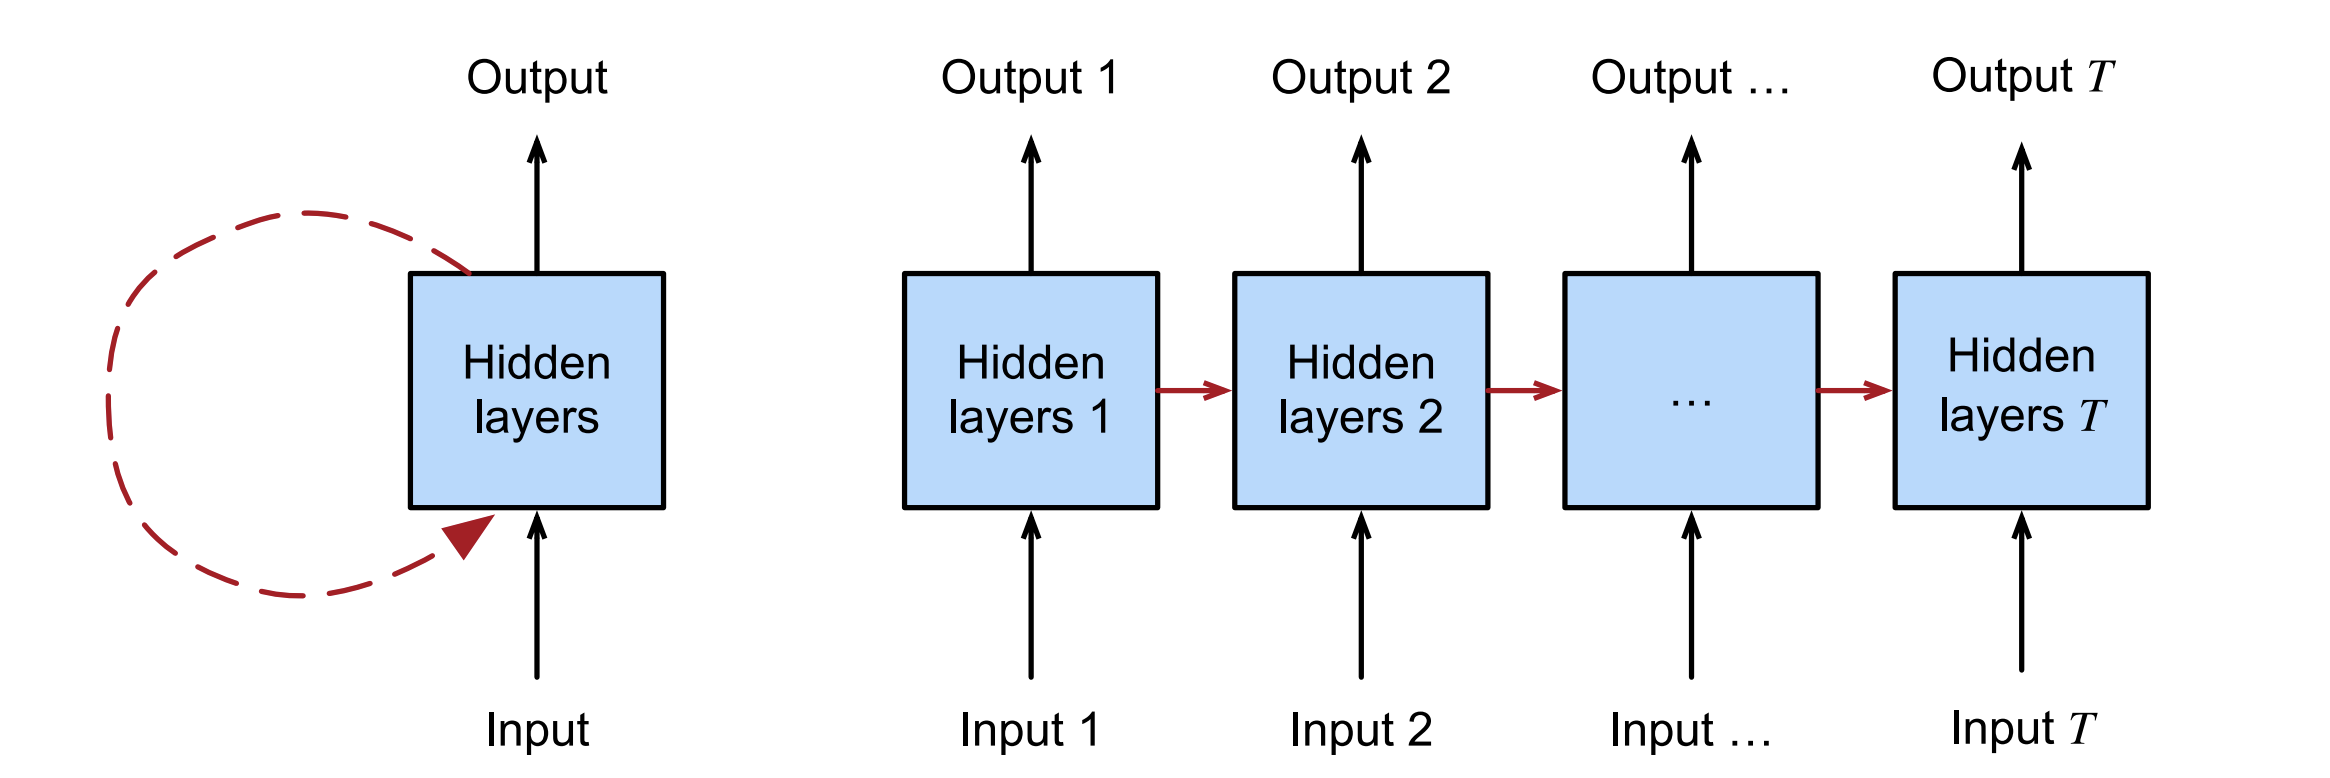
\includegraphics[width=0.7\textwidth]{rnn.png}
        \caption{\centering Diagram of an RNN at a single timestep $t$ (left) and unrolled in time between timesteps $t=1$ and $t=T$ (right) \citep{zhang-2021}.}
        \label{fig: rnn-diagram}
    \end{figure}

    To capture more information from the input sequences, RNNs can consist of multiple internal layers (Figure \ref{fig: deep-rnn}), allowing them to learn higher-dimensional internal representations \citep{bengio-2009}. In this case, each layer $i$ retains its own internal state $h^{(i)}_t$, which is passed on to both the next layer---to compute its state $h^{(i+1)}_t$ at the same input timestep---and reccurred back into itself at the subsequent timestep to compute the state $h^{(i)}_{t+1}$ \citep{zhang-2021}. 

    \begin{figure}[ht]
        \centering
        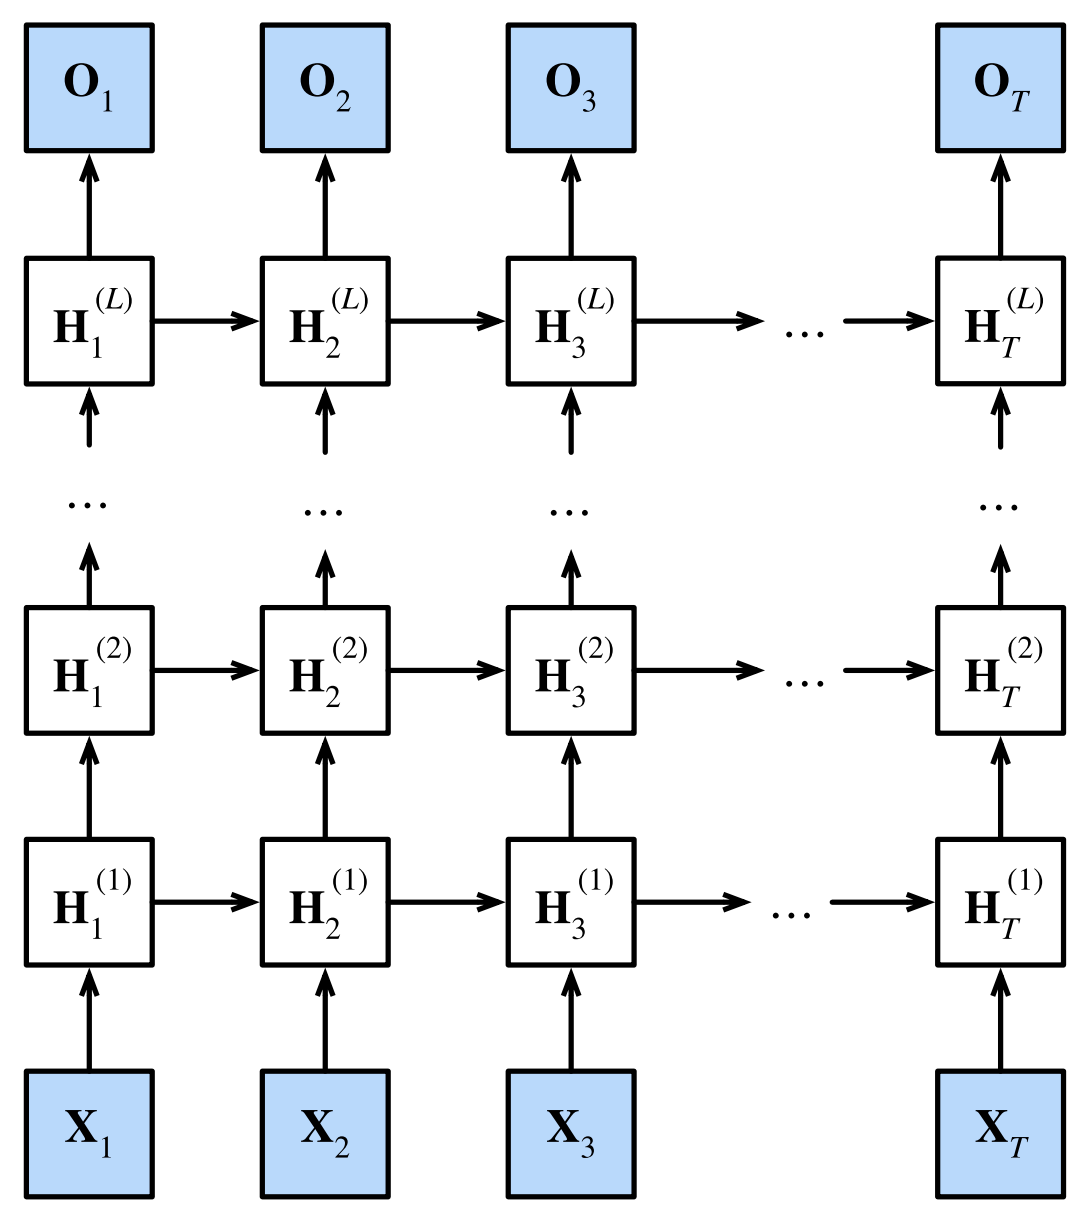
\includegraphics[width=0.25\textwidth]{deep-rnn.png}
        \caption{\centering Diagram of a multi-layer RNN (showing layers $1$ to $L$) with each layer unrolled in time between timesteps $1$ and $T$ \citep{zhang-2021}.}
        \label{fig: deep-rnn}
    \end{figure}


    RNNs are trained through a similar backpropagation process to that used by traditional DNNs. This is done by computing the final output of the network (given an input sequence) and evaluating the loss function between this and the true label to compute the network's error, which is then propagated backwards through both the network's layers and through time to the network's state at each previous timestep \citep{zhang-2021}. This allows the training algorithm to adjust both the network parameters (weights $W$ and biases $b$) and the parameters $\theta^{(g)}$ of the state function $g$.


    \subsection{Applications}

    Recurrent networks have been employed by most recent research into sequence learning. \citet{lipton-2015} explain how NLP tasks and time-series forecasting are the most common avenues explored by researchers utilising RNNs. These two areas have been extensively surveyed in literature; for example, \citet{hewamalage-2021} survey current and future applications of RNNs for time series forecasting, highlighting the recent success of this model architecture at forecasting competitions, such as an RNN-based model by \citet{smyl-2020} winning the \emph{M4 Competition} (in 2019) with an accuracy nearly $10\%$ greater than the utilised baseline \citep{makridakis-2020}.


    \section{Long Short-Term Memory}

    RNNs have been shown to accurately model short-term dependencies within an input sequence. In many cases, however, to understand the full context of a sequence long-term dependencies need to be taken into account. Unfortunately, \citet{hochreiter-1991} and \citet{bengio-1994} have shown that RNNs cannot accurately capture or exploit these long-term dependencies, as contextually relevant elements observed many timesteps ago can be forgotten prematurely. This issue is known as the \emph{short-term memory problem} of RNNs. Whilst several solutions to this problem have been proposed---such as \emph{skip connections} and \emph{leaky recurrent units}---the most widespread approach is the use of \emph{Long Short-Term Memory} (LSTM), presented by \citet{hochreiter-1997}.


    \subsection{Long Short-Term Memory Networks}

    An LSTM is an RNN that uses multiple internal states and parameter matrices to model both short-term and long-term dependencies within sequences. Similarly to an RNN, this architecture contains a core network of one or more layers (each of which is an \emph{LSTM cell}) and information is passed both between these cells (from the input to the output layer) and between timesteps (reccuring the output at time $t-1$ to be input at time $t$). However, instead of a single recurrent state $h_t$, the LSTM contains two: a short-term memory state $h_t$ and long-term memory state $c_t$ used to retain information from far back in the input sequence.

    \begin{figure}[ht]
        \centering
        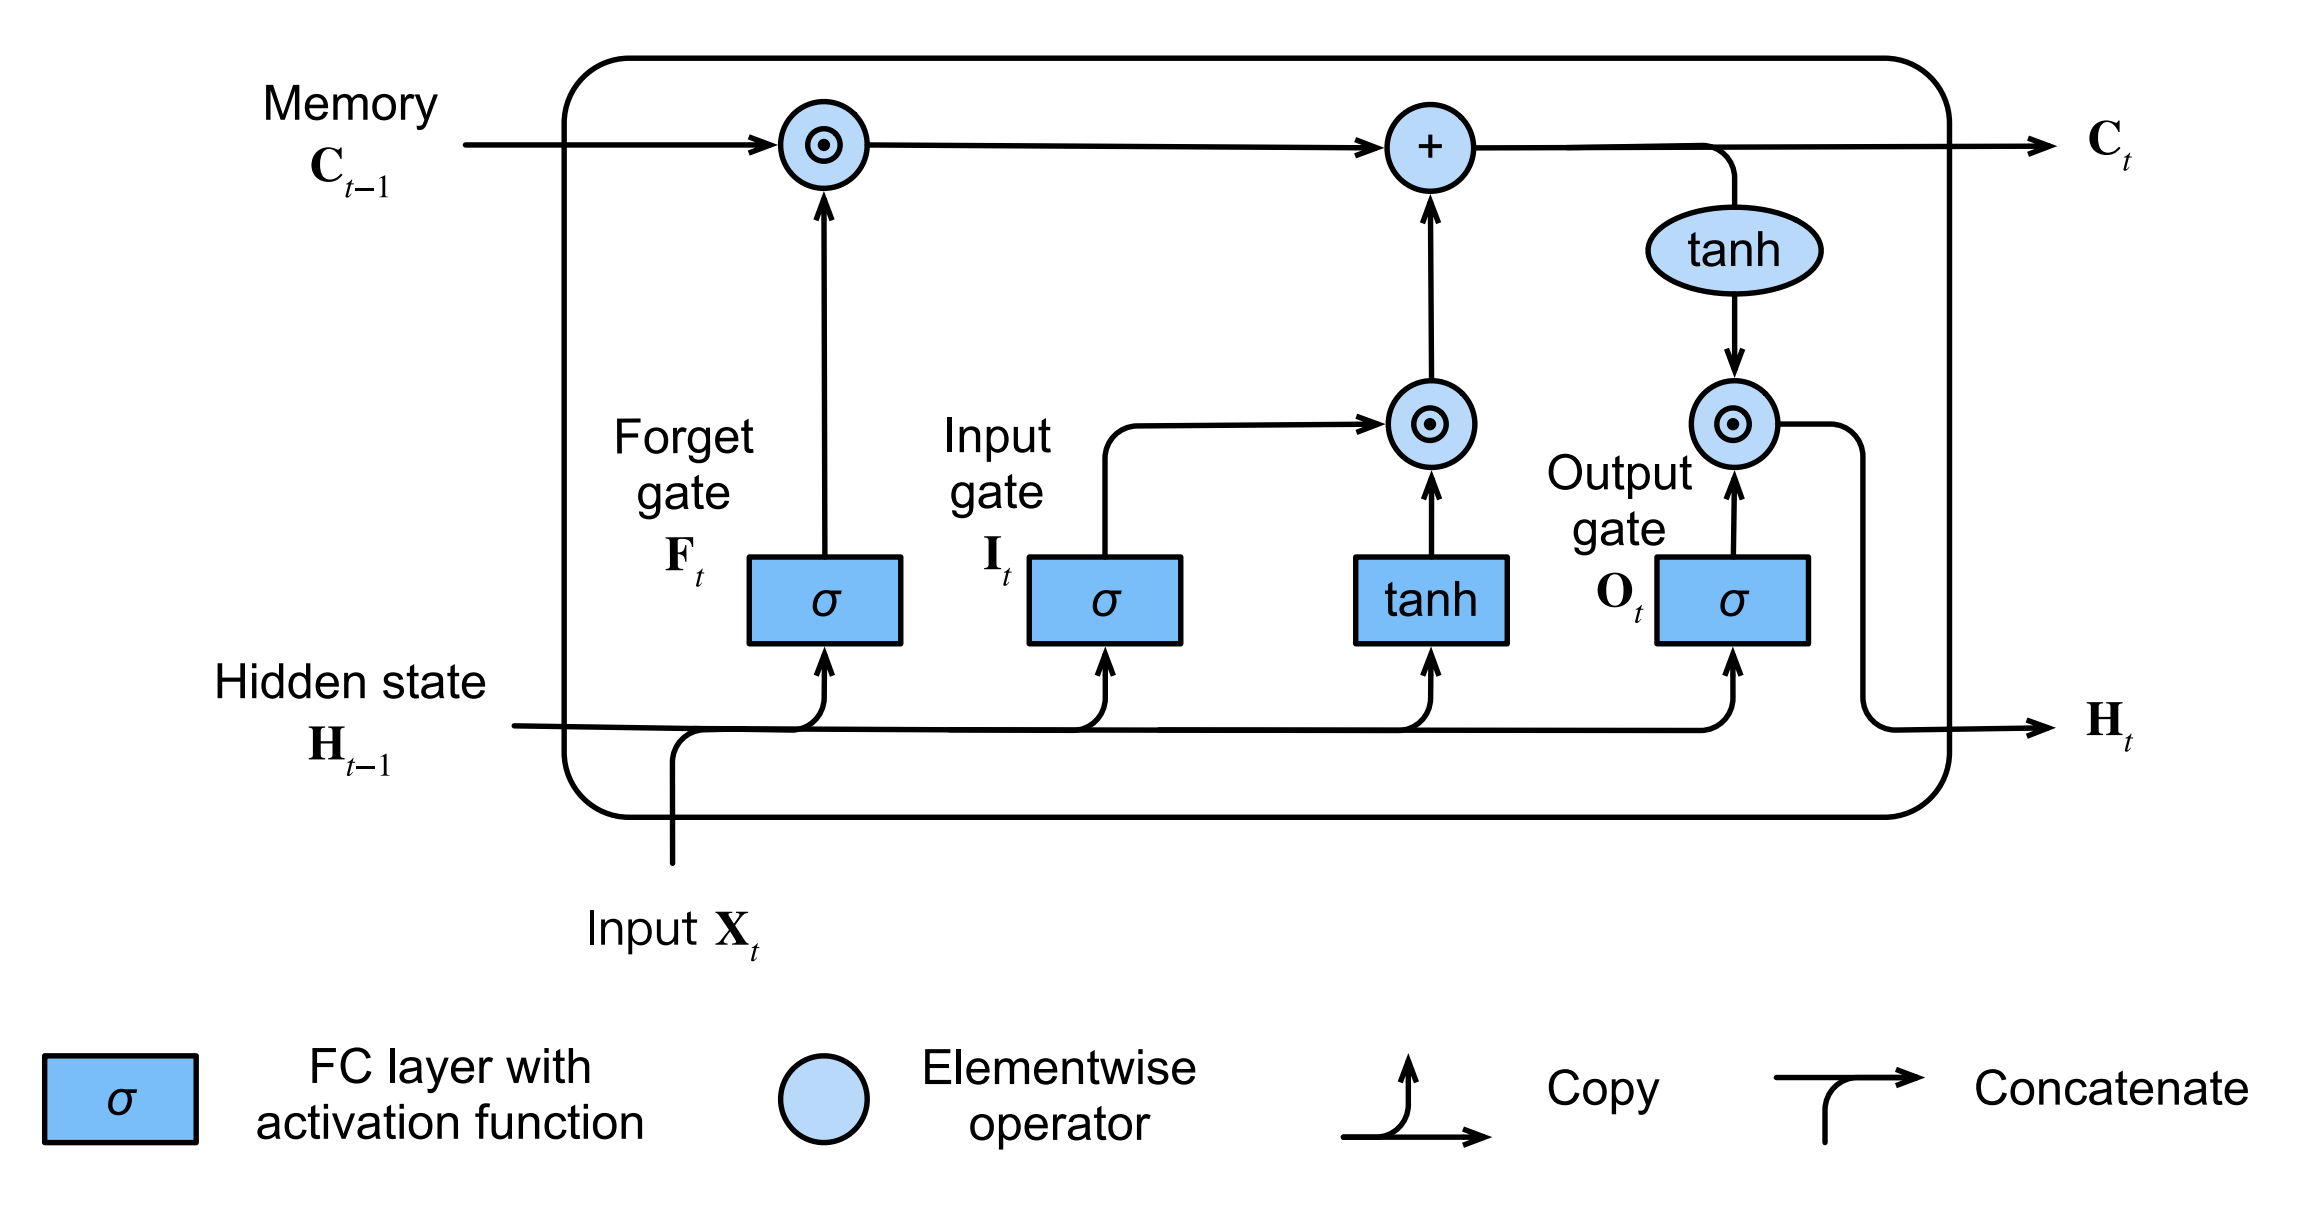
\includegraphics[width=0.5\textwidth]{lstm.png}
        \caption{\centering Diagram of a the logical gates within an LSTM cell \citep{zhang-2021}.}
        \label{fig: lstm}
    \end{figure}

    At each timestep, the preceding long-term state $c_{t-1}$ is input into the LSTM cell (alongside the current sequence element $x_t$) to compute the new states $h_t$ and $c_t$. These updates are achieved through several logical \emph{gates} within the network (Figure \ref{fig: lstm}), each of which is implemented as a single fully-connected ANN layer. Firstly, the \emph{forget gate} is used to decide what information to discard from the previous state $c_{t-1}$. This is computed by multiplying the previous short-term state $h_{t-1}$ and input element $x_t$ with the forget gate's weight matrices $W^{\,(F)}$ and $U^{\,(F)}$ and adding the bias $b^{\,(F)}$, the result of which is passed through the \emph{sigmoid} activation function to produce the intermediate state value $\tilde{c}^{\,(F)}_t$, shown in Equation \ref{eq: forget-gate} \citep{zhang-2021}.

    \begin{equation}
        \label{eq: forget-gate}
        \tilde{c}^{\,(F)}_t = \sigma \Big( W^{\,(F)} \cdot h_{t-1} + U^{\,(F)} \cdot x_t + b^{\,(F)} \Big)
    \end{equation}

    Secondly, when new relevant information is seen in the input sequence, the \emph{input gate} is used to add it to the long-term memory $c_t$. This process similarly uses the short-term state $h_{t-1}$ and current input $x_t$, but evaluates both a sigmoid and \emph{hyperbolic tangent} activation function in parallel on these inputs to decide both which parts of $c_{t-1}$ must be updated and by how much. The result of these two operations are multiplied together to give the second intermediate state value $\tilde{c}^{\,(I)}_t$, shown in Equation \ref{eq: input-gate} \citep{zhang-2021}. Both of these intermediate state values $\tilde{c}^{\,(F)}_t$ and $\tilde{c}^{\,(I)}_t$ are then combined to give the updated long-term state $c_t$ (Equation \ref{eq: long-state}).

    \begin{align}
        \label{eq: input-gate}
        \Big( \tilde{c}^{\,(I)}_t \Big)_{\sigma} &= \sigma \Big( W^{\,(I,0)} \cdot h_{t-1} + U^{\,(I,0)} \cdot x_t + b^{\,(I,0)} \Big) \\
        \Big( \tilde{c}^{\,(I)}_t \Big)_{\tanh} &= \tanh{\Big( W^{\,(I,1)} \cdot h_{t-1} + U^{\,(I,1)} \cdot x_t + b^{\,(I,1)} \Big)} \\
        \tilde{c}^{\,(I)}_t &= \Big( \tilde{c}^{\,(I)}_t \Big)_{\sigma} \cdot \Big( \tilde{c}^{\,(I)}_t \Big)_{\tanh}
    \end{align}

    \begin{equation}
        \label{eq: long-state}
        c_t = \tilde{c}^{\,(F)}_t \cdot c_{t-1} + \tilde{c}^{\,(I)}_t
    \end{equation}

    The third and final gate is the \emph{output gate}, which computes the short-term state $h_t$. The output gate uses the newly computed long-term state $c_t$, input $x_t$, and previous short-term state $h_{t-1}$. A biased weighted sum of $h^{t-1}$ and $x_t$ is computed and fed into the sigmoid function, which is then multiplied by the hyperbolic tangent function evaluated on $c_t$ (Equation \ref{eq: output-gate}). Similarly to within the input gate, the sigmoid evaluation determines the values of $h_{t-1}$ to be updated, and the tangent evaluation determines by how much \citep{zhang-2021}.

    \begin{equation}
        \label{eq: output-gate}
        h_t = \sigma \Big( W^{\,(O)} \cdot h_{t-1} + U^{\,(O)} \cdot x_t + b^{\,(O)} \Big) \cdot \tanh{( c_t )}
    \end{equation}

    This system of gates occurs in every LSTM cell, passing state information from the input to output layer of the network at every timesteps. When the network reaches the final timestep, the short-term state is output as the final network output $y$; note, if the sequence learning problem involves outputting a generated sequence of length $N$ (e.g. forecasting multiple future values), this is produced one element at a time over $N$ additional timesteps that take no input and output the value $y_i = h_{T+i}$.


    \subsection{Applications}

    Both \citet{lipton-2015} and \citet{yu-2019} assert that most state-of-the-art applications within the field of sequence learning use LSTM networks, largely due to their ability to model both long and short-term dependencies, facilitating more accurate predictions; hence, LSTMs have been widely used in both NLP and time series forecasting. For example, \citet{shi-2022} compared the performance of several network architectures for predicting Bejing air quality over time, concluding that LSTMs generated more accurate predictions than simpler RNNs, and demonstrated their improved long-term memory by showing LSTMs outperform other networks even when the context window available to the model is small. This architecture has also been shown to premit the accurate forecasting of financial markets, with research highlighting its ability to accurately capture the complex dependencies within highly variable financial variables \citep{li-2017}; this has facilitated models with impressive performance across financial applications, such as forecasting stock market indices like the S\&P 500 \citep{fjellstrom-2022}, currency pairs on the Foreign Exchange \citep{qi-2021}, and the fluctuations of financial market risk \citep{du-2019}.


    \subsection{The Efficiency of Recurrent Networks}

    Unfortunately, these performance gains inflict a significant computational cost, as research into recurrent architectures has shown that the sequential processing methods vital to their performance also make these models highly inefficient. This tradeoff between accuracy and efficiency has inspired research addressing the energy consumption of these architectures. In their study of compression techniques for LSTMs, \citet{wang-2018} identify the efficiency of such architectures as a core limiting factor restricting their use in resource-constrained domains. This is similarly identified by \citet{zarzycki-2021} in their modelling of chemical reactors; they found that whilst the number of parameters utilised by an LSTM was directly proportional to its modelling performance, higher complexity models inflicted a significant computational cost. 

    Numerous sources, such as \citet{cao-2017} and \citet{feliz-2021}, have deduced that this inefficiency is directly caused by the sequential nature of RNNs. They assert that the many dependencies within LSTM cells (between cells and to the input sequence) restrict how these models can be trained and used. Specifically, cells in an LSTM network take input from both the input sequence and preceding cells; each cell at every network layer and timestep receives both an input vector and two memory states, introducing both temporal dependencies (between cell states at each timestep) and layerwise dependencies (between the output and input of each network layer). Both \citet{cao-2017} and \citet{feliz-2021} identify that this means LSTMs cannot effectively exploit parallelisation, as variables with sequential dependencies must be computed serially. Thus, these networks cannot fully take advantage of the computational speedups provided by specialised hardware such as \emph{Graphics Processing Units} (GPUs) and \emph{Tensor Processing Units} (TPUs) that have been effectively used to parallelise other DL algorithms, making training long and energy-intensive.


    \section{Financial Volatility Modelling}

    Predicting stock price movements is a common example of sequence-to-sequence modelling that has received great attention within the field of DL for finance, with numerous reviews extensively exploring the area (such as \citet{sezer-2019} and \citet{jiang-2021}) and innovative approaches pushing the boundaries of prediction accuracy \citep{darapaneni-2022}. Despite this plethora of research, it is still a challenging task to accurately model price movements in real financial markets due to the complexity of financial systems, non-linear relationships between financial variables, and high-frequency variations in values \citep{timmermann-2004}.


    \subsection{Financial Risk \& Volatility}

    The challenges associated with market price prediction mean that within the finance industry a more helpful use case of sequence-to-sequence modelling is forecasting financial risk. In their white paper explaining the applications and benefits of ML for financial modelling, \citet{laplante-2019} exemplify this sentiment, asserting that ANNs provide the most utility for modelling potential risks. In fact, a recent survey of financial professionals by \citet{chartis-2019} found that $70\%$ of respondents use ML tools in the financial risk sector, majoritively for analysing ``market risk for the trading book" ($51\%$ of respondents) and ``market risk for the banking book" ($44\%$). \citet{peng-2021} similarly assert that modelling risk is currently in high demand due to the large fluctuations, uncertainty, and high volatility exhibited in financial markets, making risk an important consideration when making financial decisions. Furthermore, \citet{mashrur-2020} highlight that financial market risk typically exhibits identifiable trends and reoccuring patterns, facilitating accurate modelling based upon historical data.

    Hence, modelling financial market risk is a popular application of DL; commonly this involves forecasting the \emph{volatility} of an asset or market \citep{peng-2021}. \citet{cavalcante-2016} define volatility as the scale of fluctuations in the pricing of an asset within a financial market over time and is intrinsically related to the risk associated with that asset. \citeauthor{cavalcante-2016} assert that volatility is a vital measure to financial analysis, as it is a key indicator of the state of many economic and external factors that affect financial markets; for instance, in times of economic crisis or political instability, volatility tends to rise, meaning large price variations of assets are likely, and the market is high risk \citep{sezer-2019}. Because of this relationship between volatility and risk, \citet{tino-2001} highlight that volatility changes are typically used as buy and sell signals to investors; \citet{ge-2022} similarly assert market volatility dictates many decisions of market players. Hence, forecasting market volatility is a popular modelling domain.

    \subsection{Measures of Volatility}

    The review of \citet{ge-2022} and volatility model implementation of \citet{tino-2001} both provide comprehensive overviews of the most commonly used measures quantifying volatility: \emph{historical volatility}, \emph{realised volatility}, and \emph{implied volatility}. Implied volatility (IV) is computed given a specific option price, computing the expected volatility associated with that price. Alternatively, realised volatility (RV) is a measure computed directly from the price movements of a market and hence is the volatility actually realised in the underlying financial market. Historical volatility (HV) is a type of realised volatility, which computes the volatility over a preceding time period based upon market closing prices.

    Due to the differences in what these measures represent, each is computed in a slightly different way. Since IV represents an expectation of volatility, it cannot be computed directly from financial market data; instead, IV is estimated through an option pricing model such as the \emph{Black-Scholes model} \citep{black-1973}. On the contrary, RV is computed directly from market price movements over a time window $\tau \to t$ \citep{ge-2022}. This measure is typically calculated as the variation in logarithmic returns $r_t$ of an asset (Equation \ref{eq: return}) over the specified time period. Typically, this time window covers returns observed in the past, which is the HV of that period. When surveying various volatility measures, \citet{ge-2022} found HV to be the most popular, primarily because it provides an intuitive metric that is simple to compute. The most common method of computing HV is to approximate the volatility $v_t$ over the $N$ values of the interval $\tau \to t$ as the standard deviation of logarithmic returns; this is shown in Equation \ref{eq: hv1}, where $\mu_{\tau, t}$ is the mean return over the time interval \citep{ge-2022}. This method of computing HV is used across a wide range of applications within volatility modelling, such as the ANN of \citet{lahmiri-2017} which forecasts the volatility of exchange rates between currency pairs.

    \begin{equation}
        \label{eq: return}
        r_t = \log \Bigg( \frac{c_t}{c_{t-1}} \Bigg)
    \end{equation}

    \begin{equation}
        \label{eq: hv1}
        v_t = \sqrt{ \frac{1}{N} \sum_{t' = \tau}^{t} \big( r_{t'} - \mu_{\tau, t} \big)^2 }
    \end{equation}

    In their review of 35 volatility forecasting ANNs, \citet{ge-2022} found HV was the most popular metric, constituting $71\%$ of research papers; this was followed by other RV measures ($17\%$), and finally IV ($9\%$). Additionally, \citet{ge-2022} explored the most common domains for forecasting volatility, finding the S\&P 500 market to be the most popular (accounting for 12 out of the 35 research papers), primarily due to its accessibility. However, a vast spectrum of models have been developed outside of these domains; for instance, \citet{ge-2022} also explored the use of IV, RV, and HV within the context of stocks, bonds, and other financial indices. Hence, the selection of a volatility measure is typically a domain-specific choice, based upon the different benefits and drawbacks associated with each metric. For instance, due to its reliance upon an options pricing model IV requires options data, and hence cannot be used in other domains. There are also challenges associated with RV and HV; whilst RV has been shown to tend towards an estimate indistinguishable from the latent volatility \citep{andersen-2001}, this accuracy requires data with a high sampling frequency. Additionally, several issues unanimously encompass all volatility estimates, including price irregularities at the tail-ends of return distributions \citep{ozbayoglu-2020} and the complex dependencies between financial variables \citep{timmermann-2004}.


    \subsection{Forecasting Financial Volatility}

    Due to the utility of modelling risk, forecasting market volatility has become a popular domain within both computational finance research \citep{ozbayoglu-2020} and the finance industry \citep{chartis-2019}. Traditionally, financial institutions and researchers have exploited \emph{generalised autoregressive conditional heteroscedasticity} (GARCH) models to forecast volatility. GARCH models have been shown to accurately and reliably capture the characteristics of financial time series \citep{lahmiri-2017}. These models calculate the volatility of a market from a sequence of logarithmic returns $r_0, \dots, r_t$, approximating the volatility $v_t$ at time $t$ as the conditional variance $\sigma_{t}^2$ of returns over the preceding time period. Early work in this field by \citet{akgiray-1989} showed that GARCH models fit training data and forecast volatility more accurately than other models in its class. Similar studies, such as that of \citet{hansen-2005}, have also demonstrated the impressive forecasting accuracy of GARCH models within the foreign exchange market, and shown GARCH's ability to effectively determine clusters of high and low volatility. Largely because of this accuracy, GARCH has become one of the most frequently utilised methods of estimating the volatility of financial time series. Even despite modern methods, this model is still a popular choice, often being used as a baseline to judge the performance of newly proposed volatility forecasting models; for example, \citet{rodikov-2022} used GARCH to contextualise the results of their DNN-based system.


    \subsection{Deep Learning for Volatility Forecasting}

    Whilst traditional forecasting methods have been shown to produce accurate estimations of financial market risk, a significant amount of recent work has applied DL to this domain; for example, \citet{chartis-2019} found that $70\%$ of financial institutions use ML for ``market risk" forecasting. Through analysing the publication rate of research papers in 2018, \citet{sezer-2019} found that volatility forecasting was in the top five uses of DL within financial research. Additionally, in their review of volatility models, \citet{ge-2022} asserted that almost all recent work on forecasting financial volatility relied on ML, largely due to it facilitating higher accuracy modelling of complex time series. DNNs are used to forecast volatility through sequence-to-sequence modelling; a time series of logarithmic returns $r_0, \dots, r_t$ and of previously calculated volatilities $v_0, \dots, v_t$ are used to predict the following volatility sequence $v_{t+1}, \ldots v_{t+n}$ starting at timestep $t+1$ and continuing to forecast a specified number of steps into the future. Namely, the volatility model $M_{\theta}$ is developed that computes the output sequence $y = v_{t+1}, \dots, v_{t+n}$ by approximating the mapping $y = f( r_0, \dots, r_t, v_0, \dots, v_t \lvert \theta )$ between past and future time series.
    
    The performance improvement provided by DL has been exemplified through several studies; for example, \citet{zhang-2022} demonstrated the superiority of DNNs at handling complex interactions and dependencies between financial variables, as their high-dimensional parameter sets allow them to act as better function approximators. Through an evaluation of volatility forecasting models over 23 different stocks, \citet{rahimikia-2020} found that DL gives stronger forecasting power than autoregressive methods like GARCH. \citet{rodikov-2022} drew a similar conclusion, finding that LSTMs could generate a higher test accuracy than other popular models. They also found that RNN architectures were effective at estimating financial market variables like volatility as they do not need to know the parameters of the underlying distribution of the variable being forecast. This is different from models such as GARCH, which uses \emph{maximum likelihood estimation} to approximate the parameters of the return and variance functions of the market.

    Whilst some researchers opt for alternative architectures (such as the CNN-based model of \citet{chen-2018}), the improved accuracy offered by RNNs and LSTMs have established them as a core focus of DL models for volatility forecasting. In their survey of 35 research papers, \citet{ge-2022} found that 9 out of the 21 pure models utilised an RNN, as these networks are a natural fit for time series data. This research typically explores the use of RNNs for forecasting realised volatility within the S\&P 500 market, as \citet{bucci-2020} showed that RNNs outperform all other traditional methods in this domain. Their experimentation demonstrated the ability of an LSTM to capture long-term dependencies within the financial time series, which enabled this architecture to produce accurate forecasts during highly volatile periods.

    Hence, it is clear that the use of DL (in particular RNNs and LSTMs) is an expanding field within financial volatility forecasting, primarily due to the increased prediction accuracy facilitated by these models and algorithms.


    \section{Green AI}

    Whilst complex DNNs are seeing increased adoption across financial modelling, many of these implementations ignore the efficiency concerns associated with DL, such as the memory and energy inefficiency of recurrent networks. The ignorant use of these resource-hungry Red AI models inflicts large ESG costs, as their extreme computational load generates thousands of pounds of carbon emissions over training \citep{strubell-2019}, and limits who can research and employ within high-performance ML systems \citep{bender-2021}. These impacts have spurred recent attention around Green AI, where energy and data-efficient algorithms are developed in an attempt to reduce resource requirements, mitigate environmental costs, and promote inclusivity \citep{schwartz-2019}.


    \subsection{Quantifying the Energy Efficiency of Deep Learning}

    As a simple initial approach to mitigating the ESG cost of DL, many proponents of Green AI suggest that new research papers presenting cutting-edge DNNs should report their training time and resource requirements. In their analysis of 60 DL research papers, \citet{schwartz-2019} found that $90\%$ of papers in the ACL Anthology, $80\%$ of those in the NeurIPS conference, and $75\%$ in the CVPR conference cited accuracy improvements as the main contribution of their work, with only $10\%$ of ACL papers and $20\%$ of CVPR papers contributing a new efficiency result. \citet{schwartz-2019} argue that this demonstrates the lack of reporting surrounding the energy and data efficiency of DL algorithms, highlighting that describing performance contextually with respect to training budgets improves both the sustainability and inclusivity of this work by allowing future work to be compared despite fewer training resources.

    However, a ubiquitous hardware-independent measure of the computational cost of DL algorithms has yet to be agreed upon. \citet{schwartz-2019} describe how the expense $Cost(R)$ of processing the result $R$ using a DNN is proportional to the cost of processing a single instance $I$, the size of the training dataset $D$, and the number of hyperparameters $H$ to be optimised (Equation \ref{eq: cost-r}). They survey several cost metrics, including runtime, parameter count, electricity usage, and carbon emissions; however, they highlight that each of these poses its own challenges, such as the hardware-dependent nature of electricity usage and difficulty in directly measuring carbon emissions. \citet{schwartz-2019} conclude that reporting the total number of \emph{floating-point operations} (FLOPs) to generate the result is the most reliable way to quantify the computational cost, and hence energy efficiency, of an algorithm.

    \begin{equation}
        \label{eq: cost-r}
        Cost(R) = I \cdot D \cdot H
    \end{equation}

    \citet{schwartz-2019} use the competing models \emph{ResNet} (he-2015) and \emph{ResNeXt} (xie-2017) to exemplify how reporting FLOPs can contextualise performance advancements with model efficiency: whilst ResNeXt exhibited a $0.5\%$ accuracy improvement over its predecessor (over the \emph{ImageNet} dataset), it required $35\%$ more FLOPs. \citet{amodei-2018} echo these benefits; however, they highlight that computing the FLOP count of a program is not always trivial. Instead, they assert that the computational cost $Cost(T)$ of a training algorithm $T$ in \emph{petaFLOP/s-days} (pfs-days) is given by the product of the number of GPUs used ($N_{gpu}$), the processing power per GPU in FLOP/s ($P_{GPU}$), the training time ($T_{days}$), and the estimated average utilisation of these GPUs ($U$), typically taken as $33\%$ (Equation \ref{eq: cost-t}). To exemplify this approximation, \citeauthor{amodei-2018} calculated that whilst 2012's leading image classifier AlexNet \citep{krizhevsky-2012} had an approximate computational cost of $0.0058$pfs-days, five years later the innovative DNN \emph{Xception} \citep{chollet-2017} had a cost of $5.0$pfs-days (an increase by a factor of $862$).

    \begin{equation}
        \label{eq: cost-t}
        Cost(T) = N_{gpu} \cdot P_{gpu} \cdot T_{days} \cdot U
    \end{equation}

    Alternatively, further work has attempted to directly quantify the carbon emissions generated by DL algorithms. For instance, \citet{lacoste-2019} proposed the \emph{Machine Learning Emissions Calculator} that computes the $CO_2$-equivalents of an ML algorithm, measuring the environmental detriment caused by energy-intensive Red AI, allowing a direct insight into its environmental cost. However, this approach has yet to receive significant attention.

    This work demonstrates that quantifying the computational, energy, and carbon cost of DNNs is an expanding field within DL research, solidifying quantification methods as a vital first step to raising awareness about the ESG impacts of DL algorithms.


    \subsection{Efficient Neural Network Architectures}

    Once the ESG impact of DNNs has been quantified, new Green AI systems can be developed that minimise their computational cost. As \citet{schwartz-2019} identify, the cost associated with generating a result from a DNN is proportional to that of processing a single instance $I$. Hence, much research into Green AI has focussed on how the architecture of DNNs can be redesigned to minimise computational complexity and the energy expended to process data instances. 


    \subsubsection{Quantisation}
    \label{section: quantisation}

    The record-setting performance of complex DNNs establishes these models are alluring tools for industry players looking to upgrade their workflows; however, in many cases, the upper echelons of performance are neither necessary nor beneficial. For example, \citet{kumar-2020} highlight that in resource-constrained applications (e.g. mobile computing), state-of-the-art DNNs are not feasible as they would quickly engulf the limited power and memory resources. Therefore, researchers have begun to explore how accuracy-efficiency tradeoffs can be made that produce significant decreases in the energetic cost of DNNs whilst minimising the resultant accuracy drop.
    
    Much of this research---explored in the surveys of \citet{xu-2021} and \citet{cai-2022}---has focussed on decreasing computation and memory costs by using lower precision representations of variables and parameters. Typically this is implemented through \emph{quantisation}, where the value of each variable is mapped to discrete quantisation levels that require fewer bits to store. In practice, \emph{deterministic quantisation} is commonly used, with approaches ranging from \emph{uniform quantisation}, where floating-point numbers are mapped to their closest low-bit fixed-point representations, to \emph{clustering quantisation}, where parameters are clustered by value and replaced by the mean of their cluster \citep{xu-2021}. \citet{kumar-2020} demonstrate the performance of uniform quantisation by comparing the DNNs of \citet{courbariaux-2015} and \citet{judd-2016}: \emph{BinaryConnect} \citep{courbariaux-2015} implements an extreme quantisation approach, using only single-bit representations, but inflicts an accuracy drop of $19\%$, whereas, \emph{Stripes} \citep{judd-2016} reduce variable representations from $32$ to $8$-bits whilst inflicting an accuracy drop of only $1\%$. Hence, quantisation is an incredibly adaptable technique and can be contextually used to decrease the computational cost of DNNs.

    \subsubsection{Quantisation-Aware Training}
    \label{section: quantisation-training}

    These methods implement post-training quantisation, which improves the efficiency of models after they have been developed. Further research has explored quantisation-aware training, which aims to reduce the performance drop inflicted by quantisation by utilising it throughout training. For example, \citet{fan-2020b} quantised parameters during training to produce a model that achieved an ImageNet top-1 accuracy score of $80.0\%$ (equivalent to 2017's highest accuracy model ResNeXt) using only $3.3$MB of memory (only $3\%$ of the memory required by ResNeXt). Furthermore, \citet{cai-2022} assert that this training process can be adapted even further to conduct \emph{low-bit training}, where parameters, activation values, and error gradients are all quantised. \emph{DoReFa-Net} \citep{zhou-2016} implemented such low-bit representations, using 1-bit parameters, 2-bit activations, and 6-bit gradients to boost training speed whilst generating an accuracy comparable to AlexNet using 32-bit representations. This demonstrates that quantisation and low-bit representations can be effectively used to produce models with significantly lower memory constraints and energy consumption. Research has also been conducted into quantisation for RNNs and LSTMs: \citet{hubara-2016} explored the effectiveness of quantising weights and activations within recurrent networks, whilst \citet{he-2016} proposed quantising LSTM gates. However, whilst investigating quantisation for RNNs, \citet{ott-2017} found that low-bit training was not ubiquitously effective in this context; thus, they concluded \emph{mixed-precision training} should be used for RNNs, where weight matrices are quantised but activation values retain higher precision representations.


    \subsection{Efficient Training Algorithms}
    \label{section: efficient-training}

    Whilst the efficiency of a DNN's architecture is essential to minimising the energy expended on each data instance, it is also important to minimise the length of DNN training. Hence, a significant amount of research within Green AI focuses on energy-efficient training algorithms that attempt to reduce the number of iterations necessary to train an accurate model.


    \subsubsection{Transfer Learning}

    Possibly the most common method of reducing the length of DNN training is using a pre-trained model developed for an analogous task. This method---discussed by \citet{strubell-2019}, \citet{walsh-2021}, and \citet{schwartz-2019}---is known as \emph{transfer learning}, which uses an existing pre-trained \emph{base model}, and tunes its parameters over a new training dataset that covers a new domain. Since the base model has already learned a general ability to complete a similar task, the new target model requires only a short, inexpensive retraining process, where the model is fine-tuned to accurately capture information from the new domain. Both \citet{strubell-2019} and \citet{walsh-2021} identify that transfer learning significantly reduces the resources required to train a DNN and allows their application to fields with limited amounts of data. For example, \citet{wang-2020} used transfer learning to apply ResNet to the \emph{Stanford Dogs 120} dataset, a small collection of only $20,580$ images (only $1.7\%$ of the size of the ImageNet dataset used to train ResNet). The use of transfer learning allowed \citeauthor{wang-2020} to develop a model that had an accuracy $11.07\%$ greater than any other DNN developed for this domain and reduced the required training iterations by a factor of $10$. This demonstrates that transfer learning is a simple but effective method for reducing the training cost of DNNs, which allows models to be developed for niche domains and minimises the energy required to train accurate ML models.


    \subsubsection{Initialisation}

    Instead of directly copying a base model, its parameter values can be used as a starting point to optimise the parameter set of a new DNN. This is known as \emph{initialisation}, which is the process through which the initial values of a parameter set are chosen. Initialisation is incredibly important, as \citet{xu-2021} found that the rate of convergence of a network's parameters towards their optimal values heavily depends upon their initial values. Furthermore, \citet{hanin-2018} found that primitive initialisation methods (such as random initialisation) can lead to slow training, or even result in parameter values never converging.

    Both \citet{hanin-2018} and \citet{xu-2021} evaluate alternative methods for initialising a DNN. \emph{Feature-based initialisation} assigns borrowed parameter values to a subset of the new DNN's parameters and keeps these fixed during training (improving generalisability), whereas \emph{fine-tuning-based initialisation} trains all new and borrowed parameters, providing greater specialisation. Alternatively, \emph{supervised initialisation} pre-trains the new DNN over similar datasets or for analogous tasks, then reuses these representations as a starting point for training over the target task and dataset. For example, \citet{lin-2021} initially pre-trained their language model as a general multilingual translator, before specifically applying the network to translate between language pairs. \emph{Self-supervised initialisation} takes this concept further, allowing pre-training to be conducted without supervised data by learning general representations over an unlabelled dataset \citep{peters-2018}.

    Hence, this established research demonstrates the importance of selecting a suitable initialisation method when developing a new DNN based upon the chosen application and architecture, as the starting point of training can drastically reduce the energy expended to generate an accurate model.


    \subsubsection{Progressive Training}
    \label{section: progressive-training}

    \emph{Progressive training} \citep{xu-2021}, also known as \emph{greedy layer-wise pre-training} \citep{xu-2018}, builds upon this concept of pre-training. This training approach constructs a model layer-by-layer by iteratively adding a new layer and tuning its parameters. This builds the DNN in a bottom-up approach, whereby the network first trains lower layers to accurately represent low-level features of the input, then trains higher layers based upon the learned parameters of the preceding layers. After adding the desired number of layers, all parameters are optimised in a concluding tuning phase. In theory, this reduces the computational cost of training a DNN, as training shallow, single-layer networks is significantly simpler and less resource intensive than training full, deep networks \citep{xu-2021}. Furthermore, \citet{xu-2021} assert that the parameters of later layers are optimised faster, as values are updated based on information already learnt about the features of the input during preceding pre-training rounds. This approach has been successfully used by \citet{yang-2020} who reduced the total training time required by the language model BERT by over $110\%$ (from $85$ to $40$ hours) without degrading accuracy.

    Progressive training can be implemented through either \emph{supervised layer-wise pre-training} or \emph{unsupervised layer-wise pre-training}. Supervised approaches, such as that of \citet{ienco-2019}, train individual layers through supervised learning; for example, if building a forecasting model, each layer is independently trained to predict the future elements of a sequence \citep{xu-2018}. Starting by training a shallow network consisting of only an input layer, one hidden layer, and an output layer, the model iteratively gets deeper; this is achieved by first removing (and saving) the output layer, then fixing the values of all previously trained parameters, adding a new hidden layer, appending the saved output layer, and finally training the parameters of this new layer. Once a network of the desired depth has been constructed, the parameters of all layers are unfixed, and a short training round is conducted over the full network, where the parameters found during pre-training are used as a starting point for deducing the optimal global parameter set. 

    Unsupervised approaches---such as the implementations of \citet{xu-2018} and \citet{sagheer-2019}---train each layer as an \emph{auto-encoder}. Autoencoders are a type of ANN that learns to output an encoded representation of its input; they are trained through unsupervised learning, minimising the difference between the network's input and output vectors \citep{pinaya-2019}. In unsupervised layer-wise pre-training, network layers are also built up iteratively as unsupervised autoencoders, learning to output a representation of the input vector. This unsupervised learning is repeated over the entirity of pre-training, resulting in an autoencoder network of the desired depth \citep{sagheer-2019}. Subsequently, the full network is tuned, repurposing the model to the desired task by discarding the autoencoder output layer used during pre-training, and appending a new output layer for the desired task. With all parameters unfixed, the network then undergoes training, starting from the parameter set found during pre-training, and optimising the entire network's performance in the chosen domain \citep{sagheer-2019}.

    Research into layer-wise pre-training typically centres around improving the efficiency of training recurrent networks, as RNNs have been identified as one of the most sensitive architectures to parameter initialisation. \citet{ienco-2019} showcase how supervised layer-wise pre-training can be used to produce an RNN-based sequence classifier that exceeded the accuracy of comparable models in a number of applications. Both \citet{xu-2018} and \citet{sagheer-2019} demonstrate that unsupervised layer-wise pre-training is effective at improving training efficiency while preserving accuracy. By comparing LSTM models initialised with layer-wise pre-training to a simple randomised initialisation, \citet{xu-2018} exemplified the performance and efficiency benefits of this technique across a number of domains, including image recognition and sequence-to-sequence modelling. \citet{xu-2018} found that unsupervised layer-wise pre-training of LSTMs induced faster convergence toward the optimal parameter set, as their initialised values were located close to local minima of the loss function. They also found that the resultant model exhibited a smaller test error, suggesting this training method improves the generalisability of LSTMs. Similarly, \citet{sagheer-2019} compared unsupervised pre-training and random parameter initialisation, focussing on deep LSTMs for time series forecasting. They discovered that the layer-wise method produced better and faster convergence, especially when forecasting collections of correlated variables; this suggests unsupervised layer-wise pre-training is a good fit for forecasting complex financial time series.

    Hence, progressive training has been shown to decrease the time and energy required to train DNNs and RNNs, and develop networks that capture complex dependencies between variables, indicating that this algorithm will be effective for modelling complex financial time series.


    \subsection{Data Efficiency}

    A common trend in state-of-the-art DL algorithms is a reliance upon vast datasets; \citet{bender-2021} summarise this work as following a philosophy of ``there's no data like more data". For example, the image classification model of \citet{mahajan-2018} produced record-breaking accuracy, but achieved this by training over a dataset of $3.5$ billion images, three orders of magnitude larger than the commonly used \emph{Open Images Dataset} (of $9$ million instances). Both \citet{schwartz-2019} and \citet{bender-2021} assert that these extreme datasets are a major problem with Red AI, highlighting that dataset size is a significant contributor to the computational and energetic cost of a model; thus, Green AI often attempts to minimise these datasets and their associated costs.


    \subsubsection{Inefficient Use of Data}

    Both \citet{bender-2021} and \citet{walsh-2021} highlight that much of this computational cost is due to the inefficient use of data, as models train over vast datasets, most of which are not beneficial to learning. \citeauthor{bender-2021} suggest that more time should be put into carefully curating specialised datasets for each model and domain, minimising the time and energy wasted on unhelpful data instances. \citet{aljarrah-2015} further note that current ML systems are not intelligent enough to efficiently deal with significantly increased data loads. They highlight that commonly used optimisation methods (such as gradient descent) require substantial work to locate global optima; thus, when applied to large datasets, these methods accumulate an extreme computational cost.

    Furthermore, there can often be a conflict between the architecture size and training dataset size, as small ANNs typically require more data to achieve comparable accuracy. \citet{bender-2021} found that the model \emph{ALBERT} \citep{lan-2020}, which attempts to recreate the performance of the complex network BERT using a smaller parameter set, required large amounts of data to force advances in accuracy beyond that typically achieved by compact networks. This demonstrates that when developing efficient DL algorithms, a balance must be drawn between model size and dataset size, as both contribute to their computational cost.


    \subsubsection{Reducing Data Requirements}

    Several avenues have been proposed within Green AI for reducing data requirements whilst preserving accurate performance. \citet{xu-2021} discuss a variety of dataset reduction techniques; these methods typically rely on pre-trained models analygous to those described in Section \ref{section: efficient-training}. Namely, pre-trained models can exploit self-supervised learning to initialise near-optimal parameters without needing labelled data. This reduces data requirements as energy does not need to be expended labelling the data required for pre-training, and the initialised model converges faster downstream during the full training stage \citep{xu-2021}. \emph{Contrastive learning} \citep{chen-2020} is raised by \citet{xu-2021} as a commonly used pre-training method for reducing data requirements in CV. This approach focuses on learning pairwise relationships between data instances, representing similar pairs close together in the data space and pushing divergent pairs far apart, thus allowing the dataset to be constricted. \citet{xu-2021} further highlight the effectiveness of \emph{prompt learning} \citep{liu-2021}, where data instances are labelled with a task-specific template known as a \emph{prompt}, reducing the training dataset size as a single prompt can represent up to $100$ individual data instances. 


    \subsubsection{Active Learning}
    \label{section: active-learning}

    Possibly the most widely explored method for reducing the data requirements of training DNNs is \emph{active learning}. This method, whose utility to DL has been extensively explored by surveys such as that of \citet{ren-2021}, aims to reduce training costs by selecting a subset of data instances from the full data space that are believed to provide the most utility to the model's learning process. 

    Active learning is a training algorithm that significantly diverges from traditional algorithms that iteratively train a network over the full dataset $D$ of $N$ instances. This algorithm splits the training data $D$ into smaller chunks, utilising it as either a \emph{stream} or a \emph{pool}. \emph{Stream-based active learning} individually picks data instances from $D$ and evaluates whether to train over this single instance, feeding useful instances into the DNN \citep{ren-2021}. More commonly, \emph{pool-based active learning} is implemented; at each round of training, this algorithm selects a pool of the $n_{sample}$ most useful instances from the full dataset, and trains the network over these \citep{ren-2021}. Specifically, pool-based approaches divide $D$ into the pool set $P$ and validation set $V$; at the start of training, the pool set $P^{\,(0)}$ is empty, and the validation set $V^{\,(0)}$ contains all elements of the full dataset $D$. To begin training, an initial pool $P^{\,(0)}$ of $n_{sample}$ data instances (known as the \emph{seed}) must be sampled from the full dataset; most simplistically, these are drawn at random. These sampled values are then moved from the initial validation set $V^{\,(0)}$ to the new pool; hence we have the new datasets $P^{\,(1)}$ (where $\big\vert P^{\,(1)} \big\vert = n_{sample}$) and $V^{\,(1)}$ (where $\big\vert V^{\,(1)} \big\vert = N - n_{sample}$). After the seed has been selected, the first round of training can be conducted, where the DNN is trained over pool $P^{\,(1)}$. This partially trained DNN is then used to predict the labels of the remaining $N - n_{sample}$ data points in the validation set; these predictions are fed into an \emph{importance function} scoring each instance in $V^{\,(1)}$ according to its utility to the learning process of the DNN. The $n_{sample}$ instances with the highest importance score are then selected from the validation set and moved into the pool; thus, we have the new datasets $P^{\,(2)}$ and $V^{\,(2)}$ where $\big\vert P^{\,(2)} \big\vert = 2 n_{sample}$ and $\big\vert V^{\,(2)} \big\vert = N - 2 n_{sample}$. This process is repeated over multiple training iterations, evaluating the importance function and expanding the pool set, until either a dataset size, iteration count, or accuracy threshold has been reached \citep{ren-2021}.

    Both \citet{ren-2021} and \citet{xu-2021} assert that active learning drastically increases the data efficiency of training DNNs. \citet{ren-2021} found that this algorithm can theoretically achieve an exponential improvement in the time required to label training data; they also found it could successfully deal with high-dimensional data and train efficient but accurate models for sequential data. \citet{xu-2021} similarly assert that active learning significantly reduces the time and energy wasted on redundant data instances that do not benefit the DNN's learning. Furthermore, \citet{ren-2021} note that the resources required to evaluate the importance function does not undermine the efficiency gains provided by the iterative learning process, as this function can be efficiently implemented to inflict a negligible computational cost. 

    Hence, active learning has been shown to reduce the data requirements of training DNNs. Furthermore, whilst training over time series data introduces further complexity due to the temporal nature of variables, \citet{peng-2017} and \citet{zimmer-2018} have demonstrated the feasibility of active learning in this field, demonstrating that this approach has the potential to improve the data and energy efficiency of high-performance sequential models such as those used within volatility forecasting.


    % --------------------  EXPERIMENTS ----------------------
    \newpage
    \chapter{Methodology}
    \label{chapter: experiments}

    \section{Introduction to Experiments}

    This study investigates how energy and data-efficient Green AI algorithms can be applied to finance. Specifically, this research will explore how DNNs for financial volatility forecasting over the S\&P 500 market can be trained efficiently whilst preserving accuracy, in an attempt to demonstrate how the resource requirements, energy expenditure, and environmental impacts of Fintech can be reduced. Hence, this experimentation highlights the importance of considering the ESG impacts of DL, and demonstrates that high-performance DNNs can be utilised in this domain without sacrificing the SDGs of sustainable finance. Additionally, this study intends to illustrate how efficient training algorithms can be applied outside of the the existing research applications of NLP, CV, and mobile computing, expanding the scope and impact of Green AI.

    To illustrate the utility of Green AI to finance, two core research hypotheses are tested. Firstly, this study explores the question: \emph{can using Green AI algorithms reduce the training time required to develop an accurate volatility forecasting model?} Experimentation into the hypothesis that energy-efficient algorithms can produce accurate volatilty models aims to fill the research gap between the goals of sustainable finance and the expanding use of DL in Fintech by minimising the computational cost of training DNNs. Secondly, this research examines the further question: \emph{can Green AI algorithms reduce the data requirements of training an accurate volatility forecasting model?} This extended study explores the hypothesis that Green AI not only facilitates a direct reduction in training time and energy consumption, but additionally provides a way reducing the data requirements of DL. By minimising data requirements, the cost of training DNNs can further be reduced, as less energy is expended labelling training data and learning over redundant instances that do not benefit performance \citep{schwartz-2019}. Furthermore, the use of smaller datasets improves the inclusivity of this field, as researchers and market players do not need to invest in expansive computer memory or cloud storage to train accurate volatility models \citep{strubell-2019}. Hence, the exploration of both hypotheses contributes to the field in several ways: expanding the applications of Green AI, reducing the environmental cost of Fintech, and improving the inclusivity of finance.

    To investigate these hypotheses, this research is divided into three core studies. Initially, the dataset over which volatilty forecasting is conducted is presented in Section \ref{section: dataset}, and the metrics used to analyse the accuracy and efficiency of the developed DL models and algorithms are outlined in Section \ref{section: metrics}. Following this, model architecture implemented in this research is presented in Section \ref{section: baseline}; a traditional training algorithm is presented through which a baseline model is developed. Following this, Chapter \ref{chapter: energy-extensions} explores the Green AI algorithms implemented that attempt to improve the energy efficiency of training the LSTM network. A comprehensive explanation of these methods and their utility is given, exploring their potential to reducing the computational cost of DNN training. Finally, Chapter \ref{chapter: data-extensions} explores the minimisation of data requirements through Green AI methods; an adapted training algorithm is presented that aims to decrease the training dataset size, hence facilitating further computational cost, energy consumption, and carbon emission reductions.


    \section{Dataset}
    \label{section: dataset}

    To evaluate the use of Green AI in finance, the specific domain of financial market volatility forecasting was chosen, as it is currently one of the most popular applications of DL within finance; in fact, volatility forecasting is within the top five most popular uses of DL within financial research \citep{sezer-2019}. Furthermore, \citet{chartis-2019} demonstrated that this domain is a popular application of DL within the financial industry, finding that $70\%$ of financial institutions use ML for risk analysis, most commonly for forecasting ``market risk". This extensive use is primarily due to the superior accuracy provided by DL: \citet{chartis-2019} found that $44\%$ of financial firms are motivated to use DL by the promise of ``greater accuracy", and DNNs have been shown to outperform traditional volatility forecasting methods \citep{rodikov-2022}. For this reason, it is clear that volatility forecasting is a characteristic example of the use of DL within finance; hence, showing the applicability and benefit of Green AI within this domain acts as an exemplar of how the energy consumption of DL for finance in general can be reduced, and the ESG impacts of Fintech mitigated.

    % \begin{figure}[ht]
    %     \centering
    %     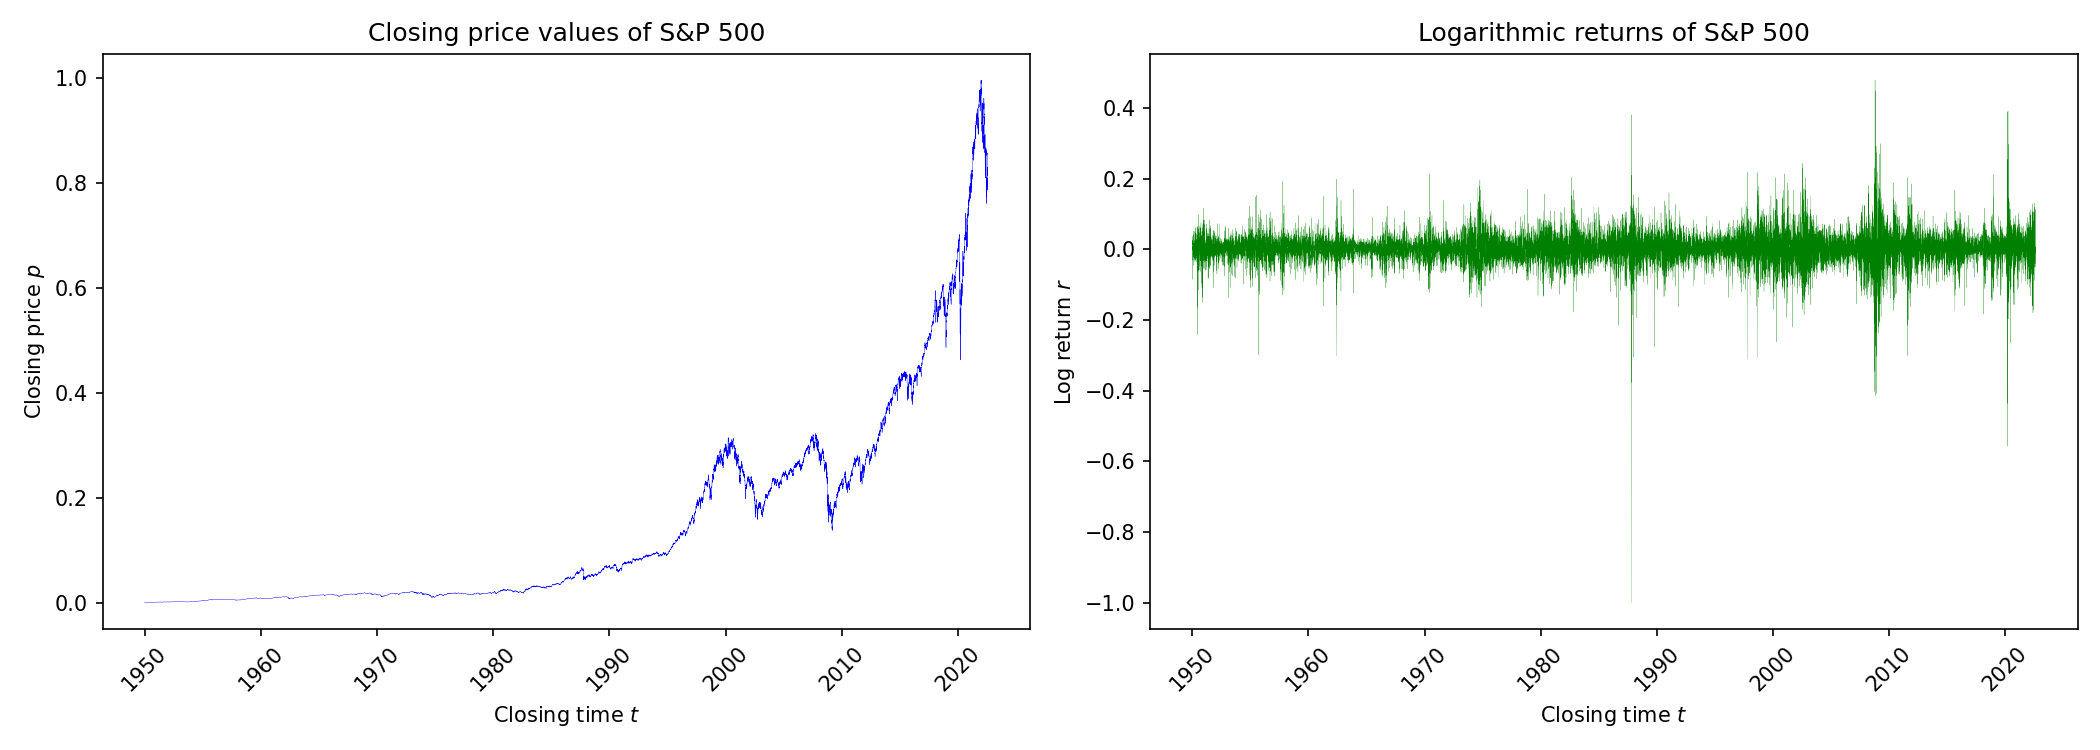
\includegraphics[width=0.5\textwidth]{dataset.png}
    %     \caption{\centering Time series of closing prices of the S\&P 500 market used within the training dataset.}
    %     \label{fig: prices}
    % \end{figure}

    The \emph{Standard \& Poor's 500 Index} (S\&P 500) is a stock market index capturing the price movements of 500 leading US companies. It is often regarded as one of the best indicators of the performance of the global stock market; thus, S\&P 500 data has become a popular target for time series modelling \citep{thakkar-2021}. \citet{ge-2022} found that DNNs were most commonly used for forecasting the volatility of the S\&P 500 market (accounting for 12 of the 35 works surveyed), primarily due to the accessibility of data. Therefore, to ensure universal results charcateristic of this domain, S\&P 500 data was chosen as the specific modelling domain explored within this research.

    \begin{figure}[ht]
        \centering
        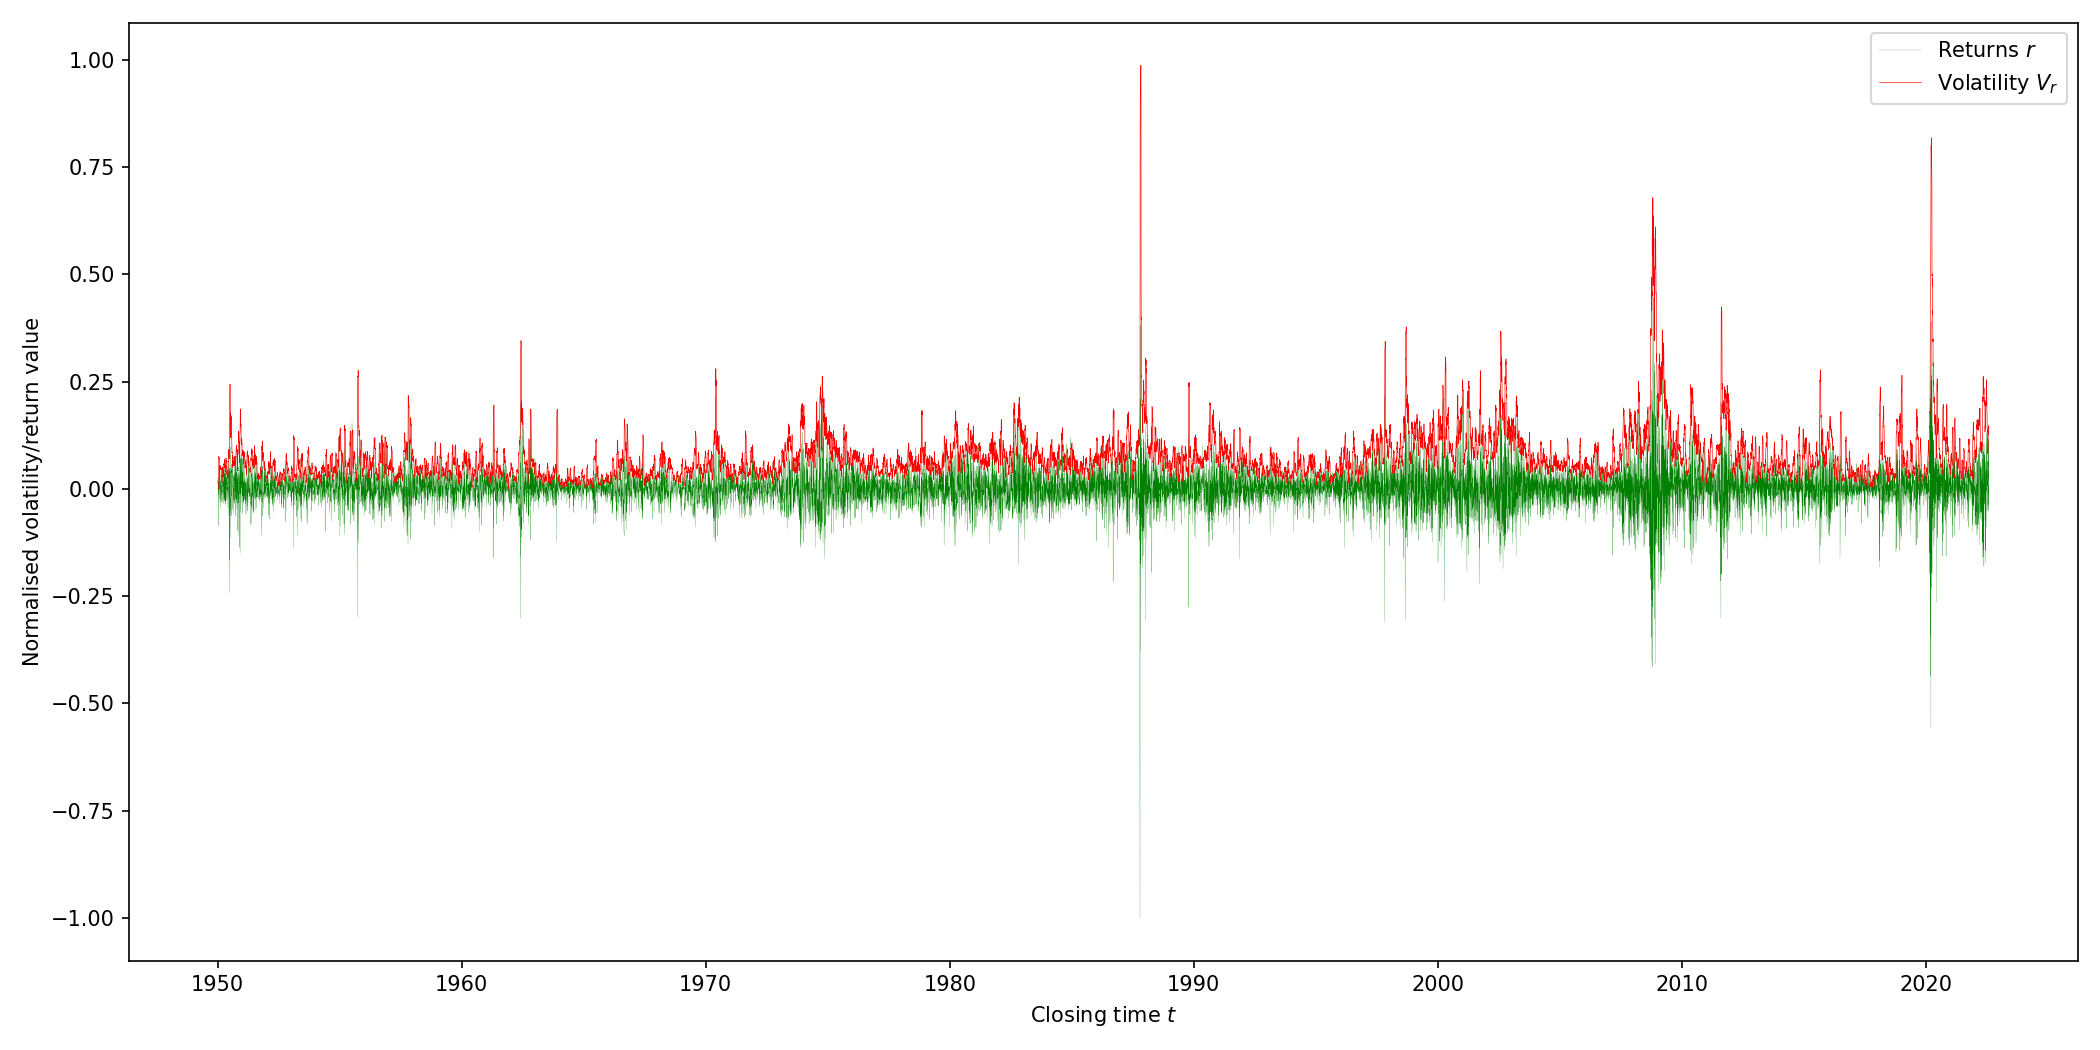
\includegraphics[width=0.7\textwidth]{volatility.png}
        \caption{\centering Time series of daily returns of prices over the S\&P 500 market, overlaid with the computed historical volatility time series for the same period.}
        \label{fig: ret-vol}
    \end{figure}

    To enable sequence learning, the S\&P 500 data is represented as a multivariate time series consisting of $18261$ daily sampled timesteps between the fifth of January 1950 and the first of August 2022. This period and sampling frequency were specifically chosen as daily data strikes an effective compromise between maintaining a reasonable dataset size and having a high enough data frequency to permit detailed analysis \citep{rodikov-2022}. Each timestep maintains the value of seven variables of the S\&P 500 market: the daily \emph{open}, \emph{close}, \emph{high}, and \emph{low} prices, trading \emph{volume}, associated \emph{return}, and market \emph{volatility} (Table \ref{table: time-series}). The return $r_t$ is computed as the logarithmic change in closing price from the previous day (Equation \ref{eq: return}), and used to calculate the HV as the standard deviation $\sigma_{t}^2$ of returns over the past $10$ days; namely, $\sigma_{t}^2$ is computed from the time series $r_{\tau}, \ldots, r_{t}$ over the time interval $\tau \to t$ (where $\tau$ is $9$ timesteps behind the current timestep $t$). The HV is calculated through Equation \ref{eq: hv1}, iteratively constructing the volatility time series $v_0, \ldots, v_t$; this echoes the approach of \citet{lahmiri-2017} who also developed an ANN for volatility forecasting. The time series of returns and volatilites over the full period is showcased in Figure \ref{fig: ret-vol}. Historical volatility was chosen as the metric to be forecast as it was identified by \citet{ge-2022} as the most commonly explored way of measuring market volatility. Furthermore, HV has been utilised in many innovative explorations of this field, such as \citet{rahimikia-2020} and \citet{rodikov-2022} who both demonstrated the exceptional forecasting accuracy of DNNs for this metric.


    % \begin{table}[ht]
    %     \centering
    %     \begin{tabular}{|l|lllllll|} 
    %         \hline
    %         \textbf{Timestep} & \textbf{Open} & \textbf{Close} & \textbf{High} & \textbf{Low} & \textbf{Volume} & \textbf{Return} & \textbf{Volatility}  \\ 
    %         \hline
    %         2022-08-01 & 0.855942 & 0.855188 & 0.856735 & 0.853413 & 0.309027 & -0.025801 & 0.140913    \\ 
    %         \hline
    %         2022-07-29 & 0.850728 & 0.857619 & 0.855739 & 0.849899 & 0.333186 & 0.128754  & 0.145031    \\ 
    %         \hline
    %         2022-07-28 & 0.837990 & 0.845556 & 0.843038 & 0.831855 & 0.338870 & 0.110068  & 0.147466    \\ 
    %         \hline
    %         2022-07-27 & 0.822442 & 0.835378 & 0.834864 & 0.823165 & 0.312798 & 0.235645  & 0.129777    \\ 
    %         \hline
    %         2022-07-26 & 0.822814 & 0.813996 & 0.816945 & 0.814652 & 0.269089 & -0.105961 & 0.126826    \\
    %         \hline
    %     \end{tabular}

    %     \caption{\centering The final 5 timesteps of the multivariate time series (in reverse chronological order).}
    %     \label{table: time-series}
    % \end{table}


    The implemented DNNs use the volatility time series $v_0, \ldots, v_t$ to forecast the daily HV of the S\&P 500 at a single future timestep $t+1$ (outputting the prediction $\hat{v}_{t+1}$). To train and test the model, the full time series is broken down into individual sequences of $10$ timesteps, where each data instance is a 10-step subsequence of the entire time series, enumerating the progression of the seven intrinsic variables. Hence, each data instance in the full dataset is in essence $7$ small time series; one for the closing prices, returns, volatilities, and so on. Each of these variables was normalised through min-max scaling, restricting their values to the range 0--1 (except the returns, which were allowed to fluctuate between $-1$ and $1$ to permit negative values); this scaling approach was similarly used by \citet{rodikov-2022}, who highlighted that normalisation is essential to a stable and efficient training process.

    % (Table \ref{table: time-series})


    \begin{figure}[ht]
        \centering
        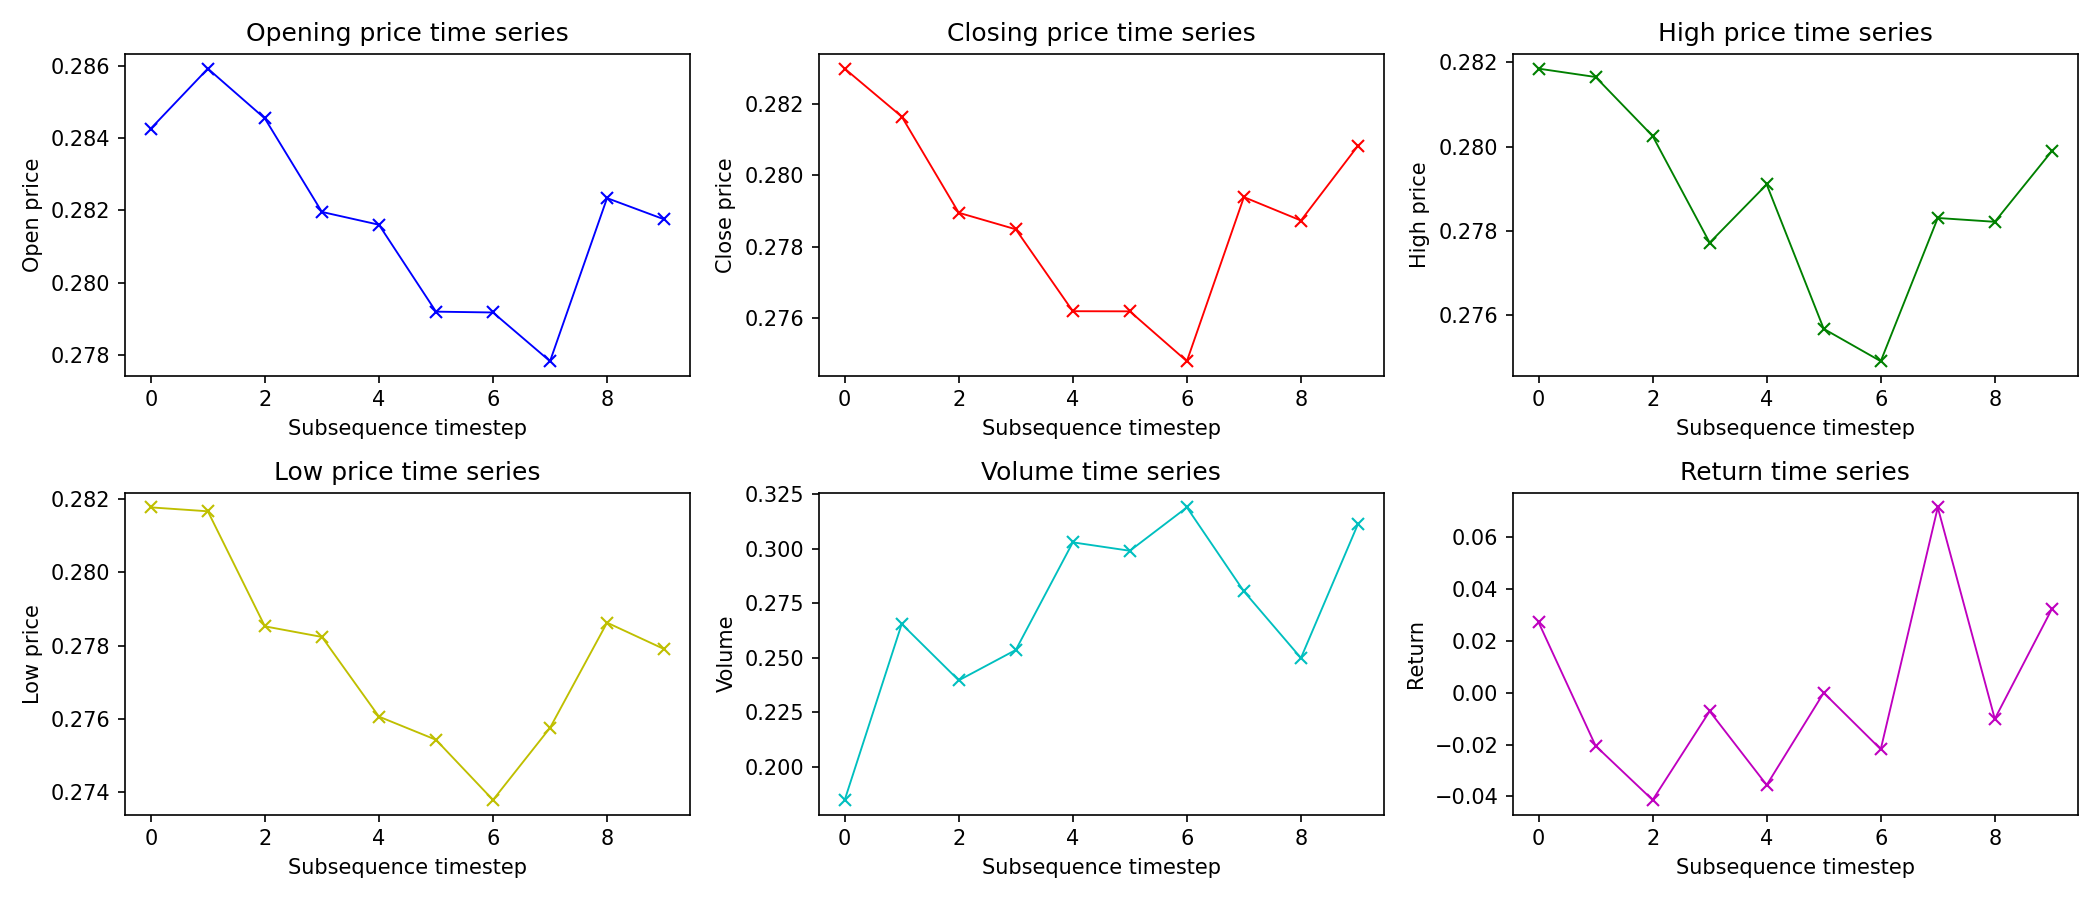
\includegraphics[width=0.8\textwidth]{subsequences.png}
        \caption{\centering Subsequences comprising the multivariate time windowed time series for an example instance from the training dataset.}
        \label{fig: subsequences}
    \end{figure}


    The modelling task was set up as a sequence-to-sequence problem, where each multivariate $10$-step time series is input into the DNN to predict the subsequent value $\hat{y}_t = \hat{v}_{t+1}$. Thus, each pass through the model predicts the volatility of the S\&P 500 market at timestep $t+1$ through analysing the preceding multivariate time series over steps $(t-9) \to t$. This is shown through Figure \ref{fig: subsequences}, which (for a randomly selected data instance) gives an example of subsequences that make up each multivariate $10$-step time series, and Figure \ref{fig: volatility-subsequence} demonstrating a volatility subsequence with the true label $v_{t+1}$ to be predicted by the model.


    \begin{figure}[ht]
        \centering
        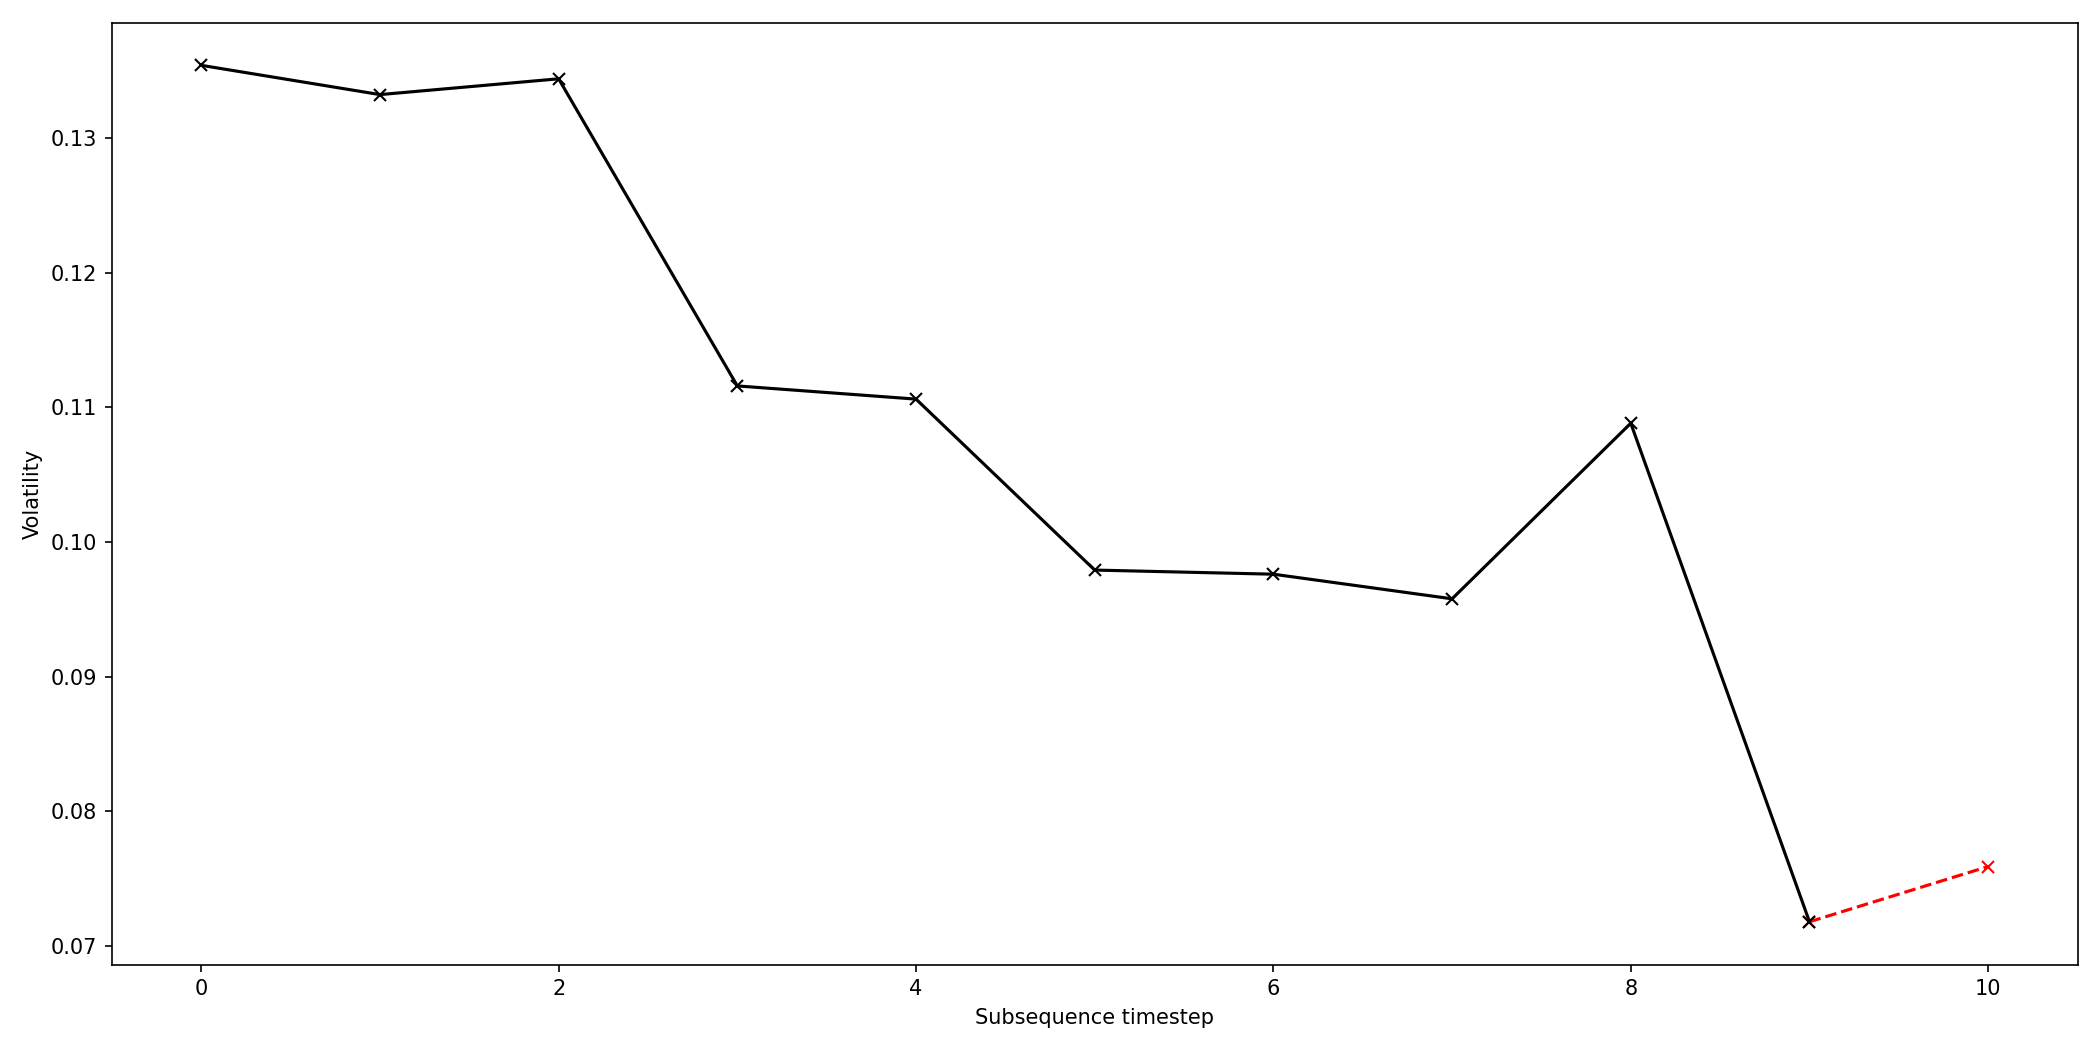
\includegraphics[width=0.5\textwidth]{volatility-subsequence.png}
        \caption{\centering Volatility subsequence for an example data instance, including the true label.}
        \label{fig: volatility-subsequence}
    \end{figure}


    This multivariate, time windowed approach was chosen as it has been effectively used by a host of popular studies on the use of DNNs for time series prediction, and in particular volatility forecasting. For example, \citet{xiong-2016} used $25$-dimensional multivariate time series (including daily open, close, high, and low prices, and returns) to demonstrate the prediction accuracy and robustness of their RNN for the S\&P 500. Furthermore, \citet{xiong-2016}, \citet{bucci-2020}, and \citet{rodikov-2022} all utilised a dataset consisting of time windowed subsequences; \citet{xiong-2016} specifically made predictions using a $10$-step rolling time window, as they found this to be consistent with the majority of comparable models in this field. Hence, a dataset has been developed in keeping with popular modelling implementations within this field.


    \section{Analysis Approach}
    \label{section: metrics}

    To demonstrate the performance and efficiency of each training algorithm, after each DNN had finished training it was tested over the testing dataset $D_{test}$, constructed by implementing a train-test split of the full dataset $D$, partitioning it into two distinct subsets $D_{train}$ and $D_{test}$. In this research, an $80 \colon 20$ split is implemented, using $80\%$ of data instances for training and the remaining $20\%$ for testing (determined experimentally to produce the best results).
    
    % this split is demonstrated for the full (unwindowed) volatility time series in Figure \ref{fig: traintest-split}.


    % \begin{figure}[ht]
    %     \centering
    %     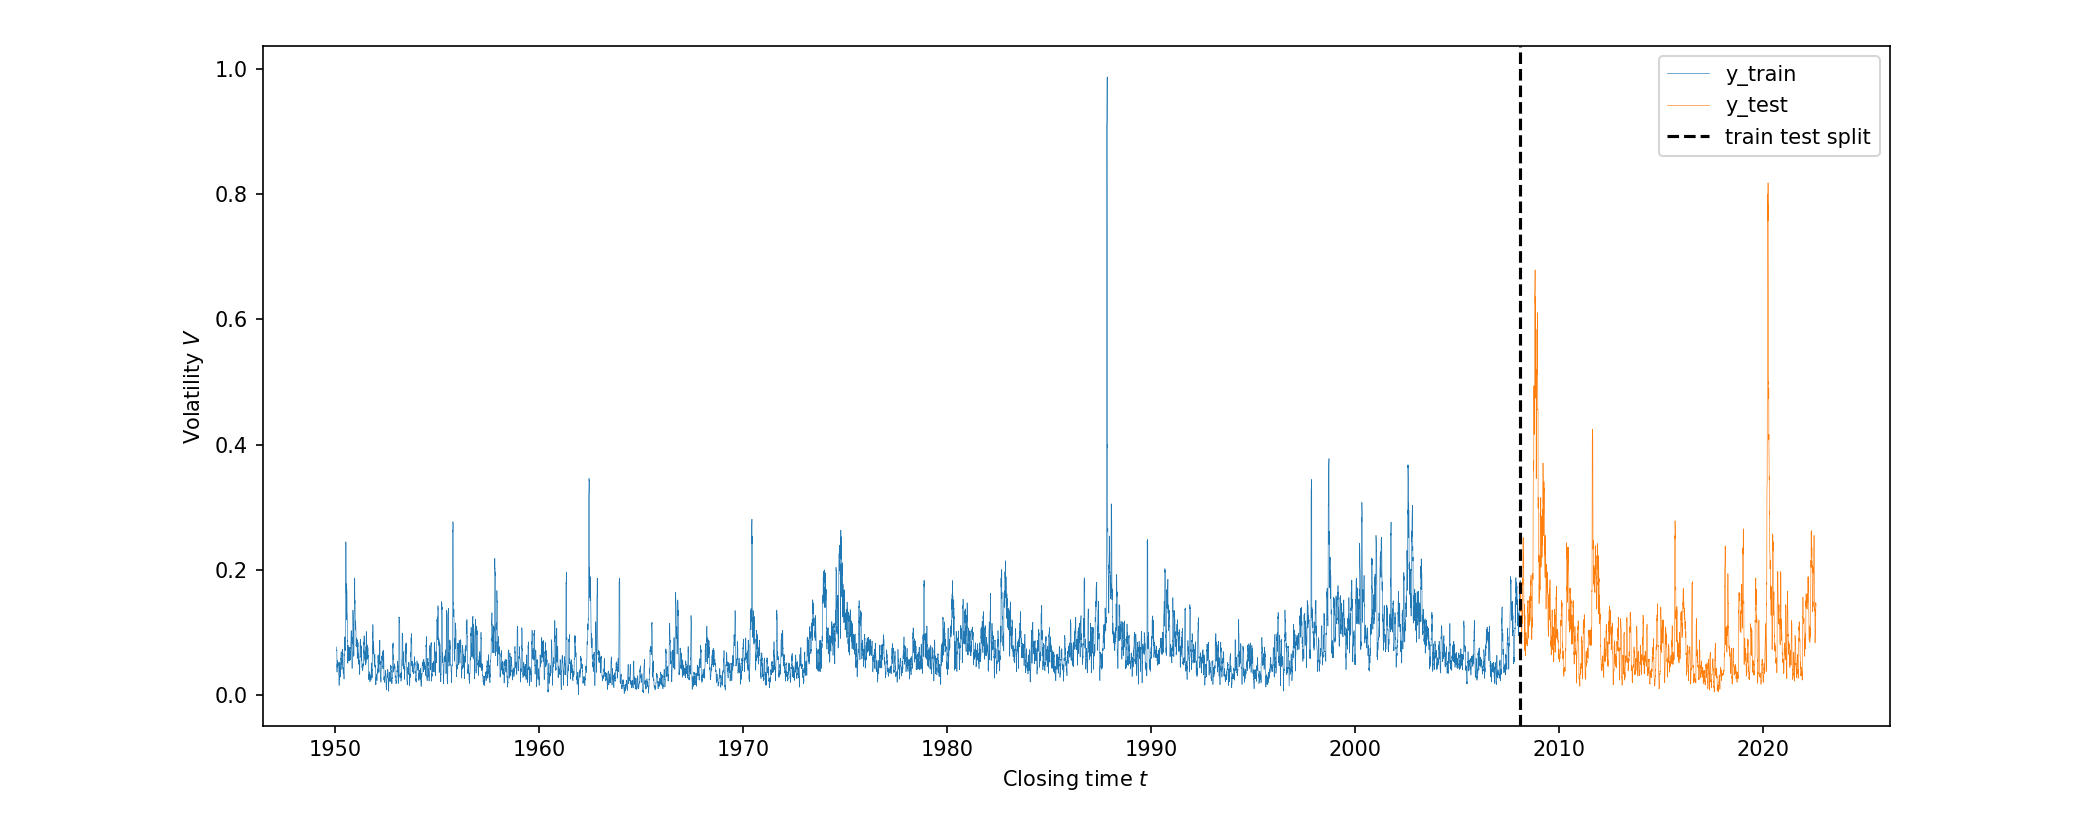
\includegraphics[width=0.7\textwidth]{traintest-split.png}
    %     \caption{\centering Visualisation of the train-test split dividing training (blue) and testing (orange) data.}
    %     \label{fig: traintest-split}
    % \end{figure}


    \subsection{Accuracy Metrics}
    \label{section: accuracy-metrics}

    After training, the DNNs predictions over $D_{test}$ are analysed through statistical metrics that quantify the modelling error $\varepsilon$ and prediction accuracy. These accuracy metrics measure the divergence between the predicted volatility time series value $\hat{y}_t = \hat{v}_{t+1}$ and the true label $y_t = v_{t+1}$. These metrics are important as they demonstrate the success of all training algorithms, contextualising the forecasting performance generated by each approach.

    One metric commonly used to quantify forecasting performance is the \emph{coefficient of determination} $R^2$ \citep{zhang-2022}, which computes the ratio between the estimated variance of the prediction error $\varepsilon$ and the variance of the variable $y_t$ being predicted, shown in Equation \ref{eq: r-squared} for the predictions $\hat{y}_t$ (and sample mean of labels $\mu_{y}$). The value of $R^2$ for a given set of predictions represents the proportion of the variability in the label set that is correctly captured by the model's predictions; it ranges between $- \infty$ and $1$, with a score of $1$ meaning the true labels have been perfectly represented. This an effective metric for demonstrating how well a model represents data, and has been used to showcase the performance of several volatility models such as the ANN implementation of \citet{zhang-2022}. However, it also has several limitations. Most notably, this metric doesn't explicitly quantify whether a model is good or bad, it only shows whether the testing performance is noticeably better than that of a comparison \emph{constant model} that outputs predictions simply as the sample mean of the observed inputs; hence, its results can sometimes be misleading.


    \begin{equation}
        \label{eq: r-squared}
        R^2 = 1 - \frac{\sum_{t=0}^n (y_t - \hat{y}_t)^2}{\sum_{t=0}^n (y_t - \mu_{y}))^2}
    \end{equation}


    Because of this limitation, several other statistical metrics are commonly used to quantify the prediction accuracy of DNNs. Two such measures are the \emph{mean absolute error} (MAE) and \emph{root mean squared error} (RMSE). Given the set of predictions $\hat{y}_t$ and labels $y_t$, MAE measures the average magnitude of the prediction error $\varepsilon$, taken as the mean absolute difference between $\hat{y}_t$ and $y_t$ over the entire test set (Equation \ref{eq: mae}). RMSE also measures the magnitude of deviations, computing this as the standard deviation of prediction errors (Equation \ref{eq: rmse}). Low MAE and RMSE (close to $0$) both indicate that the model is accurate; however, the squared component of RMSE gives increasing weight to large errors and hence is useful for penalising highly anomalous predictions more than slight deviations, whereas MAE gives a uniform representation of $\varepsilon$. One limitation of both MAE and RMSE is that they are scale-dependent; when predicting small values the magnitude of the calculated error will always be smaller than that generated predicting large values, irrespective of the model's accuracy. Hence, these metrics are typically utilised to compare various models over the same domain, such as by \citet{rodikov-2022} who used both MAE and RMSE to compare the performance of LSTMs and GARCH. The MAE and RMSE accuracy metrics will be used similarly in the research of this thesis, comparing the performance of the traditionally trained DNN to the DNNs using energy and data-efficient training algorithms. 


    \begin{equation}
        \label{eq: mae}
        MAE = \frac{1}{n} \sum_{t=0}^n \lvert y_t - \hat{y}_t \lvert
    \end{equation}
    
    \begin{equation}
        \label{eq: rmse}
        RMSE = \sqrt{\frac{1}{n} \sum_{t=0}^n (y_t - \hat{y}_t)^2}
    \end{equation}


    To further quantify the accuracy of the implemented models, and address the inherent issues of preceding measurements, a scale-independent measure is required. One such metric is the \emph{mean absolute percentage error }(MAPE) of predictions, which computes the absolute difference between $\hat{y}_t$ and $y_t$ over the test set as a percentage average (Equation \ref{eq: mape}). This provides an objective and easily interpretable picture of the accuracy of a model and has been used to analyse numerous volatility forecasting DNNs, including by \citet{xiong-2016} and \citet{zhang-2022}. Hence, this research additionally computes the MAPE of each implementation to independently demonstrate the performance of each trained model.


    \begin{equation}
        \label{eq: mape}
        MAPE = \frac{1}{n} \sum_{t=0}^n \bigg\lvert \frac{y_t - \hat{y}_t}{y_t} \bigg\lvert * 100\%
    \end{equation}


    \subsection{Efficiency Metrics}
    \label{section: efficiency-metrics}

    Beyond generating accurate performance, the efficiency of each training algorithm is of vital importance to this research. Several efficiency metrics have been presented by \citet{schwartz-2019}, who assert that the computational cost of a DNN is proportional to the cost of passing a single data instance through the network, the size of the utilised datasets, and the number of hyperparameters being tuned (Equation \ref{eq: cost-r}). Since the architecture used in this research is fixed, and the hyperparameters predetermined, these variables are not covered by the efficiency calculations analysed; however, dataset size is inspected for data-efficient training algorithms.

    \citet{amodei-2018} also explore the efficiency of DNN training, asserting that the cost of a training algorithm is dependent on the utilised hardware and training time. As the implemented studies all use the same hardware, metrics that target hardware efficiency are redundant to this research. However, training time is an important aspect of computational cost, and hence to quantify energy efficiency the total time required to train a DNN with accurate performance is recorded. Training time is a simple but effective efficiency metric, as more time typically means a higher computational cost. Although it is important to note that training time is not a completely representative metric, as it is reliant upon the underlying hardware and software dependencies of the system \citep{schwartz-2019}. However, since this efficiency metric is used for comparison of the relative differences in efficiency between implementations (all of which use the same underlying hardware and software), the calculation of training time is both valid and beneficial in this context.

    The efficiency of a training algorithm can additionally be determined by inspecting how fast and smoothly the minimum of the loss function is converged upon. As outlined in Section \ref{section: deep-learning}, a DNN is trained by adjusting the network's parameter set in the direction of the negative gradient of the loss function, determined through backpropagation of the DNN's prediction error. Hence, the purpose of DNN training is to find the optimal parameter set that corresponds to the minimum of that loss function. The efficiency of a DL training process can therefore be determined by the speed at which this minimum point is approached; this is known as the \emph{convergence rate} of training, which calculates the size of the step taken towards the loss function's minimum during each epoch. Convergence rate is an important factor when considering the efficiency of a DL training algorithm, as the faster a DNN's parameters converge towards their optimal values, the more effective the early stages of training (as the DNN learns more over each epoch), and thus the less time, fewer calculations, and lower energy consumption is required to develop an accurate model. Hence, convergence rate is also evaluated to demonstrate the efficiency of each training algorithm.


    \section{Baseline Model Implementation}
    \label{section: baseline}

    Before analysing the efficiency of each training algorithm, a model architecture characteristic of those used in Fintech must be implemented. This should ensure that the findings of this research are universal, demonstrating on a wide scale how the ESG impacts of DL for finance can be mitigated.
    

    \subsection{Baseline Volatility Forecasting Model}
    \label{section: model-architecture}

    To conduct volatility forecasting, an LSTM architecture was chosen, as RNNs are proven to produce superior forecasting accuracy over time series, accurately modelling both long and short-term dependencies in sequences, and capturing complex dependencies between highly variable features. Furthermore, they have been successfully applied to forecasting financial market volatility, with \citet{bucci-2020} showing that LSTMs outperform traditional volatilty forecasting models.

    The hyperparameters regulating the number of hidden layers and neurons per layer within the DNN were then determined, constructing a hyperparameter set representative of typical models in this field. Existing models in literature were found to typically exploit between $1$ \citep{bucci-2020} and $5$ \citep{kim-2018} layers; therefore, to strike a balance between these implementations the implemented model relies on $3$ LSTM layers, each containing $24$ neurons (Table \ref{table: architecture}). Since the output layer is used to return a single prediction $\hat{v}_{t+1}$, this layer contains a single neuron fully-connected to its preceding hidden layer, from which the network's single output value is read.


    \begin{table}[ht]
        \centering
        \begin{tabular}{|l|l|l|l|} 
        \hline
        \textbf{\footnotesize Layer} & \textbf{\footnotesize Type} & \textbf{\footnotesize Output Shape}   & \textbf{\footnotesize Parameter Count}  \\ 
        \hline
        Input layer    & Vector        & $(32, 10, 7)$  & -                         \\ 
        \hline
        Hidden layer 1 & LSTM          & $(32, 10, 24)$ & 3072                      \\ 
        \hline
        Hidden layer 2 & LSTM          & $(32, 10, 24)$ & 4704                      \\ 
        \hline
        Hidden layer 2 & LSTM          & $(32, 10, 24)$ & 4704                      \\ 
        \hline
        Output layer   & Fully-connected           & $(32, 1)$      & 25                        \\
        \hline
        \end{tabular}
        \caption{\centering Architecture of the LSTM model implementation.}
        \label{table: architecture}
    \end{table}


    \subsection{Baseline Training Algorithm}

    To train the DNN within this initial study, a baseline training algorithm was implemented using backpropagation and gradient descent. The model (with aforementioned architecture) was trained over a specified number of iterations over the full dataset (each iteration is known as an \emph{epoch}), within which batches of data are sampled and input into the model. Before training could commence, the algorithm's \emph{learning rate}, \emph{epoch count}, and \emph{batch size} hyperparameters had to be determined. The surveyed models typically used a learning rate of $0.001$ \citep{zhang-2022}, trained over between $50$ \citep{rahimikia-2020} and $600$ \citep{xiong-2016} epochs, and sampled data in batches of size $32$ \citep{xiong-2016}. Hence, to implement a model that was both characteristic of these statistics and experimentally determined to produce the best performance, a learning rate of $0.001$, epoch count of $100$, and batch size of $32$ were chosen (Table  \ref{table: hyperparams}).

    \begin{table}[ht]
        \centering
        \begin{tabular}{|l|l|l|l|l|l|l|l|} 
            \hline
            \begin{tabular}[c]{@{}l@{}}\textbf{\footnotesize Window}\\\textbf{\footnotesize Size}\end{tabular} & \begin{tabular}[c]{@{}l@{}}\textbf{\footnotesize Time Series}\\\textbf{\footnotesize Variables}\end{tabular} & \begin{tabular}[c]{@{}l@{}}\textbf{\footnotesize Prediction}\\\textbf{\footnotesize Length}\end{tabular} & \textbf{\footnotesize Layers} & \textbf{\footnotesize Neurons} & \begin{tabular}[c]{@{}l@{}}\textbf{\footnotesize Learning}\\\textbf{\footnotesize Rate}\end{tabular} & \textbf{\footnotesize Epochs} & \begin{tabular}[c]{@{}l@{}}\textbf{\footnotesize Batch}\\\textbf{\footnotesize Size}\end{tabular}  \\ 
            \hline
            10                                                                      & 7                                                                                 & 1                                                                             & 3               & 24               & 0.001                                                                     & 100             & 32                                                                     \\
            \hline
        \end{tabular}

        \caption{\centering Hyperparameters of baseline model implementation and training algorithm.}
        \label{table: hyperparams}
    \end{table}


    \section{Summary}

    Hence, a financial volatility forecasting model was developed over the S\&P 500 market using a 3-layer LSTM architecture. This model is trained over $100$ epochs, recording the efficiency of training to give an insight into the computational cost of traditional DL algorithms, and contextualise the performance and efficiency of the efficient algorithms implemented later in this research.


    \chapter{Energy-Efficient Training Algorithms}
    \label{chapter: energy-extensions}

    \section{Aims of Study}

    Building upon the baseline approach, energy-efficient training algorithms are explored that minimise the energy expended training a volatility forecasting DNN. This research focuses on three avenues through which the training process of a DNN can be adapted to improve energy efficiency: mixed-precision training, supervised layer-wise pre-training, and unsupervised layer-wise pre-training. These implementations all use the same dataset and model architecture presented in Chapter \ref{chapter: experiments}. Initially, mixed-precision training is implemented, where network computations are quantised to utilise low-bit representations. This exploration aims to demonstrate how using lower precision variables can boost training speed whilst still producing an accurate model, thus showing that mixed-precision training is a viable mechanism for reducing the energetic cost of developing DNNs in finance. The experimentation then proceeds to explore progressive training methods; this begins by implementing a supervised pre-training process, that additionally aims to reduce traiing time and energy consumption. Unsupervised pre-training is then explored, where a more complex approach is taken to pre-train the proposed DNN to produce further computational cost reductions.


    \section{Mixed-Precision Training Algorithm}
    \label{section: mixed-precision-method}

    The first method presented by this research for reducing the energy consumption of DL is mixed-precision training. As explored in Section \ref{section: quantisation-training}, quantisation is often used within Green AI to reduce resource requirements. These implementations reduce energy and memory costs by lowering the precision at which variables are stored and operations are evaluated \citep{fan-2020b}. In real-world applications, quantisation is often realised through mixed-precision training, where a combination of high-precision and quantised representations are used to balance efficiency and accuracy \citep{ott-2017}. This research aims to demonstrate how mixed-precision training can be used to reduce the computational and memory cost of training DNNs, mitigating the energy consumption and ESG impacts of DL in finance.

    To implement mixed-precision training, the \emph{Keras mixed-precision API} \citep{abadi-2016} was exploited. This API enables ML developers to adapt the precision of variables and operations within an implemented DNN, changing the default $32$-bit precision. In this research, the mixed precision API is used to specify a \emph{`mixed\_float16'} precision policy \citep{abadi-2016}, where a combination of $16$-bit and $32$-bit floating-point data types are used during training. Specifically, this exploits $16$-bit floating-point variables for evaluating network computations, whilst maintaining a $32$-bit floating-point representation for storage. Using lower precision reduces the amount of memory used by network operations, increasing the speed of calculations and reading from memory by minimising their computational load and allowing increased hardware acceleration. Specifically, $16$-bit representations are utilised as modern GPUs and TPUs have been shown to run operations significantly faster when using $16$-bit precision, as batches of data consume half the amount of memory when being passed through the DNN. High precision is still used for storing variables to maintain numerical stability, ensuring that the model maintains accurate performance. Hence, this implementation of mixed-precision training strikes a compromise between reducing the energetic cost of network operations during training and preserving accurate performance.

    The efficiency of mixed-precision training was evaluated by using the same DNN as proposed in Section \ref{section: baseline}. First, the use of a `mixed\_float16' precision policy is specified; an identical network with the same LSTM-based architecture and hyperparameters of the baseline model (Tables \ref{table: architecture} and \ref{table: hyperparams}) is then implemented using variables of the specified precision. This DNN is trained using the same training algorithm as in the baseline case, for the same number of epochs.


    \section{Supervised Layer-wise Pre-Training Algorithm}

    Pre-training is also a popular approach within Green AI, which aims accurate models to be developed more intelligently and efficiently. Progressive training is one such pre-training method, highlighted by Green AI researchers (such as \citet{xu-2021}) as being capable of reducing the length of DNN training through a computationally inexpensive pre-training phase. As discussed in Section \ref{section: progressive-training}, progressive training constructs a DNN layer-by-layer through an iterative process of adding new layers and training each individually. Research into this approach---such as the exploration of \citet{ienco-2019}---has shown its effectiveness at reducing the computational cost of training a DNN, as the inexpensive pre-training phase (which is computationally cheap since only single network layers are trained) allows a significant reduction in the number of epochs necessary to optimise the parameters of the full network. Both the low-cost pre-training phase and shortened full network training mean that progressive training is an effective way to reduce training time and energy consumption, providing a promising avenue for improving the ESG impact of DL in finance.

    In this study, supervised layer-wise pre-training will be explored to demonstrate the benefits of progressive training. This method individually trains network layers through supervised learning over a labelled dataset outlining the modelling task \citep{ienco-2019}. In our case, the time series dataset outlined in Section \ref{section: dataset} is used, with each round of pre-training optimising a new layer's parameters to predict the HV $\hat{v}_{t+1}$ at timestep $t+1$ within a sequence. In this research, the base model at the start of pre-training consists of a single LSTM layer combined with a fully-connected single-neuron output layer. To execute the training algorithm, each pre-training round (where a single layer is added and optimised) was conducted over $20$ epochs. A further $30$ epochs were then used to conclude training, where the parameters of the full network are tuned. This proportion of pre-training and tuning epochs was chosen  to provide the best accuracy-efficiency tradeoff, minimising the total length of training but maintaining the model's forecasting performance. 

    The first pre-training round focuses on training the base network. This shallow network is trained over the dataset $D_{train}$, optimising the parameters of the single LSTM layer and the DNN's output layer. After $20$ epochs, the parameters of the first layer are fixed, a new LSTM layer is added between the initial hidden layer and the output layer, and another $20$ pre-training epochs are executed. This iterative process was repeated until a DNN with $3$ LSTM layers was constructed, meaning this experimentation utilised the same architecture as in the baseline case. After the full network is pre-trained, final tuning begins, where all network parameters are unfixed and optimised over $20$ additional epochs, starting from the initialisation values deduced during pre-training.


    \section{Unsupervised Layer-wise Pre-Training Algorithm}

    Although supervised layer-wise pre-training is a simple method through which progressive training can be realised, greater performance and efficiency can be achieved through unsupervised layer-wise pre-training. Both \citet{xu-2018} and \citet{sagheer-2019} found this approach induced faster convergence toward the optimal parameter set and smaller prediction error than traditional training algorithms. Hence, in an attempt to further improve the efficiency of DNN training in the chosen domain, an unsupervised layer-wise pre-training algorithm is also implemented.

    Unsupervised layer-wise pre-training similarly begins by initialising a single-layer base network. The base architecture was identical that used in the supervised case, except the output layer which used a different structure to enable unsupervised learning. This output layer consisted of the same dimensions as the input layer such that the network could be trained as an autoencoder. Since the same training dataset of multivariate time series subsequences was utilised, the unsupervised pre-training approach trained each layer to reconstruct this subsequence, meaning the network learned to output a representation of the input time series (tuning its parameters to minimise the difference between each layer's inputs and outputs). Layer-wise pre-training was then implemnted, optimising each LSTM layer independently as an autoencoder over $7$ epochs to result in a 3-layer DNN. The concluding full network tuning stage over $50$ epochs then converts this autoencoder into a forecasting model that predicts the volatility $\hat{v}_{t+1}$ based upon each input time series. To achieve this, the autoencoder output layer is discarded and replaced by a single fully-connected output neuron, which is optimised (alongside the three hidden layers) over the tuning stage.


    \section{Summary}

    Hence, to demonstrate how Green AI can improve the energy efficiency of training DL models in finance, three algorithms were implemented: mixed-precision training, supervised layer-wise pre-training, and unsupervised layer-wise pre-training. To evaluate the success of each method, a DNN with the same architecture as presented in Section \ref{section: model-architecture} was trained, recording the efficiency of the training process and the accuracy of the resulting model. This involved the calculation of the $R^2$, MAE, RMSE, and MAPE of test predictions, to deduce the accuracy of each developed model, and quantify the performance difference to the baseline model. The total training time and convergence rate were also recorded over the execution of each algorithm, which are then put into context against those computed for the baseline model, demonstrating the efficiency gains of the new model, and exemplifying the benefit of the adapted training algorithms for reducing the energy consumption, carbon emissions, and ESG impacts of DL-based financial volatility forecasting models.


    \chapter{Data-Efficient Training Algorithms}
    \label{chapter: data-extensions}

    \section{Aims of Study}

    A core component of the computational cost of cutting-edge DL algorithms is the use of extremely large dataset, which force performance gains through training a model over expanses of data, most of which is not beneficial to learning \citep{bender-2021}. Whilst this has been shown to facilitate impressive accuracy, current DNNs typically do not deal with data intelligently or efficiently \citep{aljarrah-2015}; this is because a significant amount of time and energy is wasted training over redundant data instances that do not benefit performance, accruing an alarming energetic cost.

    Therefore, this research explores data-efficient training algorithms that minimise training data requirements, further improving the efficiency of training and minimising memory and energy costs. Specifically, active learning is employed, which adapts the training process to intelligently select data instances that are the most beneficial to learning, discarding redundant instances. Thus, the training dataset size is reduced, lowering the time and energy expended during training. 

    Furthermore, \citet{bender-2021} showed that compact networks with small parameter sets typically require increased amounts of training data to achieve comparable performance to larger models. Thus, data-efficient training algorithms additionally allow compact networks to be used without inflicting the further computational costs associated with large datasets.


    \section{Active Learning Algorithm}
    \label{section: al-model}

    As described in Section \ref{section: active-learning}, active learning has been shown to drastically improve the data efficiency of training DNNs by reducing the time and energy wasted on redundant data instances \citep{xu-2021}, as well as achieving an exponential improvement in the time required to label training data, and successfully dealing with high-dimensional sequential data \citep{ren-2021}. The active learning training process implemented in this research aims to reduce computational costs by training over a subset of the data space containing instances believed to provide the most utility to the model's learning process. In this experimentation, pool-based active learning is implemented, which uses two datasets $P \subset D_{train}$ and $V \subseteq D_{train}$ to split useful and unuseful data according to an importance function. Beginning with an initial seed $P^{(1)}$ of $n_{sample}$ instances, an iterative process is exploited where the DNN is trained over pool $P$ and used to predict the outputs of all data instances in the validation set $V$; these predictions are then evaluated through the importance function, and the $n_{sample}$ most important data instances moved into the pool before the next training round is conducted.

    In this research, data instances are selected through two algorithms known as \emph{greedy sampling on the inputs} (GSx) and \emph{greedy sampling on the outputs} (GSy). These methods, conceived by \citet{wu-2019}, implement a performant greedy sampling approach that aims to increase the diversity of the input and output spaces of a model, improving training efficiency. In our implementation, GSx is used to specify the initial seed pool $P^{(1)}$, and GSy is used in the following training iterations to select data instances to be moved from the validation set $V^{(i)}$ to the pool set $P^{(i+1)}$. 

    GSx \citep{wu-2019} is an algorithm for constructing the seed pool $P^{(1)}$ by selecting $n_{sample}$ data instances from the full dataset $V^{(0)} = D_{train}$ of size $N$ \citep{wu-2019}. Firstly, GSx selects the single data instance from the full validation set $V^{(0)}$ that is the shortest distance from the dataset's mean instance; in this case, the \emph{Euclidean distance} is used. Once the data instance closest to the dataset's mean is found, it moved from $V^{(0)}$ to $P^{(1)}$. This value is then used to iteratively find the remaining $n_{sample} - 1$ instances; to find instance $x_i$, we first compute the Euclidean distance between each data instance $x_m$ already in the seed pool and each instance $x_n$ remaining in $V^{(0)}$, constructing a 2D distance matrix (Equation \ref{eq: GSx-distance}). Then, for each instance $x_n$ remaining in $V^{(0)}$ we select the corresponding seed value $v_m$ that minimises the distance $x_n \to x_m$, building a 1D distance vector enumerating the closest seed instance to each remaining validation set element (Equation \ref{eq: GSx-min}). Finally, the data instance $x_n$ furthest from all existing seeds (i.e. the maximum of the distance vector) is selected and moved from $V^{(0)}$ into $P^{(1)}$. This process is repeated until we have a full seed $P^{(1)}$ of $n_{sample}$ data instances, and a validation set $V^{(1)}$ of $N - n_{sample}$ instances. By adding seeds that are furthest from any others in the pool, GSx ensures that the seed pool used to initially train the DNN is as diverse in the data space as possible, giving the model a complete picture of the breadth of the full training dataset whilst only using a small subset of instances.


    \begin{equation}
        \label{eq: GSx-distance}
        d^{(x)}_{n, m} = \lVert x_n - x_m \lVert
    \end{equation}
  
    \begin{equation}
        \label{eq: GSx-min}
        d^{(x)}_n = \min_m d^{(x)}_{n, m}
    \end{equation}


    GSy \citep{wu-2019} aims to capture diverse instances from the output space of the model $M_{\theta}$ that realises the function $y = f( x \vert \theta )$ \citep{wu-2019}. The GSy algorithm implements an iterative approach where data instances are selected from the validation set $V^{(i)}$ to add to the pool $P^{(i+1)}$ such that the prediction error of the function $f( x \vert \theta )$ over the total dataset is minimised. Namely, when considering an input instance $x_n$, if the model produces an output $y_n = f( x_n \vert \theta )$ that is noticeably distinct from the outputs generated from other data instances, the algorithm selects $x_n$ to add to the training pool as it helps refine the parameters defining the model's predictions. GSy then works by the assertion that the more diverse the pool instances $x_m$ collected, the more accurately the optimal parameters of the model can be determined. However, this algorithm requires a functioning model $f( x \vert \theta )$ to exist (such that model outputs can be generated and analysed), so it can only be used to populate a pool that has already been initialised with seed instances. Therefore, \citet{wu-2019} assert that to implement active learning, GSx should be used for determining the seed, followed by GSy to further populate the pool set at later training iterations.

    Given a pool $P^{(1)}$ of $n_{sample}$ data instances, and validation set $V^{(1)}$ of $N - n_{sample}$ instances, the GSy algorithm selects $n_{sample}$ instances to move from $V^{(1)}$ to form the new datasets $P^{(2)}$ and $V^{(2)}$ believed to provide the most utility to training. This is done by first evaluating the model $f( x_n \vert \theta )$ over all data instances $x_n \in V^{(1)}$, to create the set of predicted labels $\hat{Y}^{(1)} = \{ \hat{y}_n \colon \hat{y}_n = f( x_n \vert \theta ) \forall x_n \in V^{(1)} \}$. Once all $N - n_{sample}$ predicted labels have been computed over the validation set $V^{(1)}$, a 2D distance matrix is constructed enumerating the distance (as the absolute difference) between each prediction $\hat{y}_n$ and all true labels $y_m$ of the data instances $x_m$ that already exist within the pool set $P^{(1)}$ (Equation \ref{eq: GSy-distance}). From the distance matrix a 1D distance vector is constructed over the $N - n_{sample}$ outputs of the validation set $V^{(1)}$, enumerating the shortest distance of each prediction $\hat{y}_n$ to a true label $y_m$ of an instance $x_m$ in the pool set (Equation \ref{eq: GSy-min}). The data instances in the validation set corresponding to the $n_{sample}$ largest distances in the distance vector are then selected and moved from the validation set to the pool, creating the new datasets $P^{(2)}$ and $V^{(2)}$. This process is repeated at each training round, allowing the pool to be iteratively populated with data instances that stimulate diverse outputs from the model being trained. Thus, a DNN is developed that can produce a wide range of appropriate outputs to accurately represent a spectrum of different predictions (allowing the DNN to model a plethora of different possible scenarios), despite only being trained over a limited number of data instances.


    \begin{equation}
        \label{eq: GSy-distance}
        d^{(y)}_{n, m} = \lvert \hat{y}_n - y_m \lvert = \lvert f( x_n \vert \theta ) - y_m \lvert
    \end{equation}
  
    \begin{equation}
        \label{eq: GSy-min}
        d^{(y)}_n = \min_m d^{(y)}_{n, m}
    \end{equation}


    In their research, \citet{wu-2019} found that GSx and GSy improved the data efficiency of training and produced a model that exhibits impressive generalisability when compared to approaches using random sampling to select data instances. This demonstrates the effectiveness and robustness of active learning training that uses GSx and GSy. Hence, the experimentation into data-efficient training for DNNs presented in this thesis utilises GSx for picking the seed pool of $n_{sample} = 100$ data instances and GSy at each following training iteration $i$ to select a further $100$ data instances to move into the pool set. The full $3$-layer DNN proposed in Section \ref{section: baseline} is utilised over this iterative process, training over the expanding pool set for $100$ training rounds.


    \section{Summary}

    Hence, to exemplify DNNs can be trained in a data-efficient manner in financial domains, an active learning algorithm was implemented, initially selecting a seed pool using the GSx algorithm and iteratively building up the training dataset through the GSy algorithm \citep{wu-2019}. To evaluate the performance and efficiency of this training algorithm, a comparative analysis is conducted between the baseline algorithm and the active learning implementation. A close inspection of the amount of data utilised over training is made, demonstrating how active learning can reduce the data requirements of training DNNs within the chosen financial domain. Whilst proposing the GSx and GSy algorithms, \citet{wu-2019} raise several limitations of this approach; they found that when the pool size during the early stages of training is too small the model being built exhibits very high variance, meaning its performance is not reliable. Therefore, inspecting the convergence rate of the DNN's parameters over training (to show the stability of training) is essential to exploring benefits and drawbacks of active learning for improving the efficiency of DNN training.


    % --------------------  EVALUATION ----------------------
    \newpage
    \chapter{Results \& Discussion}
    \label{chapter: results-discussion}

    The following chapter explores the results of the presented studies. Initially, the data collected from each experiment is presented, summarising what is shown by the research findings, highlighting their significance, and examining their implications for the research hypotheses. Once all results have been outlined, a detailed discussion surrounding the success of each experiment is undertaken, evaluating how effective Green AI approaches are at reducing the computational cost of DNN training within the chosen application of financial volatility forecasting. The results of each experiment are presented and discussed with close reference to the accuracy and efficiency measures introduced in Section \ref{section: metrics}, quantifying both the performance and efficiency of each approach.
    
    Each result was derived by tuning the hyperparameters of each training algorithm to maximise model accuracy whilst maintaining an efficiency greater than that of the baseline training approach. This prioritised developing models with low prediction error, then evaluated the efficiency of the training process exploited to develop that model. To evaluate each training algorithm in a robust and reproducible manner, each was employed five times, optimising a model from scratch over a fixed number of epochs; the results of the most successful training round were then collected as the outcome of this research. This was to ensure that a representative result of the true ability of each training algorithm was obtained and that the outcome of this research was not biased or degraded by the stochastic nature of DL training algorithms, which can cause results to vary over different executions. To ensure reproducible and generalisable results, the model and training process is implemented in \emph{Python} with the popular DL framework \emph{TensorFlow} \citep{abadi-2016}. The implementations were run on \emph{Google Colaboratory Pro} to achieve higher training performance by exploiting high-end ML hardware, executing each algorithm using a \emph{Tesla T4} GPU. 

    \section{General Predictive Performance}

    To demonstrate the success of each algorithm, each trained model was employed to forecast volatility over the test dataset. Figure \ref{fig: predictions} shows the forecasts of all models, showcasing the predicted volatilities $\hat{v}_{t+1}$ over all timesteps of the testing period, contextualised against the true values $v_{t+1}$.


    \begin{figure}[ht!]
        \centering
        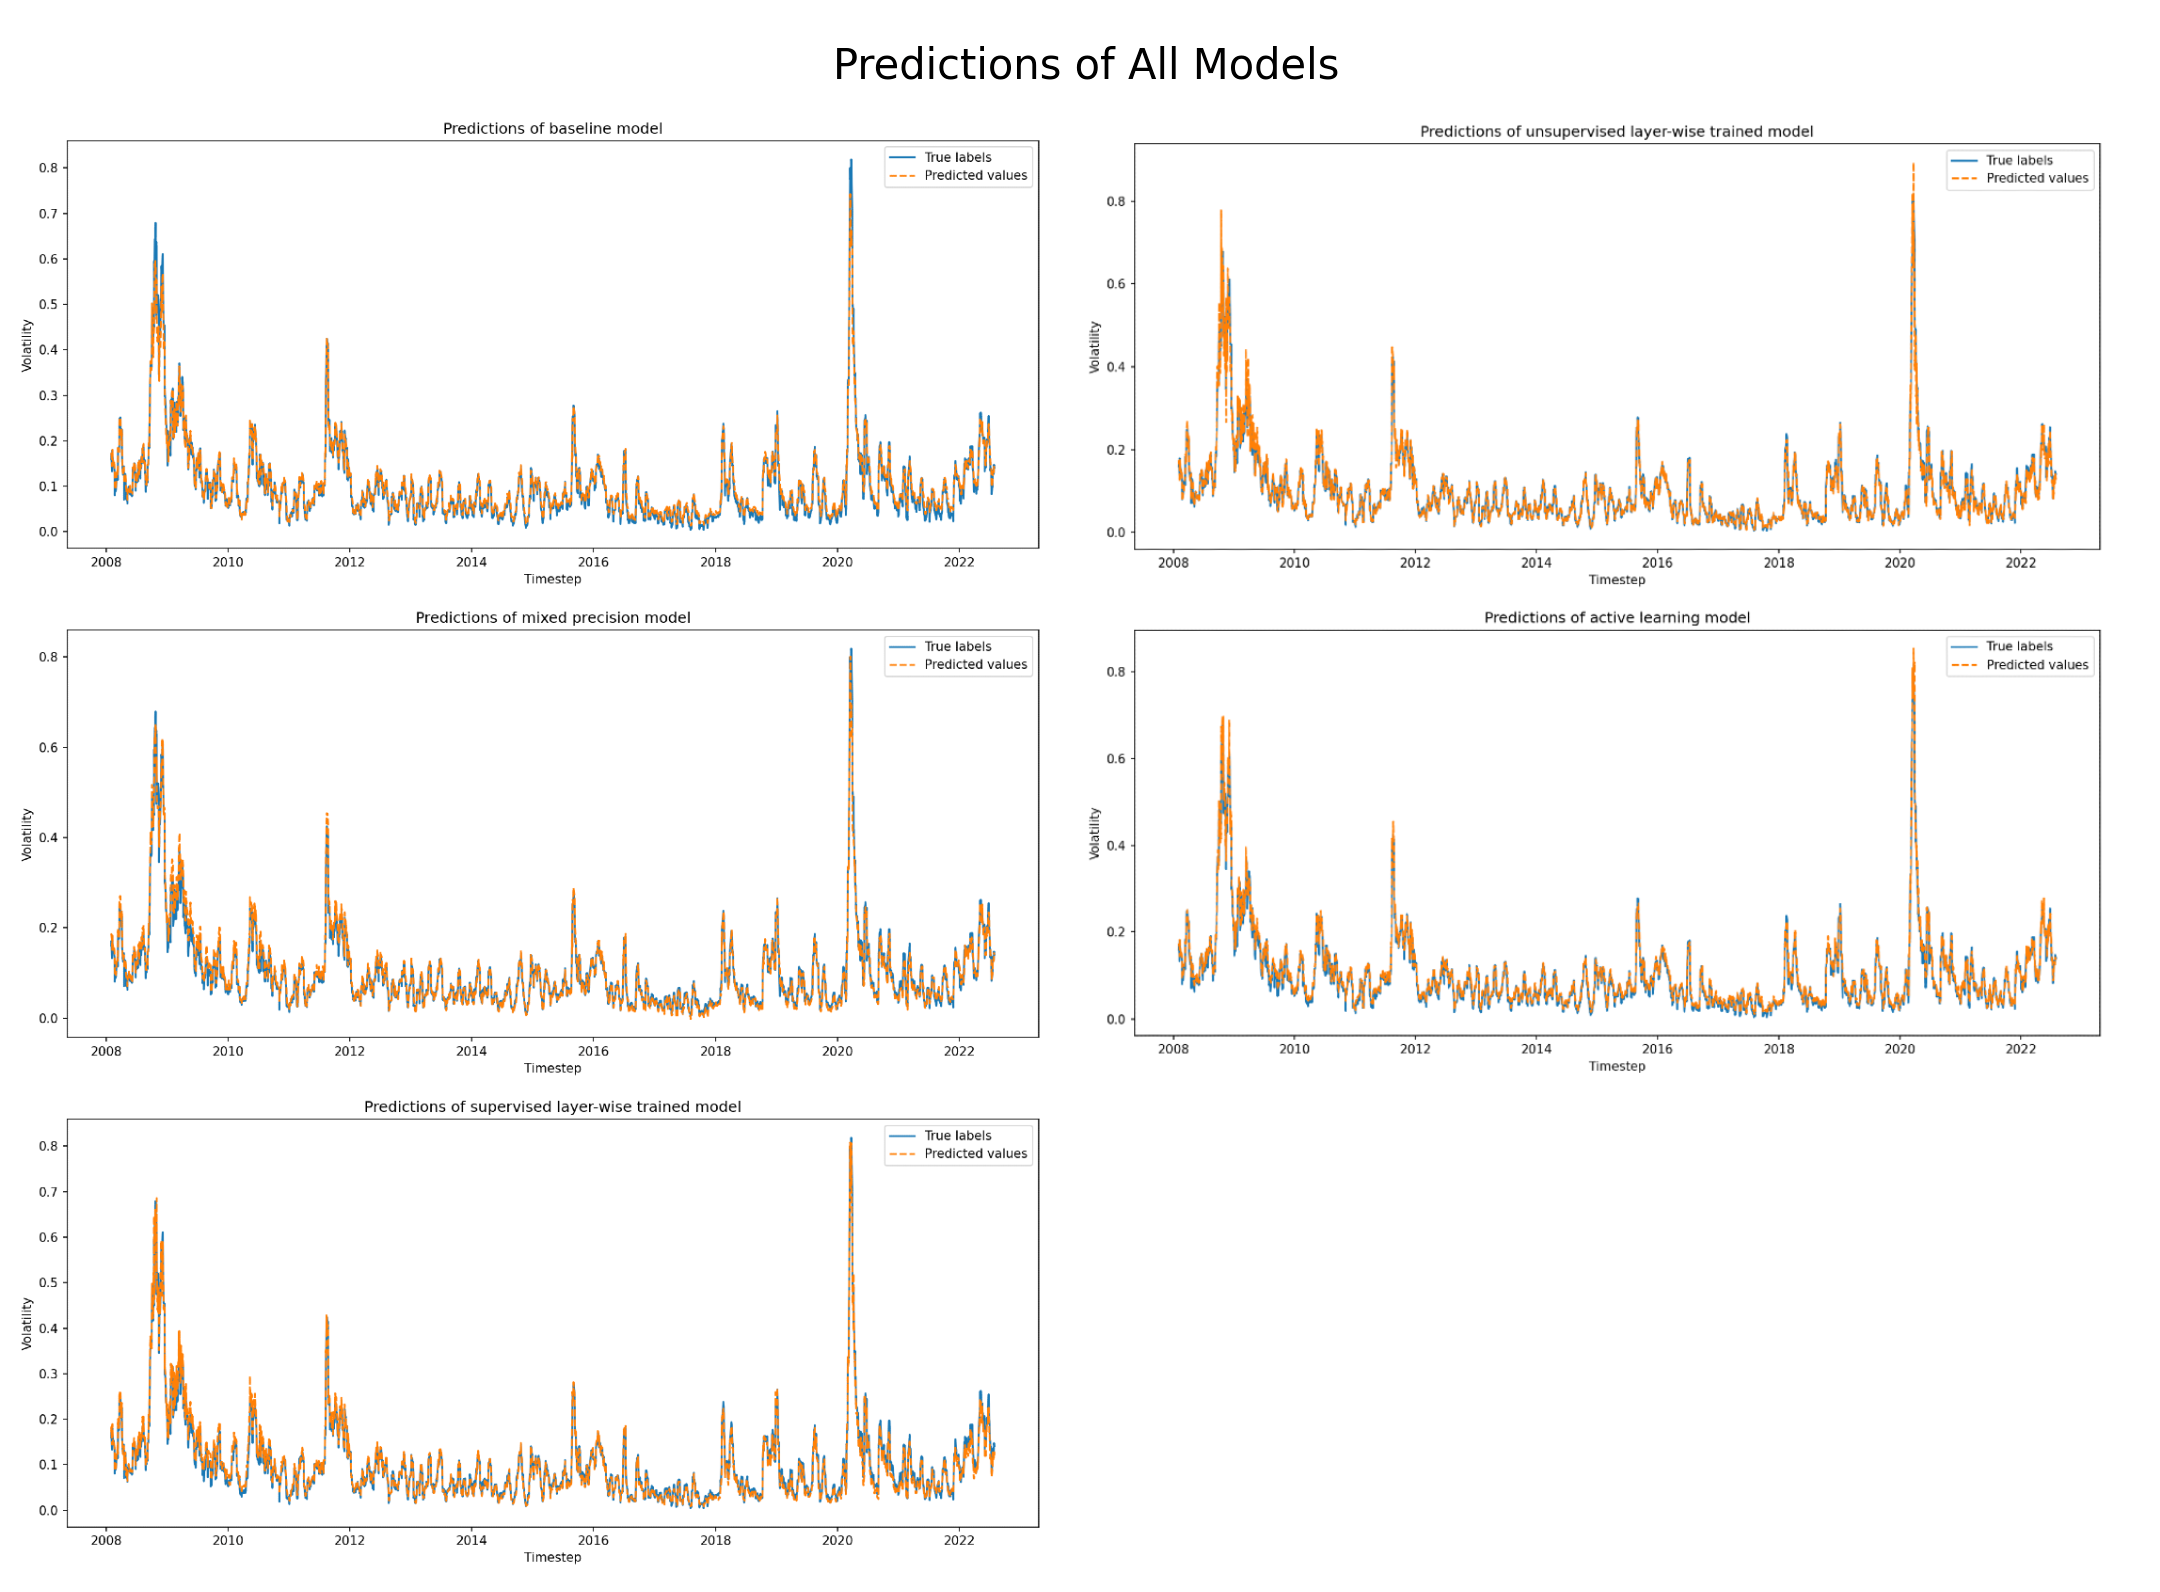
\includegraphics[width=\textwidth]{results/all-predictions.png}
        \caption{\centering Predicted volatility time series of each tested model (orange dashed line) against the true volatility time series (blue) over testing dataset.}
        \label{fig: predictions}
    \end{figure}


    Figure \ref{fig: predictions} demonstrates that all models  generate predictions that accurately follow the general trend of the true volatility sequence. However, close inspection of how the different models handle rapid volatility jumps highlights the differences in forecasting characteristics. If one inspects the significant rise in volatility in late 2008 (corresponding to the 2008 financial crisis), the baseline model is shown to underpredict the true volatility, undercutting the true peak by a fairly significant margin ($\hat{v}_{t+1} \approx 0.6$ when the true $v_{t+1}$ is closer to $0.7$). A similar characteristic can be seen in early 2020 (corresponding to the COVID19 pandemic) and soon thereafter, where the significant fluctuations in volatility are consistently underestimated by the DNN's predictions. This suggests that whilst the baseline DNN appears to model the smaller volatility changes very accurately, large, rapid changes in the true volatility result in less accurate predictions. 

    When the predicted time series of the other models are compared to that of the baseline, the differences in forecasting ability can be observed. Figure \ref{fig: predictions} shows that the models using supervised and unsupervised layer-wise pre-training most accurately represent both small and large fluctuations in volatility. These plots show the predictions $\hat{v}_{t+1}$ are significantly closer to the labels $v_{t+1}$ at times of high volatility (e.g. in 2008 and 2020). The forecast of the model trained through unsupervised layer-wise pre-training appears slightly less accurate than that of its supervised counterpart, as this model overestimates the volatility jumps in 2008 and 2020, however less extreme movements are modelled very accurately. The model developed through mixed-precision training also appears to generate predictions that lie closer to the true volatility than the baseline model, although with an accuracy slightly below that of the layer-wise pre-trained models.

    When considering the model trained through active learning, the forecast time series is also shown to accurately follow the path of the true volatility, with most fluctuations accurately captured. However, these predictions seem to slightly miss the true movements, as the scale of peaks and troughs seems to be consistently underestimated (underpredicting the value of $\hat{v}_{t+1}$ for peaks and overestimating it at troughs), suggesting this model is slightly less performant than other adapted approaches. However, the general trend of the predictions on a wider scale seems (at least) commensurate with those of the baseline model, indicating that the implemented active learning training process does not degrade forecasting performance.


    \section{Accuracy Results}

    To demonstrate the preformance of each trained model more precisely, Table \ref{table: accuracy} presents the results generated by evaluating the accuracy metrics presented in Section \ref{section: accuracy-metrics}. This began with the baseline model; it was found to exhibit an impressive test accuracy, demonstrating the great ability of the LSTM architecture to model sequences such as the utilised financial volatility time series. Namely, the coefficient of determination of the baseline model was found to be $0.977414$, showing that the sum of squared prediction errors between $\hat{v}_{t+1}$ and $v_{t+1}$ is close to zero (Equation \ref{eq: r-squared}). This means that the true labels have been near-perfectly represented by the model, demonstrating the DNN trained by a traditional training process can generate excellent one-step-ahead forecasts of the market volatility of the S\&P 500. Similarly, the baseline model produced impressive MAE and RMSE scores of $0.008407$ and $0.013830$, demonstrating that the average magnitude of the prediction error is near-zero. Importantly, both the MAE and RMSE are similar, indicating that the model is averse to uniformly distributed prediction errors (highlighted by the MAE) and highly deviant predictions (identified by the RMSE). The model also generated an impressive MAPE of $14.662217\%$, indicating that the DNN has fit the training data well.


    % accuracy metrics
    \begin{table}[ht]
        \centering
        \begin{tabular}{|l|l|l|l|l|} 
        \hline
        \textbf{Method}                                                               & $\mathbf{R^2}$ & \textbf{MAE} & \textbf{RMSE} & \textbf{MAPE (\%)}  \\ 
        \hline
        Baseline                                                                      & 0.977414       & 0.008407     & 0.013830      & 14.662217           \\ 
        \hline
        Mixed-precision                                                               & 0.977372       & 0.009121     & 0.013843      & 12.126700           \\ 
        \hline
        \begin{tabular}[c]{@{}l@{}}Supervised\\layer-wise pre-training\end{tabular}   & 0.985642       & 0.007814     & 0.011027      & 9.932409            \\ 
        \hline
        \begin{tabular}[c]{@{}l@{}}Unsupervised\\layer-wise pre-training\end{tabular} & 0.98406       & 0.00708     & 0.01162      & 8.80475           \\ 
        \hline
        Active Learning                                                               & 0.971119       & 0.010452     & 0.015639      & 11.08715           \\
        \hline
        \end{tabular}
        \caption{\centering Accuracy data for all methods, evaluated over the testing datset.}
        \label{table: accuracy}
    \end{table}


    After certifying the performance of the baseline model, the accuracy achieved by alternative training methods could be contextualised. This exploration began with an analysis of mixed-precision training; impressively, the mixed-precision model was had higher prediction accuracy than the baseline across almost all metrics, generating a $15.10\%$ lower MAE, $10.50\%$ lower MAPE, $8.53\%$ decrease in RMSE (Table \ref{table: accuracy}). These scores indicate that this training algorithm was capable of optimising a model that can forecast volatility more accurately than the baseline approach.

    Following this result, the two models using progressive training were analysed. The first model, trained through supervised layer-wise pre-training, exhibited higher forecasting accuracy than both the baseline and mixed-precision models that used traditional training algorithms. The optimised model produced an outstanding $R^2$ score of $0.985642$, indicating that using supervised layer-wise pre-training facilitated an almost perfect correspondence between $\hat{v}_{t+1}$ and $v_{t+1}$; additionally, this model reduced the MAPE of the baseline model by $32.26\%$ and the mixed-precision model by $18.09\%$. The accuracy improvement was observed across the board, generating better $R^2$, MAE, RMSE, and MAPE scores than both the baseline and mixed-precision methods. The model trained through unsupervised layer-wise pre-training also exhibited impressive performance, generating predictions of similar accuracy to its supervised counterpart, and significantly outperforming the baseline with $0.6800\%$ higher $R^2$, $15.78\%$ lower MAE, $15.98\%$ lower RMSE, and an exceptional decrease in MAPE of $39.95\%$. When directly comparing the models trained through supervised and unsupervised layer-wise pre-training, however, the differences are not so explicit. The supervised approach produced marginally better performance across the $R^2$ and RMSE metrics: the resultant model exhibited a $0.1607\%$ higher $R^2$ and $5.103\%$ lower RMSE. On the contrary, the unsupervised approach produced a model with a $9.393\%$ smaller MAE and $11.35\%$ smaller MAPE. This suggests that both supervised and unsupervised layer-wise pre-training produced a more accurate model than the baseline training algorithm, but each reduced prediction error differently: for example, the lower RMSE of the supervised pre-trained DNN indicates this model less frequently generates predictions that are highly incompatible with the true value. Thus, the accuracy results in Table \ref{table: accuracy} show that both supervised and unsupervised layer-wise pre-training are the most effective training methods for developing high-performance DNNs for volatility forecasting. 

    The active learning algorithm produced a model impressive MAPE, exhibiting a $24.38\%$ lower test MAPE than the baseline model. However, when considering other accuracy metrics, the model was not shown to exhibit such an accuracy benefit, having a slightly worse coefficient of determination ($0.6440\%$ lower) and noticeably increased test MAE ($24.33\%$ higher) and RMSE ($13.08\%$ higher). Thus, the performance of the active learning-based model was roughly equivalent to the baseline, outperforming it on some metrics but underperforming on others. When different parameterisations of the active learning training algorithm were explored, a few implementations did produce higher accuracy than the baseline; for example, when using 200 training iterations and a sample size of 70, a $26.83\%$ lower RMSE and $34.72\%$ lower MAPE were facilitated (but using $96.36\%$ of the full training dataset). Hence, these results indicate that active learning can be used to develop a model with similar performance to a traditionally trained baseline, supporting the assertion that this method can be tuned to only inflict a marginal accuracy detriment.


    \section{Efficiency Results}

    \subsection{Training Time Analysis}

    As outlined in Section \ref{section: efficiency-metrics}, total training time is one of the most applicable metrics for quantifying the energy efficiency of DL training algorithms in this context; hence, to examine the success of each training algorithm the time (in seconds) taken to optimise the DNN's parameters was quantified by profiling each implementation, the results of which are exhibited in Table \ref{table: efficiency}. This analysis found that the baseline training approach took a total of $198.602$ seconds to optimise the DNN; this result was then used to contextualise the efficiency of each subsequent training method. Firstly, mixed-precision training was examined, which produced a fairly disappointing result: the algorithm took $18.98\%$ longer to complete than in the baseline, despite using the same number of epochs. This suggests that utilising 16-bit floating-point representations for evaluating operations during training did not directly improve the energy efficiency of training the DNN.

    % efficiency metrics
    \begin{table}[ht]
        \centering
        \begin{tabular}{|l|l|} 
        \hline
        \textbf{Method}                                                               & \begin{tabular}[c]{@{}l@{}}\textbf{Total Training }\\\textbf{Time (s)}\end{tabular}  \\ 
        \hline
        Baseline                                                                      & 198.602                                                                              \\ 
        \hline
        Mixed-precision                                                               & 236.306                                                                              \\ 
        \hline
        \begin{tabular}[c]{@{}l@{}}Supervised \\layer-wise pre-training\end{tabular}  & 154.952                                                                             \\ 
        \hline
        \begin{tabular}[c]{@{}l@{}}Unsupervised\\layer-wise~pre-training\end{tabular} & 130.292                                                                             \\ 
        \hline
        Active learning                                                               & 212.453                                                                              \\
        \hline
        \end{tabular}
        \caption{\centering Total training time required for each implemented training process to produce a model with the accuracy outlined in the preceding accuracy table.}
        \label{table: efficiency}
    \end{table}


    On the contrary, both progressive training algorithms were shown to have significantly smaller training times, with unsupervised layer-wise pre-training being the fastest to complete. The unsupervised method facilitated a $34.40\%$ decrease in training time, whilst the supervised method improved on the baseline by $22.43\%$, but took $18.24\%$ longer than its unsupervised counterpart. These results indicate that unsupervised layer-wise pre-training is the most efficient way to train DNNs, taking the least amount of time to produce an accurate model, and hence likely being the most energy-efficient approach. Furthermore, it demonstrates that supervised unsupervised layer-wise pre-training are both viable ways to improve the energy efficiency of DNN training, as they both took significantly less time to train an accurate forecasting model than the baseline algorithm.

    When the training time of active learning is analysed, the results do not indicate that this is an effective method for reducing the overall length of training. Namely, the active learning algorithm using hyperparameters detailed in Section \ref{section: al-model} marginally exceeded the total time spent training by the baseline approach by $6.974\%$. This suggests that active learning is not an effective method for directly minimising the length of training. Although, a small proportion of the active learning parameterisations tested did result in a reduction in training time over the baseline algorithm, majoritively achieved by drastically limiting the number of training iterations and training dataset size, and hence in general also inflicted an accuracy drop (Table \ref{table: al-efficiency}). Despite this result, it is not concerning that total training time was not reduced, as active learning majoritively focuses on improving the data efficiency of training, not explicitly the energy efficiency. This process instead intends to improve the ESG impacts of DL by reducing resource requirements, data storage and labelling costs, and the energy consumption of large data centres.


    \subsection{Convergence over Training}

    To further quantify the efficiency of each training approach, the convergence of the training error towards the minimum of the loss function was evaluated (Figure \ref{fig: convergence}). The plots show the prediction error output by the loss function on input of the training dataset and on input of a smaller validation set (a collection of data instances held back from the training process) at each epoch.


    \begin{figure}[ht!]
        \centering
        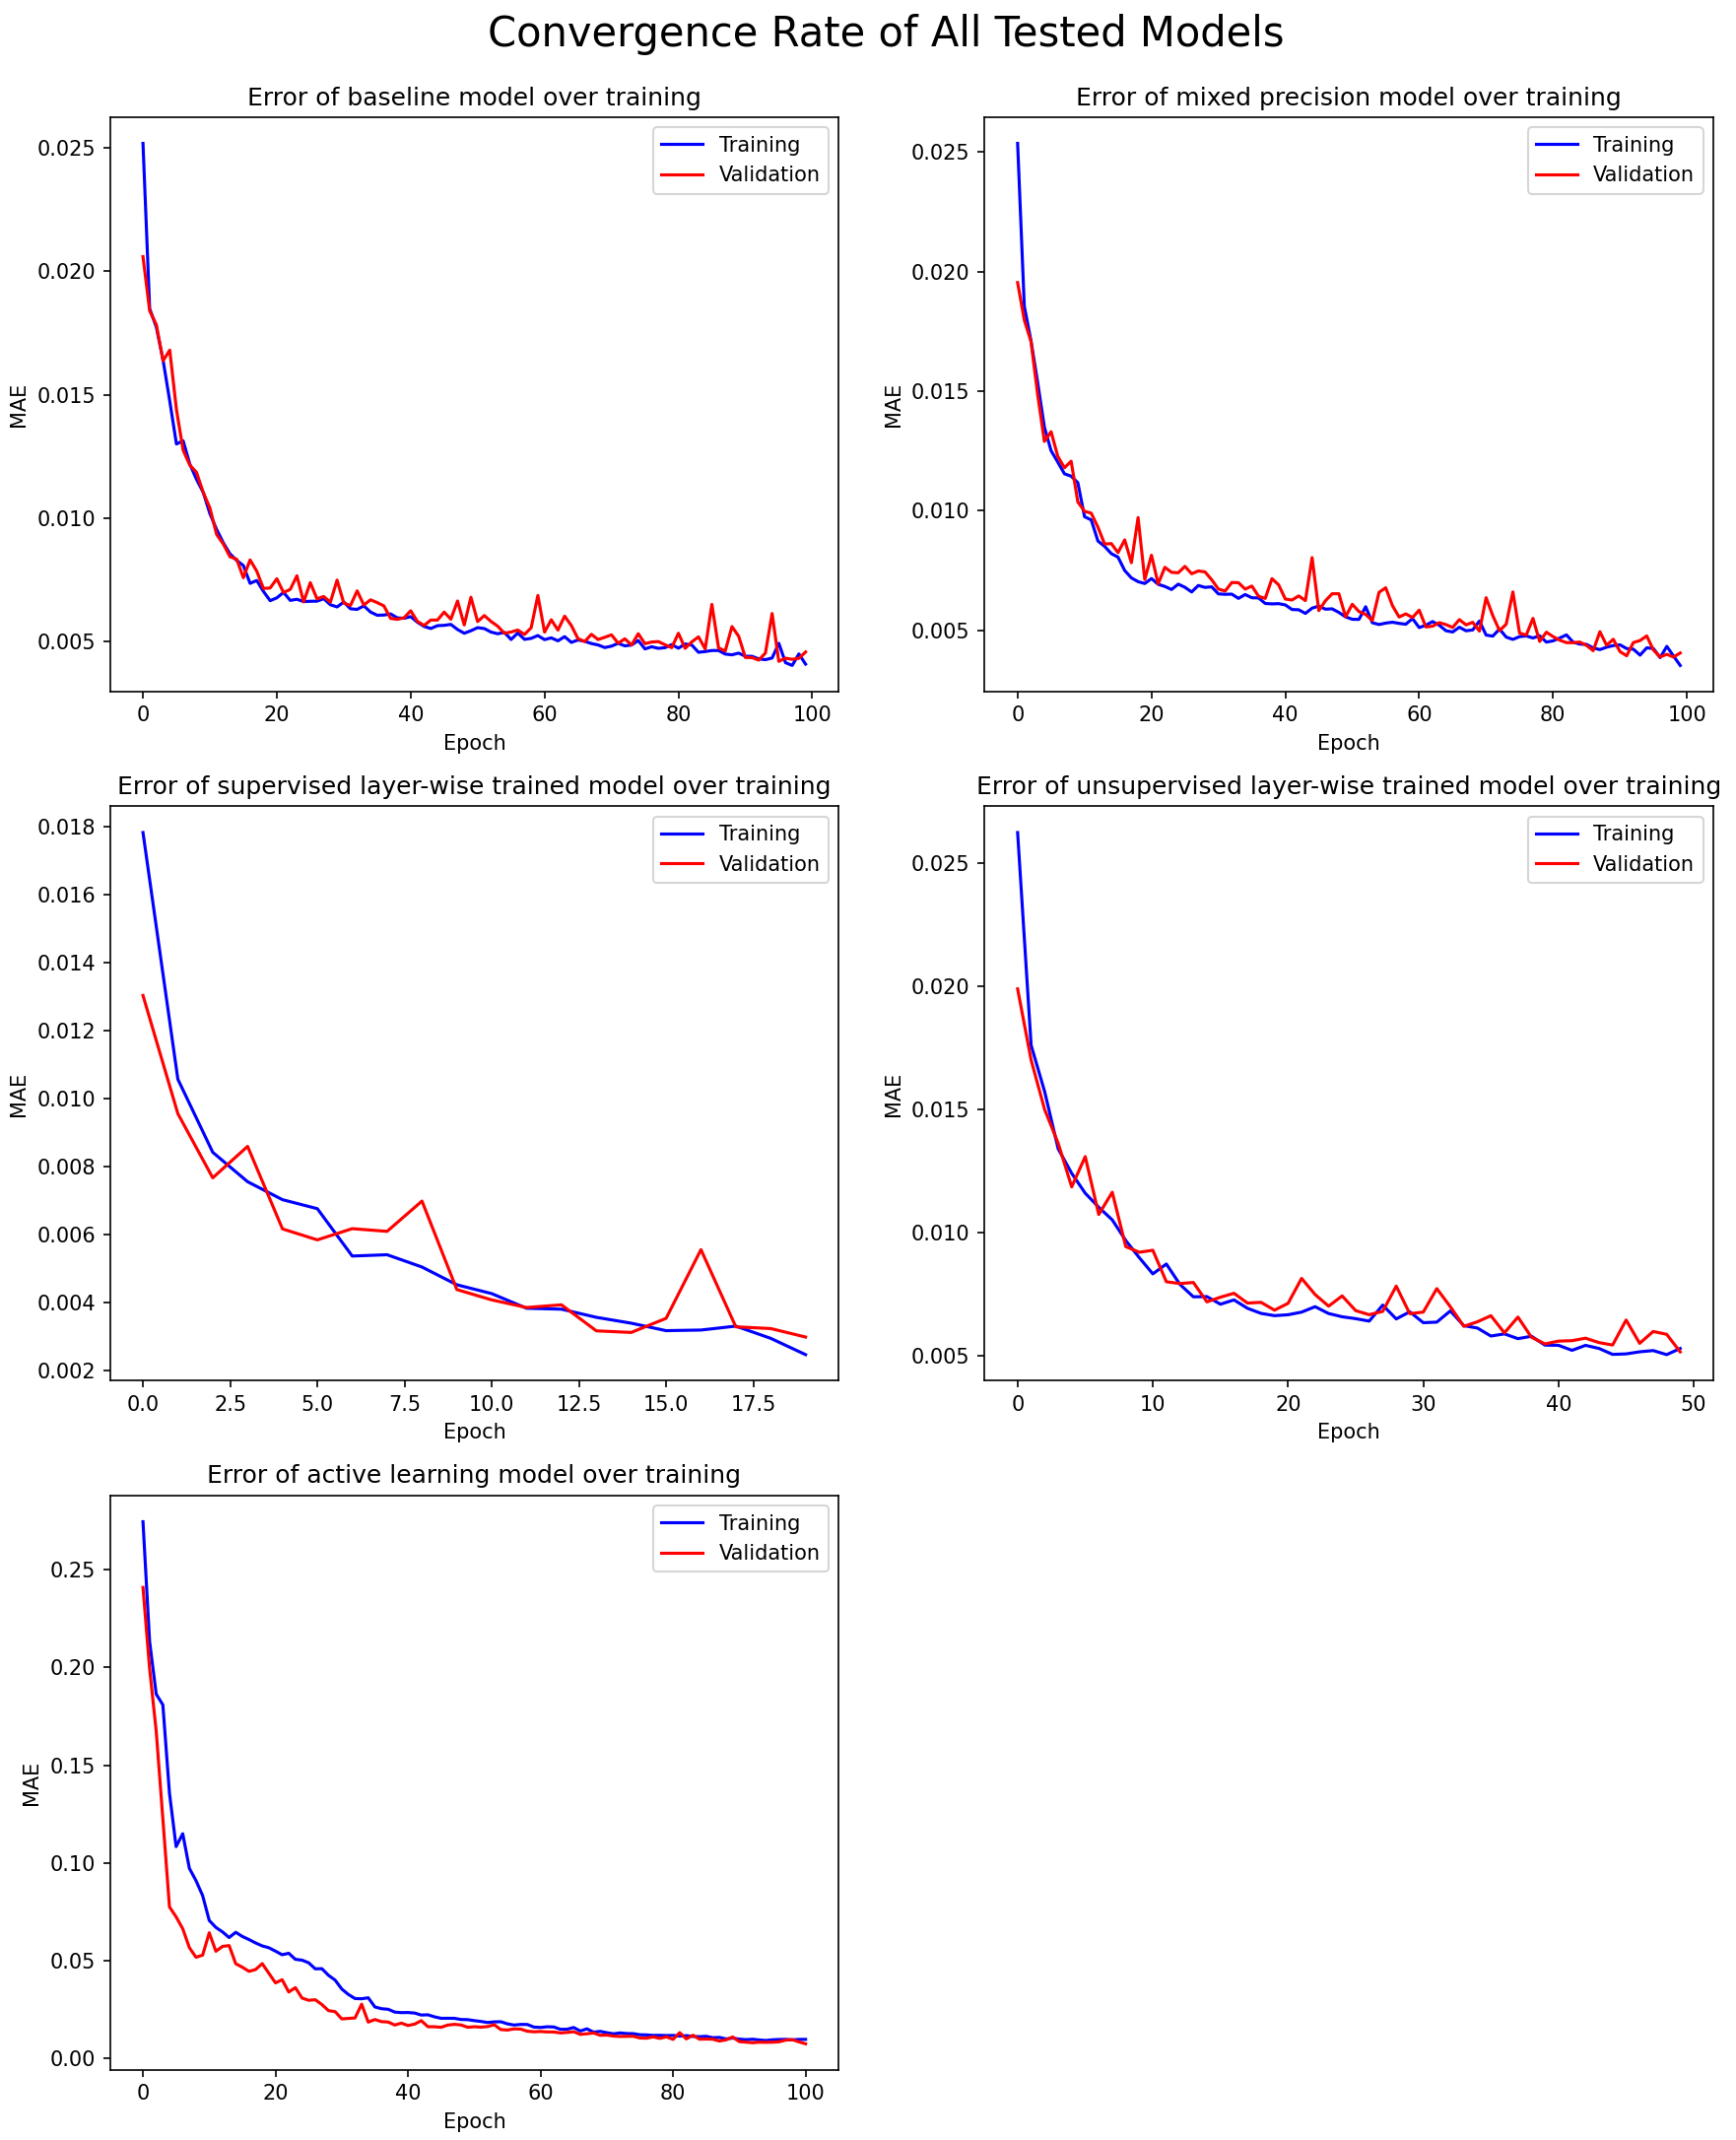
\includegraphics[width=\textwidth]{results/all-training-loss.png}
        \caption{\centering Convergence over each tested DNN training algorithm, shown as the progression of the output of the loss function (MAE) used at each epoch to determine the prediction error of the networkn (with a steeper gradient indicating a faster convergence rate).}
        \label{fig: convergence}
    \end{figure}

    When the convergence of the mixed-precision training process is compared to the baseline algorithm, a very similar trend can be seen; both exhibit closely aligned training and validation error curves, implying the models fit well to the training data, and both exhibit a significant decrease in MAE at the start of training with this tapering off in later epochs. The close similarities between both plots suggest that whilst introducing mixed-precision representations has not sped up the training process in terms of convergence per epoch, using these lower bit representations has not degraded the convergence rate of the prediction error towards the minimum of the loss function. Although, upon close inspection of the progression of the validation error over the mixed-precision training process, the curve appears to be slightly rougher than in the baseline case, exhibiting marginally larger fluctuations around the general trend line of convergence over the training process. This suggests that the mixed-precision training algorithm may be slightly less stable than when using high-precision representations.

    Comparison of the convergence of the two progressive training algorithms demonstrates the differences between these algorithms. Firstly, one can see that the pre-trained DNNs require significantly fewer epochs to optimise the full parameter set than the other training algorithms: the supervised and unsupervised methods only requiring $20$ and $50$ epochs respectively over the full network. Additionally, the initial epochs of both of these algorithms are shown to exhibit a much faster convergence, reducing both the training and validation error much more rapidly. Furthermore, the majority of their minimisation of prediction error within the first 10 epochs, whereas the same reduction is spread over the first 20 epochs in the baseline training process. For example, of the total reduction of validation error from $\sim \! 0.013$ to $\sim \! 0.003$ produced by the supervised approach, $90\%$ occurs within the first 10 epochs (decreasing the MAE to $\sim \! 0.004$). Similarly, $80\%$ of the total reduction in validation MAE ($\sim \! 0.02 \to \; \sim \! 0.005$) in the unsupervised case happens over the first 11 epochs of full network training ($\sim \! 0.02 \to \; \sim \! 0.008$). This indicates that progressive training is a significantly more efficient training approach as it induces faster learning within the DNN.

    Analysis of the convergence over active learning similarly highlights its ability to induce faster learning within a DNN than the baseline algorithm. This is indicated through the incredibly sharp decline in both training and validation error over the early stages of training, generating approximately $83\%$ of the total reduction in validation MAE over the first $8$ epochs. Furthermore, whilst in the baseline case the convergence rate slows considerably after the initial decline in MAE, significantly plateauing after the first $20$ epochs, during active learning the convergence rate stays higher for longer. Namely, a significant reduction in MAE is still observed up to approximately the 32nd epoch. This suggests that the learning process is more efficient as the network's parameters are optimised more rapidly in the early stages of training.


    \subsection{Efficiency Breakdown of Progressive Training}

    To further analyse the benefit provided by progressive training, a detailed study was conducted into the time taken by the supervised and unsupervised layer-wise pre-training algorithms, breaking down how these approaches improve training efficiency (Table \ref{table: progressive-efficiency}). These results demonstrate the different approaches taken by the progressive training algorithms, laying out how much time (and how many epochs) was spent on pre-training and tuning. 
    
    % progressive learning efficiency
    \begin{table}[ht]
        \centering
        \begin{tabular}{|l|l|l|l|l|l|l|l|l|} 
        \hline
        \begin{tabular}[c]{@{}l@{}}\textbf{\footnotesize Pre-Training}\\\textbf{\footnotesize Method}\end{tabular} & \begin{tabular}[c]{@{}l@{}}\textbf{\footnotesize Pre-}\\\textbf{\footnotesize Training}\\\textbf{\footnotesize Time~(s)}\end{tabular} & \begin{tabular}[c]{@{}l@{}}\textbf{\textbf{\footnotesize Pre-}}\\\textbf{\footnotesize Training}\\\textbf{\footnotesize Epochs}\end{tabular} & \begin{tabular}[c]{@{}l@{}}\textbf{\footnotesize Layer}\\\textbf{\footnotesize 1~(\%)}\end{tabular} & \begin{tabular}[c]{@{}l@{}}\textbf{\footnotesize Layer}\\\textbf{\footnotesize 2~(\%)}\end{tabular} & \begin{tabular}[c]{@{}l@{}}\textbf{\footnotesize Layer}\\\textbf{\footnotesize 3~(\%)}\end{tabular} & \begin{tabular}[c]{@{}l@{}}\textbf{\footnotesize Tuning}\\\textbf{\footnotesize Time}\\\textbf{\footnotesize (s)}\end{tabular} & \begin{tabular}[c]{@{}l@{}}\textbf{\footnotesize Tuning}\\\textbf{\footnotesize Epochs}\end{tabular} & \begin{tabular}[c]{@{}l@{}}\textbf{\footnotesize Total}\\\textbf{\footnotesize Time}\\\textbf{\footnotesize (s)}\end{tabular}  \\ 
        \hline
        None                                                                             & -                                                                                             & -                                                                                                                    & -                                                                         & -                                                                        & -                                                                        & 198.60                                                                                  & 100                                                                      & 198.60                                                                                  \\ 
        \hline
        Supervised                                                                       & 107.89                                                                                        & 20                                                                                                                   & 32.6                                                                      & 29.0                                                                     & 38.4                                                                     & 47.066                                                                                  & 20                                                                       & 154.95                                                                                  \\ 
        \hline
        Unsupervised                                                                     & 43.769                                                                                        & 7                                                                                                                    & 27.4                                                                      & 47.8~                                                                    & 24.7                                                                     & 86.523                                                                                  & 50                                                                       & 130.29                                                                                  \\
        \hline
        \end{tabular}
        \caption{\centering The time taken by pre-training and full network tuning for both supervised and unsupervised layer-wise pre-training (including a breakdown of the time spent pre-training each of the 3 internal LSTM layers), compared to the total time taken by the baseline method.}
        \label{table: progressive-efficiency}
    \end{table}


    This study found that supervised layer-wise pre-training was most effective when 20 epochs were used to pre-train each layer, with another 20 epochs used to optimise the full network; in comparison, the unsupervised approach generated the best performance when employing only 7 epochs per pre-training round, then a final tuning round of 50 epochs. Thus, in total the supervised method used 60 low-cost epochs (training only a single layer) and 20 high-cost epochs, whereas the supervised method only employed 21 low-cost epochs but required 50 high-cost epochs. Table \ref{table: progressive-efficiency} illustrates this divergence by showing the proportion of the total training time spent pre-training; the supervised approach allocated $69.63\%$ to this stage, compared to only $33.59\%$ during the unsupervised algorithm. Therefore, whilst unsupervised layer-wise pre-training had a shorter total training time, supervised pre-training facilitated a greater reduction in the required number of full DNN tuning epochs to exceed the performance of the baseline method (exhibiting an $80\%$ decrease in tuning epochs, compared to a $50\%$ decreasing when using the unsupervised approach).

    Table \ref{table: progressive-efficiency} also breaks down how each pre-training round contributed to the overall computational cost of training. Of the total pre-training time, the supervised method spent $32.6\%$ on the first layer of the network, $29.0\%$ on the second, and $38.4\%$ on the final layer. Hence, the second hidden layer was faster to pre-train than the initial base model (suggesting the transfer of knowledge between these rounds), but the final layer was the most computational intensive of all (possibly due to deep layers containing higher-dimensional representations). A different trend was seen over unsupervised pre-training, where the second hidden layer was the most computationally intensive (using $32.6\%$ of the pre-training time), and the final layer was the fastest ($24.7\%$ of pre-training); this is likely due to the 2nd layer building up the majority of the encoding (of the input vector) within the autoencoder, meaning the 3rd hidden layer was not required to add as much to the representation learning process (simply building upon the knowledge of its preceding autoencoder layer).


    \subsection{Data Efficiency of Active Learning}

    Once the energy efficiency of the baseline, mixed-precision, and progressive training algorithms had been thoroughly explored, the data efficiency of active learning was examined. Since this approach focusses on simultaneously minimising both the training dataset size and the accuracy drop inflicted by this constriction, active learning can implement a spectrum of accuracy-efficiency compomises. To explore these varying compromises, different parameterisations of active learning algorithms were experimented with, manipulating the hyperparameters controlling the number of training iterations and sample size $n_{sample}$. 

    \begin{table}[ht]
        \centering
        \begin{tabular}{|l|l|l|l|l|l|l|l|} 
        \hline
        \textbf{\footnotesize Method}                                                            & \begin{tabular}[c]{@{}l@{}}\textbf{\footnotesize Number of}\\\textbf{\footnotesize Iterations}\end{tabular} & \begin{tabular}[c]{@{}l@{}}\textbf{\footnotesize Sample}\\\textbf{\footnotesize Size}\end{tabular} & \begin{tabular}[c]{@{}l@{}}\textbf{\footnotesize Final Pool}\\\textbf{\footnotesize Size}\end{tabular} & \begin{tabular}[c]{@{}l@{}}\textbf{\footnotesize Utilisation of}\\\textbf{\footnotesize Full Training}\\\textbf{\footnotesize Dataset (\%)}\end{tabular} & \textbf{\footnotesize RMSE}    & \textbf{\footnotesize MAPE}     & \begin{tabular}[c]{@{}l@{}}\textbf{\footnotesize Training}\\\textbf{\footnotesize Time (s)}\end{tabular}  \\ 
        \hline
        Baseline                                                                   & -                                                                               & -                                                                      & 14600                                                                      & 100                                                                                              & 0.013830         & 14.662217         & 198.602                                                                       \\ 
        \hline
        \multirow{12}{*}{\begin{tabular}[c]{@{}l@{}}Active\\Learning\end{tabular}} & \multirow{3}{*}{\textit{200 }}                                                  & 70                                                                     & 14070                                                                      & 96.36                                                                                            & 0.01012          & 9.57100          & 480.603                                                                       \\ 
        \cline{3-8}
                                                                                &                                                                                 & 45                                                                     & 9045                                                                       & 61.95                                                                                            & 0.01492          & 10.47995          & 436.716                                                                       \\ 
        \cline{3-8}
                                                                                &                                                                                 & \textit{20}                                                            & \textit{4020}                                                              & \textit{27.53}                                                                                   & \textit{0.01863} & \textit{14.03773} & \textit{222.579}                                                              \\ 
        \cline{2-8}
                                                                                & \multirow{3}{*}{150}                                                            & 90                                                                     & 13590                                                                      & 93.08                                                                                            & 0.01404          & 12.25406          & 363.479                                                                       \\ 
        \cline{3-8}
                                                                                &                                                                                 & 55                                                                     & 8305                                                                       & 56.88                                                                                            & 0.01595          & 13.57484          & 326.668                                                                       \\ 
        \cline{3-8}
                                                                                &                                                                                 & 20                                                                     & 3020                                                                       & 20.68                                                                                            & 0.02579          & 25.93023          & 274.484                                                                       \\ 
        \cline{2-8}
                                                                                & \multirow{3}{*}{\textit{100 }}                                                  & 140                                                                    & 14140                                                                      & 96.85                                                                                            & 0.01740          & 15.03445          & 239.561                                                                       \\ 
        \cline{3-8}
                                                                                &                                                                                 & \textit{80}                                                            & \textit{8080}                                                              & \textit{55.34}                                                                                   & \textit{0.015639} & \textit{11.08715} & \textit{212.453}                                                              \\ 
        \cline{3-8}
                                                                                &                                                                                 & 20                                                                     & 2020                                                                       & 13.84                                                                                            & 0.03527          & 29.82608          & 175.556                                                                       \\ 
        \cline{2-8}
                                                                                & \multirow{3}{*}{50}                                                             & 250                                                                    & 12750                                                                      & 87.33                                                                                            & 0.01735          & 13.69113          & 176.087                                                                       \\ 
        \cline{3-8}
                                                                                &                                                                                 & 135                                                                    & 6885                                                                       & 47.16                                                                                            & 0.02580          & 22.39938          & 124.031                                                                       \\ 
        \cline{3-8}
                                                                                &                                                                                 & 20                                                                     & 1020                                                                       & 6.99                                                                                             & 0.03883          & 41.60770          & 89.6995                                                                       \\
        \hline
        \end{tabular}
        \caption{\centering Results of the experimentation into how varying the number of training iterations and sample size effect the data efficiency, resulting accuracy, and training time of an active learning based training algorithm (using GSx and GSy). N.B. notable results are emphasised in italics.}
        \label{table: al-efficiency}
    \end{table}


    Table \ref{table: al-efficiency} outlines the results of this study, enumerating the different hyperparameters used and the resulting data efficiency, accuracy, and training time achieved. The results demonstrate the general trend that the greater the number of active learning iterations, and the more data added at each iteration, the higher the achieved model accuracy but the lower the data and time efficiency of training. For example, the hyperparameters $(N_{iters}, n_{sample}) = (200, 70)$ facilitated a highly performant DNN with a test MAPE of $9.57100$ (a $34.72\%$ decrease from the baseline model), but this required using most of the training data ($96.36\%$ of the full dataset) and a considerably longer training time ($142.0\%$ increase over the baseline).

    However, by tuning these hyperparameters the ability of active learning to facilitate accurate performance whilst considerably reducing training data requirements was shown. Under the hyperparameters $(N_{iters}, n_{sample}) = (200, 20)$, this approach surpassed the performance of the baseline model (reducing the test MAPE by $4.259\%$) using only $27.53\%$ of the amount of training data. Furthermore, whilst this did inflict a longer training time than the baseline, an increase of only $12.07\%$ was observed, suggesting the direct computational cost was not significantly inflated. Another notable parameterisation $(N_{iters}, n_{sample}) = (100, 80)$ was able to produce a model with significantly improved MAPE ($24.38\%$ lower than the baseline) using only $55.34\%$ of the training data, and only inflicting a $6.974\%$ increase in training time. The impressive result solidified this parameterisation as the implementation used to compare the performance of active learning to the other implemented training algorithms in the preceding section.


    \subsection{Summary}

    Hence, mixed-precision training and both progressive training algorithms were shown to provide an accuracy benefit over the baseline model, with unsupervised layer-wise pre-training facilitating the greatest performance improvement. Additionally, active learning was shown to produce performance at least commensurate to that of the baseline. When considering the efficiency of each model, the mixed-precision algorithm generated dissapointing results, exhibiting similar convergence but a longer training time. However, both progressive training methods were able to significantly reduce training time, whilst active learning was able to considerably restrict the training dataset without impacting performance; additionally, both progressive training and active learning achieved greater convergence rates, showing these algorithms learn more intelligently than the baseline approach.


    \section{Extended Discussion}

    Given the presented results outlining the accuracy and efficiency of each training algorithm, an evaluation can be made surrounding how well each reduces the computational cost and resource requirements of training, demonstrating their utility for lowering the ESG costs of Fintech.


    \subsection{Mixed-Precision Training}

    The implemented mixed-precision training approach attempts to reduce the computational cost of developing DNNs by lowering the precision at which operations within a DNN are evaluated. The experimentation found that whilst mixed-precision training did result in a higher accuracy model than the baseline, the training process took $18.98\%$ longer, suggesting this approach did not directly improve energy efficiency. However, a nearly identical convergence rate towards the minimum of the loss function over this training process was demonstrated, suggesting that reducing the memory requirements of DNN training by using smaller $16$-bit representations does not negatively impact the stability of training and performance of the resulting model.

    Since the mixed-precision implementation was not shown to facilitate a reduction in training time, there is no evidence found in this research to suggest that mixed-precision representations are an effective method for improving the energy efficiency of training DNNs for financial volatility forecasting. This is a disappointing conclusion, as it does not echo the results of reduced precision implementations in other fields that have boosted training speed, such as DoReFa-Net \citep{zhou-2016} which showed the benefit of low-bit training to CNN-based image classifiers. However, this is not that surprising, as DoReFa-Net inflicted a significant reduction in precision (using 1-bit parameters, 2-bit activations, and 6-bit gradients) which was not undertaken in this research; instead, $16$-bit representations were used, which cannot be expected to facilitate the same efficiency improvement as that of \citet{zhou-2016}. Furthermore, the presented findings more closely resemble those of \citet{ott-2017}, who found that low-bit training was not ubiquitously effective for improving the efficiency of training RNNs; hence, the results presented in this thesis may suggest that LSTM-based volatility forecasting may be one such application.

    The lack of efficiency benefit may also be explained by the model architecture and hardware utilised. Namely, the implemented DNN (and training dataset) is relatively small compared to state-of-the-art implementations developed in cutting-edge DL research and the expensive systems typically used by large institutions. Due to the overhead costs within model training, smaller models do not typically benefit from mixed-precision to the same extent as those with more complex architectures, as these overheads constitute a large portion of the training time. Furthermore, hardware accelerators (such as the GPUs relied upon in this study) do not provide as much benefit to smaller models, as the matrix multiplications are not as computationally intensive and so do not benefit as much from increased parallelisation. Therefore, whilst no training time reduction was witnessed in this research, this method may still hold promise in improving the energy efficiency of the higher complexity systems used by financial institutions. 

    Hence, this research did not uncover any benefit of mixed-precision training in improving the energy efficiency of DL in finance and thus did not confirm the research hypothesis. However, one limitation of this research is that the memory consumption over DNN training was not explored; thus, this research does not quantify any reductions to memory usage that may have been facilitated by mixed-precision representations, which could have revealed other efficiency improvements.


    \subsection{Progressive Training}

    On the contrary, both progressive training approaches were able to significantly reduce total training time whilst producing a DNN with higher prediction accuracy. Supervised layer-wise pre-training improved the MAPE of the baseline model by $32.26\%$, whereas the unsupervised approach generated a $\sim \! 15\%$ decrease in MAE and RMSE and an impressive $39.95\%$ reduction in MAPE. These results indicate that the true volatility time series has been accurately represented by the predictions of the trained model, enabling accurate predictions. Furthermore, a high convergence rate is exhibited over both progressive training approaches, demonstrating the stability and robustness of the training algorithms. The significant reduction to training time in both cases ($22.43\%$ and $34.40\%$ faster in the supervised and unsupervised cases respectively) also suggests that supervised and unsupervised layer-wise pre-training are successful at improving the energy efficiency of training DNNs in this context, as shorter training times likely correspond to lower energy consumption.

    These results align with other research into progressive training completed further afield, similarly highlighting the efficiency of progressive training algorithms. For instance, \citet{ienco-2019} found supervised layer-wise pre-training improved the generalisability of sequence classifiers, which is similarly shown in the high testing accuracy of the presented models. Additionally, \citet{xu-2018} and \citet{sagheer-2019} found unsupervised layer-wise pre-training could induce faster convergence whilst improving accuracy, both of which are demonstrated in the results of this research. Hence, this study supports the findings of other research into progressive training, extending the known utility of this Green AI method to the field of financial market volatility forecasting.

    Another core success shown by both algorithms was their ability to significantly reduce the number of epochs spent optimising the parameter set of the full network. The supervised approach reduced the required tuning rounds by $80\%$ to $20$ epochs and the supervised approach lowered it by $50\%$ to $50$ epochs. Since optimising the full 3-layer LSTM network is significantly more computationally intensive than optimising only a single LSTM layer (due to the higher number of parameters, calculations, and updates), this reduction in tuning likely facilitated a significant decrease in the computational cost of training. This was likely facilitated by the layer-wise pre-training stage inducing faster optimisation of the parameters, as the number of epochs in total over both the pre-training and tuning stages was still lower than in the baseline case. Thus, the low-cost pre-training epochs were shown to be effective at teaching the DNN how to make accurate predictions, allowing it to learn faster than possible in the traditional baseline algorithm. Furthermore, this efficiency benefit was likely facilitated by the transfer of useful information learned by each layer over pre-training to the subsequently added layer, allowing parameter updates to incorporate information already learned about the features of the input (as \citet{xu-2021} posited). This is shown through layers added later during pre-training (in general) making up a lower proportion of the total pre-training time. During supervised pre-training, $29.0\%$ of the total time was allocated to training the second LSTM layer, compared to $32.6\%$ spent on the first. Similarly, the unsupervised approach expended $27.4\%$ of pre-training on the first hidden layer and only $24.7\%$ on the last. Thus, these results demonstrate that supervised and unsupervised layer-wise pre-training facilitate a more intelligent and efficient learning process. 

    One limitation of layer-wise pre-training is the extra computational cost of fixing the parameters of previously pre-trained layers such that they aren't optimised in subsequent pre-training rounds. When profiling the progressive training algorithms, this cost was included in the pre-training time recorded per layer; thus, the total time calculated is not solely attributed to model training. This means there is a slight divergence between what is included in the total training time statistic between the progressive training algorithms and the baseline. Additionally, more time is spent on auxiliary tasks during each subsequent pre-training round than when training the initial base network, as the first round does not fix any parameters. This may contribute to why some hidden layers added during pre-training do not exhibit an increased training speed from the layer preceding it. However, these must be included in the total times attributed to progressive training to ensure a fair comparison to the baseline method which does not require these auxiliary tasks.

    An interesting difference between the supervised and unsupervised approaches is that the supervised method allocated $69.63\%$ of the total training time to pre-training, compared to only $33.59\%$ during the unsupervised algorithm (which spent more time tuning). This distinction is likely due to the supervised algorithm training the DNN to forecast volatility from the start, whereas the unsupervised approach pre-trained the DNN as an autoencoder. Time series forecasting is known to be a challenging task, but this is not so much the case with representation learning, as training an autoencoder to solely minimise the reconstruction error between inputs and outputs is significantly simpler than forecasting future values. Thus, more epochs were required to produce an accurate DNN over supervised pre-training than in the unsupervised case. However, later stages of unsupervised layer-wise pre-training required the developed autoencoder to be converted into a forecasting model, hence requiring more full network tuning epochs.

    The observed lower training times, fewer epochs, and computational cost savings indicate that both supervised and unsupervised layer-wise pre-training algorithms improve the energy efficiency of training a DNN for financial volatility forecasting. Whilst the observed reductions in training time have been on the scale of seconds in this research, when the model architecture and training length are scaled up to be comparable to the large, energy-intensive DL systems utilised in the upper echelons of computational finance research and by large financial institutions, these savings will likely also scale, allowing more significant reductions in training time (in the scale of hours and days) and carbon emissions. This adequately fills the research gap by proving that progressive training is an effective Green AI method for improving the energy efficiency of DL in finance, thus proving a possible route through which the carbon emissions of Fintech can be reduced, aligning Fintech more closely with the SDGs of sustainable finance. Moreover, this research has additionally improved the inclusivity of DL for finance, as shorter training times and smaller energetic costs lower the resource requirements of developing DNNs, reducing the expense of implementing such a system, and hence allowing more financial players and researchers to reap the benefits of DL.


    \subsection{Active Learning}

    As discussed by \citet{bender-2021} and \citet{walsh-2021}, a significant portion of the computational cost of high-performance DNNs can be attributed to their inefficient use of data. Thus, to further mitigate the ESG impacts of Fintech this research explores a data-efficient training algorithm known as active learning; this approach selects data instances more intelligently, reducing the training dataset size and minimising memory and energy costs.

    The completed study demonstrated the spectrum of efficiency-accuracy compromises achievable by active learning, ranging from the parameterisation $(N_{iters}, n_{sample}) = (200, 20)$ which maintained a comparable test MAPE to the baseline model using only $27.53\%$ of the data, to the parameterisation $(100, 80)$ which facilitated a $24.38\%$ improvement to MAPE using only $55.34\%$ of the training data (Table \ref{table: al-efficiency}). This shows that active learning is an effective approach for significantly reducing the amount of training data required to develop accurate DNNs in the chosen context; this lines up with the research of \citet{ren-2021}, who showcase the ability of active learning to deal with high-dimensional data in CV, and the results of \citet{peng-2017} and \citet{zimmer-2018} who both demonstrated benefits of active learning to reducing dataset sizes in other time series modelling domains. Hence, the presented research has built upon this preceding work to demonstrate that active learning is effective at improving the data efficiency of DNNs used in finance.

    By reducing the training data used within each epoch, it is likely active learning also reduced the total computational cost of training. One method of approximating the computational cost of each epoch is by estimating the number of parameter optimisation iterations (i.e. applications of gradient descent over the full parameter set) per epoch. If we have a training dataset of $N$ instances and utilise a batch size $b$, there will be a total of $\frac{N}{b}$ full parameter optimisation iterations at each epoch, as the DNN's parameter set is iteratively updated over the full training dataset one batch at a time. In the baseline case, there are $\frac{14600}{32} \approx 456.25$ parameter optimisation iterations per epoch. If this cost is to be computed for an active learning approach, the equivalent figure for training dataset size must be approximated as the average pool set size over the entirety of training. For the parameterisation $(N_{iters}, n_{sample}) = (100, 80)$ we begin with a seed pool of $80$ instances, and finish training with a pool set of size $8080$, meaning on average a pool of $N_{pool} = 4080$ instances was employed. Therefore, the active learning algorithm on average employs $\frac{4080}{32} \approx 127$ parameter optimisation iterations per epoch. Thus, the training dataset employed means the calculation of significantly fewer prediction errors and parameter updates, reducing the computational cost of each epoch and the full training process of optimising the network's parameter set.

    \citet{ren-2021} assert that this reduction in training data is facilitated through more intelligent data selection. The presented findings support this assertation, as the active learning algorithm exhibits a higher convergence rate, maintained over a greater number of epochs; hence, this approach more rapidly optimises the parameter set, approaching the minimum of the loss function and optimal DNN parameterisation at a faster rate over the initial stages of training. The improved convergence is likely due to selected data allowing the DNN to learn more about its modelling task during each epoch, facilitating a faster and more efficient learning process. This indicates that the utilised GSx and GSy algorithms have successfully constructed a training pool that effectively represents the input and output spaces of the model, allowing it to learn more generalisable performance early on, suggesting this algorithm more intelligently constructs a training dataset even over the complex, multivariate time series data used in finance.

    This study achieved its aim to demonstrate how active learning can be used to produce equivalent (and even superior) performance to a traditional training approach whilst significantly reducing the training dataset size. By reducing data requirements, another possible avenue for reducing the ESG impacts of DL for finance has been highlighted. Whilst not attempting to directly reduce the energy consumption of training by minimising training time (as is the case with progressive training), active learning does facilitate a reduction in the energetic cost of DL indirectly, mitigating environmental concerns and improving the inclusivity of this field. This is because reducing dataset size lowers the computational cost of training (as evaluating a DNN over a smaller dataset is cheaper) and decreases data storage and labelling costs. Furthermore, the datasets employed in state-of-the-art DL systems and industrial applications are often multiple orders of magnitude larger than that used in this research; hence, the energy and carbon savings generated if the successes of this research are applied to higher complexity models will likely be even more impressive. Additionally, this approach has the potential to reduce the energy consumption of large data centres by removing the requirement to store expansive datasets, lowering the cost of transferring these datasets between servers, and reducing the cost of the algorithms executed there. This also lowers the bar-to-entry to training DL systems as developers do not need to gather or store vast collections of data to produce accurate models. 
    
    Thus, the contribution of this research into data efficiency to the field of computational finance and the financial industry is twofold; firstly, an approach for decreasing the environmental cost of DL for finance has been presented, and secondly, the financial cost of high-performance DL systems has been reduced, improving the inclusivity of Fintech. Furthermore, the successful application of active learning to the new domain of financial market volatility forecasting has expanded the known space of useful applications of Green AI, further demonstrating the utility of these methods, and providing a new avenue Green AI research can take focusing on improving the sustainability of DL in industry.


    % --------------------  CONCLUSIONS ----------------------
    \newpage
    \chapter{Conclusions \& Future Work}
    \label{chapter: conclusion}

    \section{Summary \& Contributions}

    In summary, this research improves the efficiency of DNN training algorithms used within computational finance. Due to the significant energy consumption of DL algorithms, their expanding use within Fintech raises concerns about inflating negative ESG impacts of finance. These concerns have been addressed within the research fields of CV, NLP, and mobile computing, through new Green AI algorithms that prioritise efficient use of energy and data. Hence, to mitigate the environmental (and social) concerns associated with using DL in finance, and ensure DNNs can be used without compromising the SDGs of sustainable finance, this research has explored how Green AI can be applied within this field.

    To apply Green AI algorithms to finance, a volatility forecasting model was implemented using a DNN with an LSTM architecture; this model was then optimised through efficient training algorithms that inflict a low computational cost (in terms of energy and data) whilst facilitating accurate performance. Mixed-precision training, progressive training, and active learning were explored, determining the efficiency of each algorithm. The experimentation found that progressive training was the most energy-efficient DL training algorithm, producing a model with higher performance over a shorter training period. Active learning was also shown to be incredibly beneficial to improving the data efficiency of training, further minimising the resource requirements of DL algorithms.

    Based on these results, the contribution of this research is threefold. Firstly, applying Green AI to this new domain has expanded the known applications of efficient training algorithms, demonstrating the potential of progressive training and active learning to reduce the energy and carbon cost of DL in industrial applications. This proves that the benefits of Green AI are not only possible in state-of-the-art research domains like CV and NLP, or for low-resource systems such as mobile applications, as these algorithms are also effective at improving the sustainability of DL further afield. Hence, a new, impactful avenue of Green AI research has been created, exploring how these algorithms can be used to mitigate the ESG cost of DL in industry.
    
    Secondly, addressing the energy and data efficiency of DL algorithms in finance proves that these systems can be used to conduct highly accurate modelling at a low computational cost. This aligns Fintech closer to the SDGs of sustainable finance, providing an avenue for mitigating the carbon emissions attributed to this field; this introduces a new approach towards sustainable finance, namely \emph{sustainable deep learning for sustainable finance}. Thirdly, lowering the resource requirements and computational cost of Fintech improves the social inclusivity of this field, lowing the bar-to-entry to engaging in computational finance research and to using DL algorithms to inform (and improve) the behaviour of individual financial market players.


    \section{Limitations \& Further Work}

    The research presented within this thesis does exhibit several limitations; most notably, the majority of the efficiency analyses heavily rely on evaluating the total training time of each training algorithm. Whilst this is an effective metric for enumerating the general computational cost of an algorithm, it is not without its flaws \citep{schwartz-2019}. Hence, to give a more holistic analysis of the utility of Green AI within this domain, a wider host of efficiency metrics could have been used. Another limitation is the use of a smaller model architecture, dataset, and training length (and inferior computer hardware) in this research compared to state-of-the-art systems used within this field (which are responsible for the bulk of the ESG costs attributed to DL). Hence, it is unknown how exactly the energy savings demonstrated in this research will scale when Green AI is employed in higher complexity systems. 

    However, these limitations do not restrict the presented research findings, as it is likely the improvements to energy and data efficiency observed are scalable to higher complexity DL systems. Namely, progressive training is likely to improve the energy efficiency of training complex DNNs employed by large financial institutions. Additionally, the benefits to data efficiency provided by active learning could be used to reduce the storage, communication, and computing costs of the large servers employed by data centres.

    Based on these limitations, future work in this field could improve the scope and impact of the presented research by further analysing the implemented Green AI algorithms using a wider spectrum of efficiency metrics, facilitating a more comprehensive overview of their computational cost. For example, each algorithm's memory consumption should be inspected, highlighting the reduction to memory costs facilitated by methods such as mixed-precision training. Explicitly quantifying the carbon emissions attributable to each algorithm would also be beneficial, possibly using the machine learning emissions calculator of \citet{lacoste-2019}.

    Furthermore, this research solely focused on improving the efficiency of DL training algorithms; however, both \citet{bender-2021} and \citet{xu-2021} assert that a significant proportion of the ESG impacts of DL algorithms are inflicted after these models have been deployed, not during training. These \emph{inference} costs have been explored within Green AI, such as the research of \citet{lacoste-2019} and \citet{cai-2022}. For example, \emph{low-rank factorisation} \citep{xu-2021} has been shown to effectively reduce the size of DNN architectures, reducing the computational cost of each computation made by the network. Hence, further work could exploit such methods to explore how the ESG impact of DL for finance could be reduced over the entirety of a model's lifetime.


    % --------------------  BIBLIOGRAPHY ---------------------
    \newpage
    \footnotesize
    \bibliography{bibliography}

\end{document}